\documentclass[a4paper,12pt]{article}
\usepackage[utf8]{inputenc}

\usepackage[top=2cm,bottom=2cm,right=1.5cm,left=1.5cm]{geometry}
\usepackage{amsmath,amssymb,enumitem,multicol,graphicx,tikz,framed,tcolorbox,mathtools,comment,subcaption,array,pgfplots}
\usepackage{gensymb}
\usepackage{listings}
\usepackage{xcolor}
\linespread{1.3}
\setlength\parindent{0pt}
%--------------------------
\usepackage{hyperref}
\hypersetup{
	colorlinks=true,
	linkcolor=blue,
	filecolor=magenta,      
	urlcolor=cyan,
}
%New colors defined below
\definecolor{codegreen}{rgb}{0,0.6,0}
\definecolor{codegray}{rgb}{0.5,0.5,0.5}
\definecolor{codepurple}{rgb}{0.58,0,0.82}
\definecolor{backcolour}{rgb}{0.95,0.95,0.92}
\definecolor{backcolour_two}{rgb}{1,1,1}

%Code listing style named "mystyle"
\lstdefinestyle{mystyle}{
  backgroundcolor=\color{backcolour},   commentstyle=\color{codegreen},
  keywordstyle=\color{magenta},
  numberstyle=\tiny\color{codegray},
  stringstyle=\color{codepurple},
  basicstyle=\ttfamily\footnotesize,
  breakatwhitespace=false,         
  breaklines=true,                 
  captionpos=b,                    
  keepspaces=true,                 
  numbers=left,                    
  numbersep=5pt,                  
  showspaces=false,                
  showstringspaces=false,
  showtabs=false,                  
  tabsize=2
}

\lstdefinestyle{mystyle_big}{
	backgroundcolor=\color{backcolour_two},   commentstyle=\color{codegreen},
	keywordstyle=\color{magenta},
	numberstyle=\tiny\color{codegray},
	stringstyle=\color{codepurple},
	basicstyle=\ttfamily\normalsize,
	breakatwhitespace=false,         
	breaklines=true,                 
	captionpos=b,                    
	keepspaces=true,                 
	numbers=left,                    
	numbersep=5pt,                  
	showspaces=false,                
	showstringspaces=false,
	showtabs=false,                  
	tabsize=2
}

%"mystyle" code listing set
\lstset{style=mystyle}

\title{Code Listing}
\date{ }
\begin{document}
	\Large
	\textbf{Level 1 }\\
	\textbf{Programming and Iterative Processes Course Notes }
	\normalsize
	\tableofcontents
\newpage
\section{Introduction}
A Programming Language is a \underline{language}, so it has:
\begin{itemize}
\item \textbf{Vocabulary}\\
	Words that we (our culture) agree on the meaning of.
If we don’t know what the word means, we can use a dictionary.
Dictionary definitions contain a definition (explanation of the meaning of the word) and often will include an example of how the word is used in a real situation.



Programming languages have documentation. This documentation is often quite hard to understand without experience, but many websites serve a similar purpose and give more accessible explanations.
\item \textbf{Syntax}\\
	A way of organising words so that a sentence makes sense.
“The jump moon cow over” does not make sense but “The cow jumped over the moon” does.

We need to learn about how a programming language organises words so we can make it do what we want it to do.
\item	\textbf{Organisation systems}\\
	A way of putting blocks of writing together.
In writing we using sentences and paragraphs, in programming we have systems to keep sections of code together or apart.

Python uses tab stops as special part of its organisation system and more generally, programs will use things like functions and objects
\end{itemize}
Every program language will have an official documentation \url{https://docs.python.org/3/}\\
Understanding the documentation can be a challenge , but there are many other references and tutorial sites, such as \url{https://www.w3schools.com/python/}

\newpage
\section{Variables}
Variables are “holders” of some data and are given a name, so that we can identify them and use them.\\
Quite often we use “my” in the name to make it clear that it is a variable.\\
We can output the value of the variables using a print statement.
\lstinputlisting[language=Python, caption=Python example
]{first_class-1.py}

\begin{figure} [!h]
	\centering
	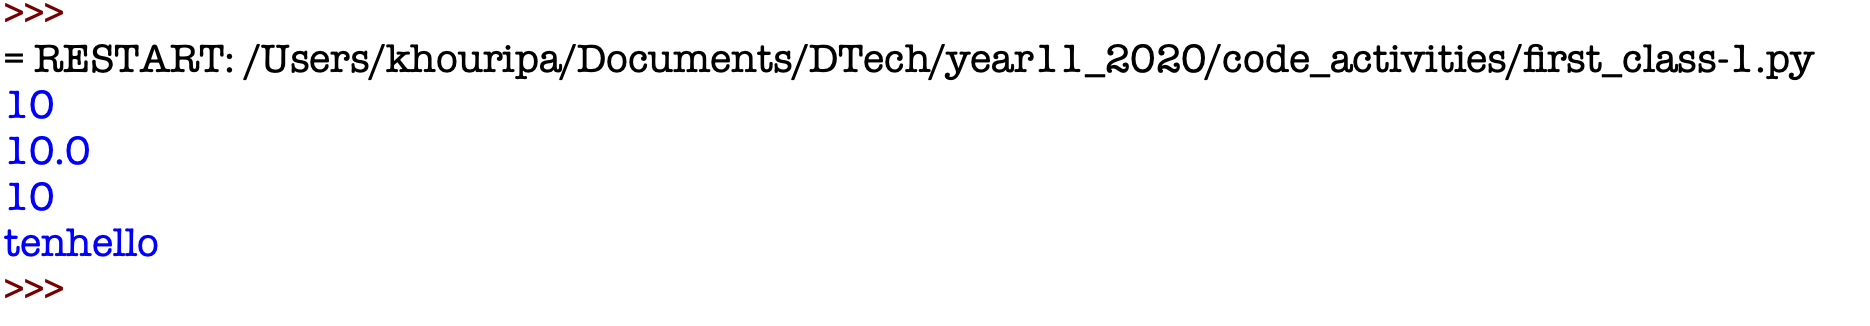
\includegraphics[width=18cm]{screen_shots/first_class-1.png}
	\caption*{Output}
\end{figure}
If the variables are numbers (integers or floats), we can use basic mathematical operations with them (+ , - , * , /).
\lstinputlisting[language=Python, caption=Python example
]{math_operations.py}

\begin{figure} [!h]
	\centering
	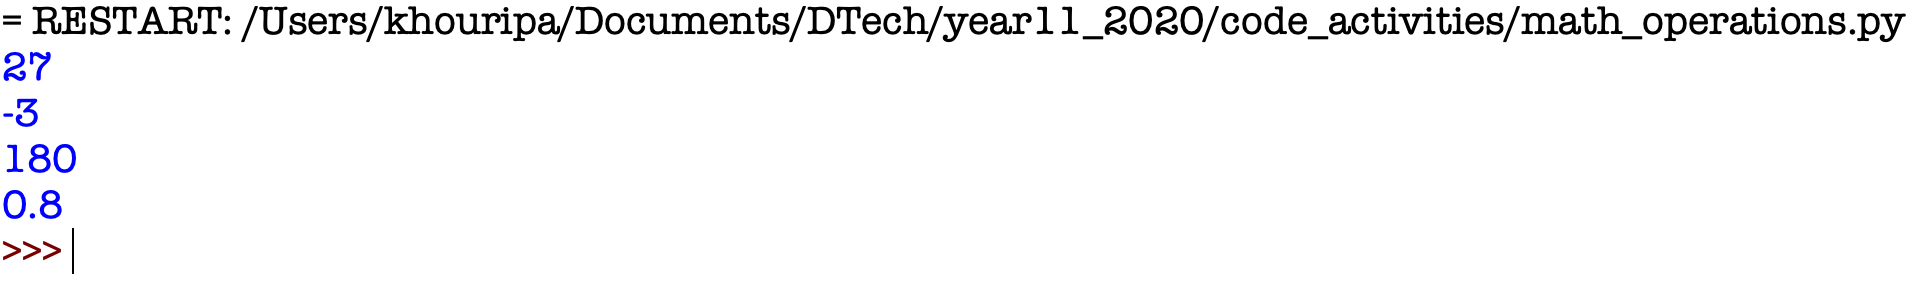
\includegraphics[width=18cm]{screen_shots/math_operations.png}
	\caption*{Output}
\end{figure}

\subsection{Variables  -- datatypes}
If we have a number such as 41834567, this could mean the value of 41 million .. or it just be a string of letters, for example, a phone number.\\
A program must know what type the variable is.\\
In the case above (and for lots of other situation), Python makes a “best guess”. In stricter languages you have define what type the variable is. \\
\lstinputlisting[language=Python, caption=Python example
]{first_class.py}

\begin{figure} [!h]
	\centering
	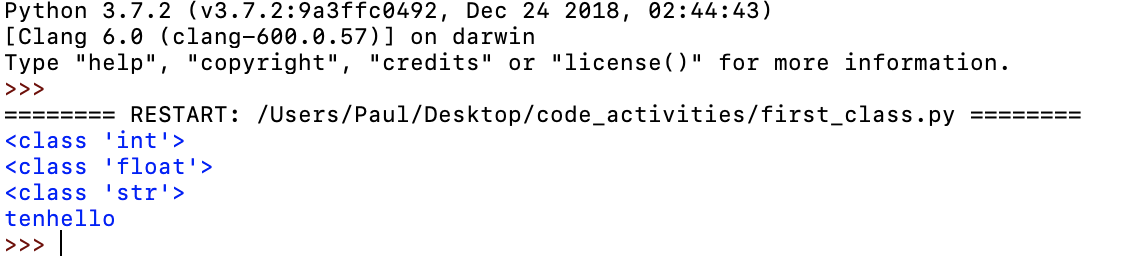
\includegraphics[width=18cm]{screen_shots/first_class.png}
	\caption*{Output}
\end{figure}

\newpage
\section{Inputs and Formatting}
The user input is held by a variable (which will be a string)\\
To get user input, use the input command and the message that will be printed in the console goes , as a string, in the brackets.\\
We can combine the information in the my\_string variable with another string , by using .format.
The variable referred to at the end is placed in the empty bracket.\\
Combining strings is called \textbf{concatenation}.

\lstinputlisting[language=Python, caption=Python example
]{input_format_output.py}

\begin{figure} [!h]
	\centering
	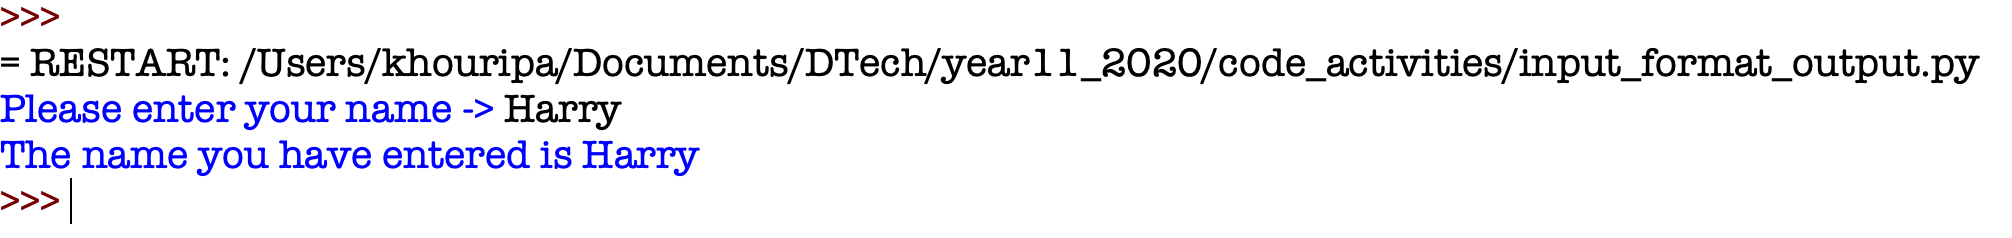
\includegraphics[width=18cm]{screen_shots/input_format_output.png}
	\caption*{Output}
\end{figure}

It is a good idea to be able to control output formatting very confidently:\\
See \url{https://www.w3schools.com/python/ref_string_format.asp}\\\\
Experiment with the following to get an idea about what the format method can do
\lstinputlisting[language=Python, caption=Python example]{formatting_examples.py}
\newpage
\section{Commenting}
When programs become more complex, it is helpful to write comments in the code.\\
Comments do not run in any way, they are just there for the programmer to read.\\
Comments are created by starting a line with a ``\#''.\\
Comments are \textbf{essential}
\lstinputlisting[language=Python, caption=Python example]{formatting_examples_comments.py}
\newpage
\section{Casting}
At times we need to change a data type and the most common situation is to turn a string into a number (float or integer) or to go the other way.\\
To do this we need to \textbf{cast} the variable to a new data type.
\lstinputlisting[language=Python, caption=Python example]{casting.py}



\begin{figure} [!h]
	\centering
	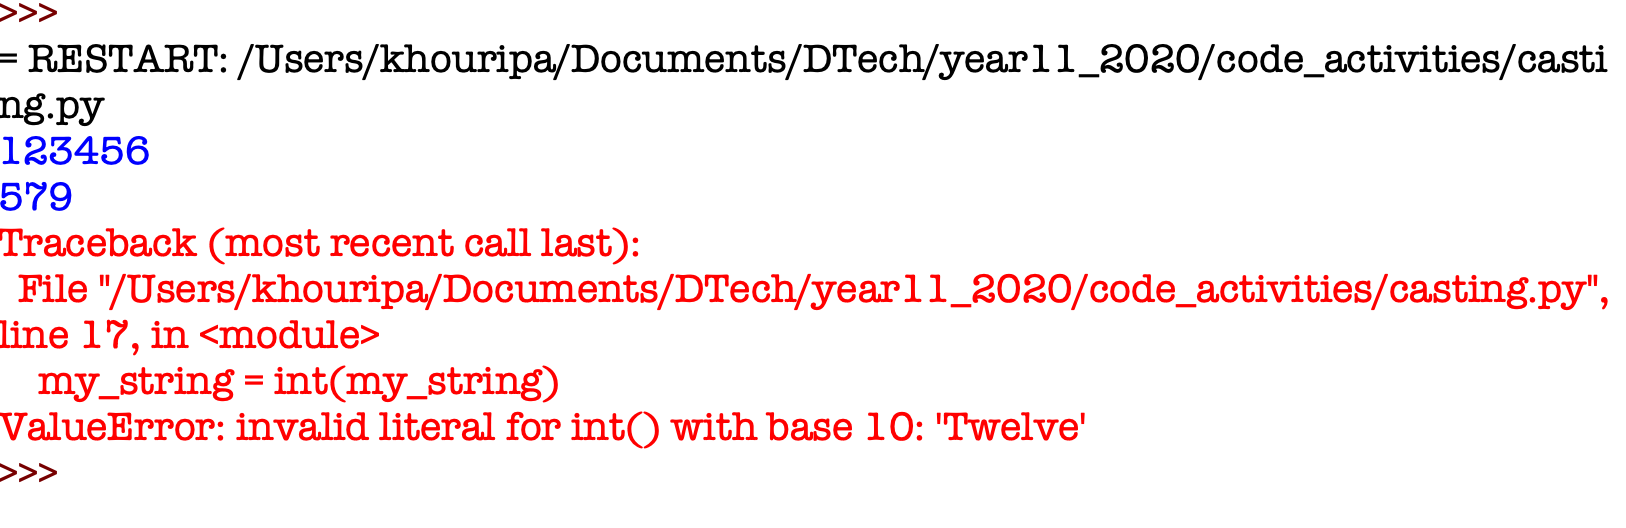
\includegraphics[width=18cm]{screen_shots/casting.png}
\end{figure}
\newpage
\section{Dinner Order - Basic Program - Design and Build}
You need to create a program that allows a waiter to enter in the number of main meals ( at \$12.50 each ) , the number of desserts ( at \$6.00 each ) and the number of drinks ( at \$3.55 ) ordered at a table.\\
The program then prints out a summary of the order, a total and then adds on GST (and gives the new total ).\\
(Note: the program should be easy to alter so the price values should be declared as constant variables)


\begin{figure} [!h]
	\centering
	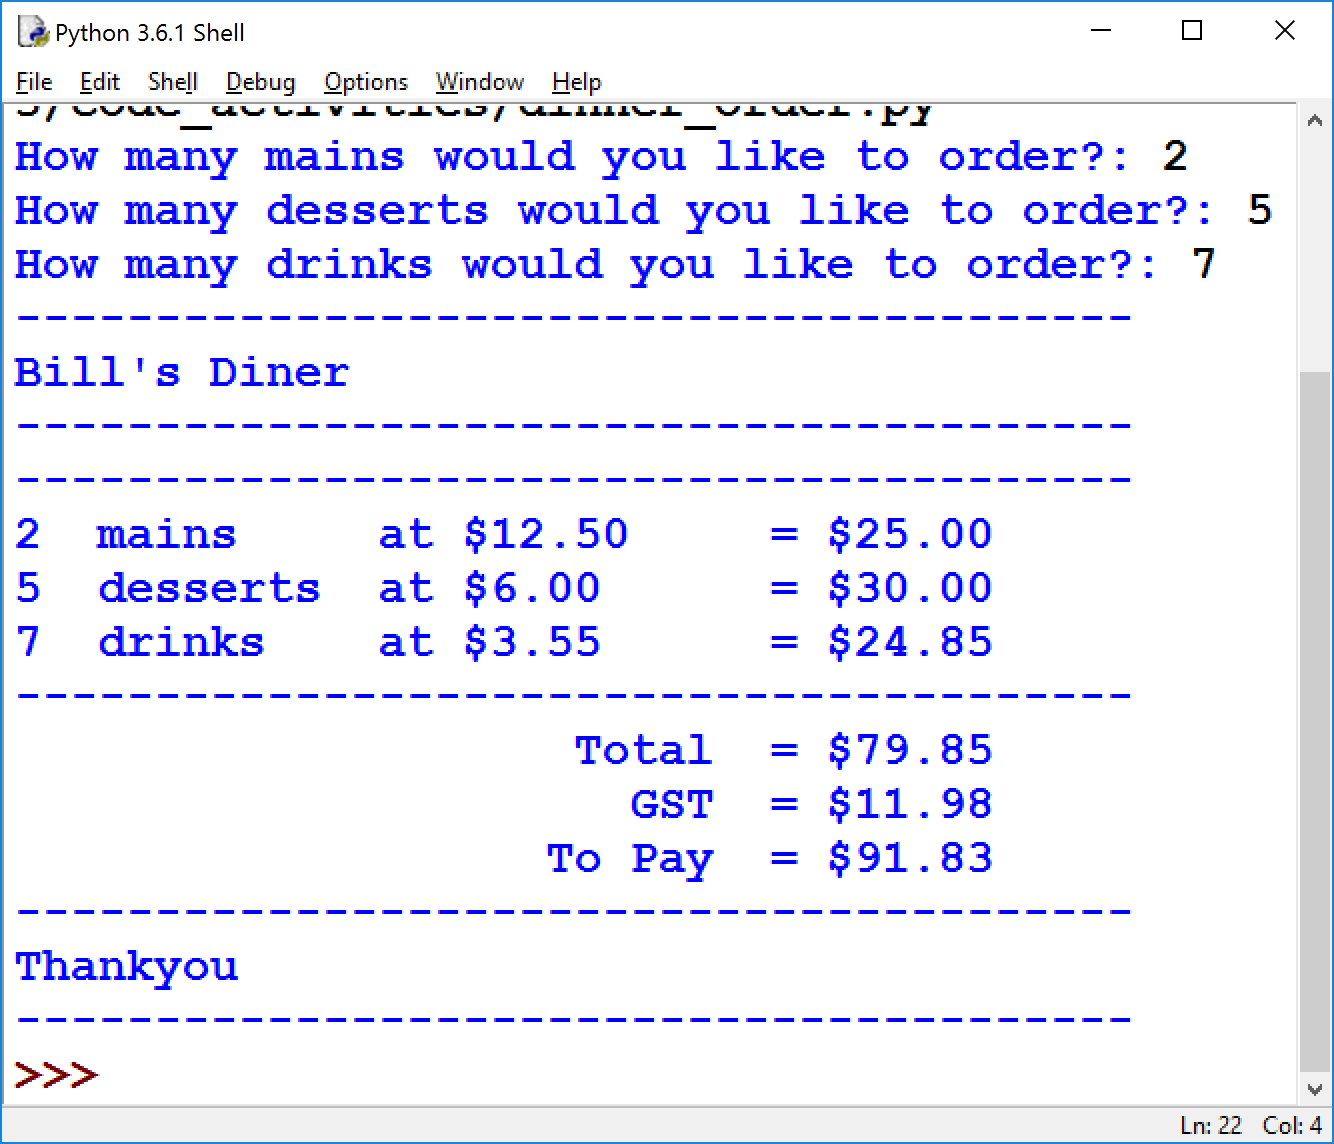
\includegraphics[width=10cm]{screen_shots/diner.png}
	\caption*{An example of Dinner Order program run}
\end{figure}


\subsubsection{Planning and Testing}
Much of the planning work for a program is done on paper (and will need to be photographed and placed in a document)\\
The testing is done on the computer and is documented.\\\\
A basic idea of the process is given below (but we will expand on this as things go)
\begin{itemize}
	\item \textbf{Breaking the problem down into components (or sub- problems)}:\\
	This means identifying the key things the program needs to do.

\item \textbf{Writing Pseudo code}\\
This means sketching out in writing or diagrams how the code is going to be put together. (the writing should communicate how the code is going to work, but does not need to be the exact language) 
\item \textbf{Building and Trialling}\\
Build the program in stages and trial each stage as you go.
\item \textbf{Assembled Outcome Testing}\\
Once you have got the program made, there needs to be some formal testing of it. \\
Errors need to be identified 
\item \textbf{Usability Testing}\\
Ideally the program should be tested on some other user other than yourself
\item \textbf{General Evaluation:}\\
A basic reflection
\end{itemize}

\newpage
\textbf{Examples of Component Planning}\\
\begin{figure} [!h]
	\centering
	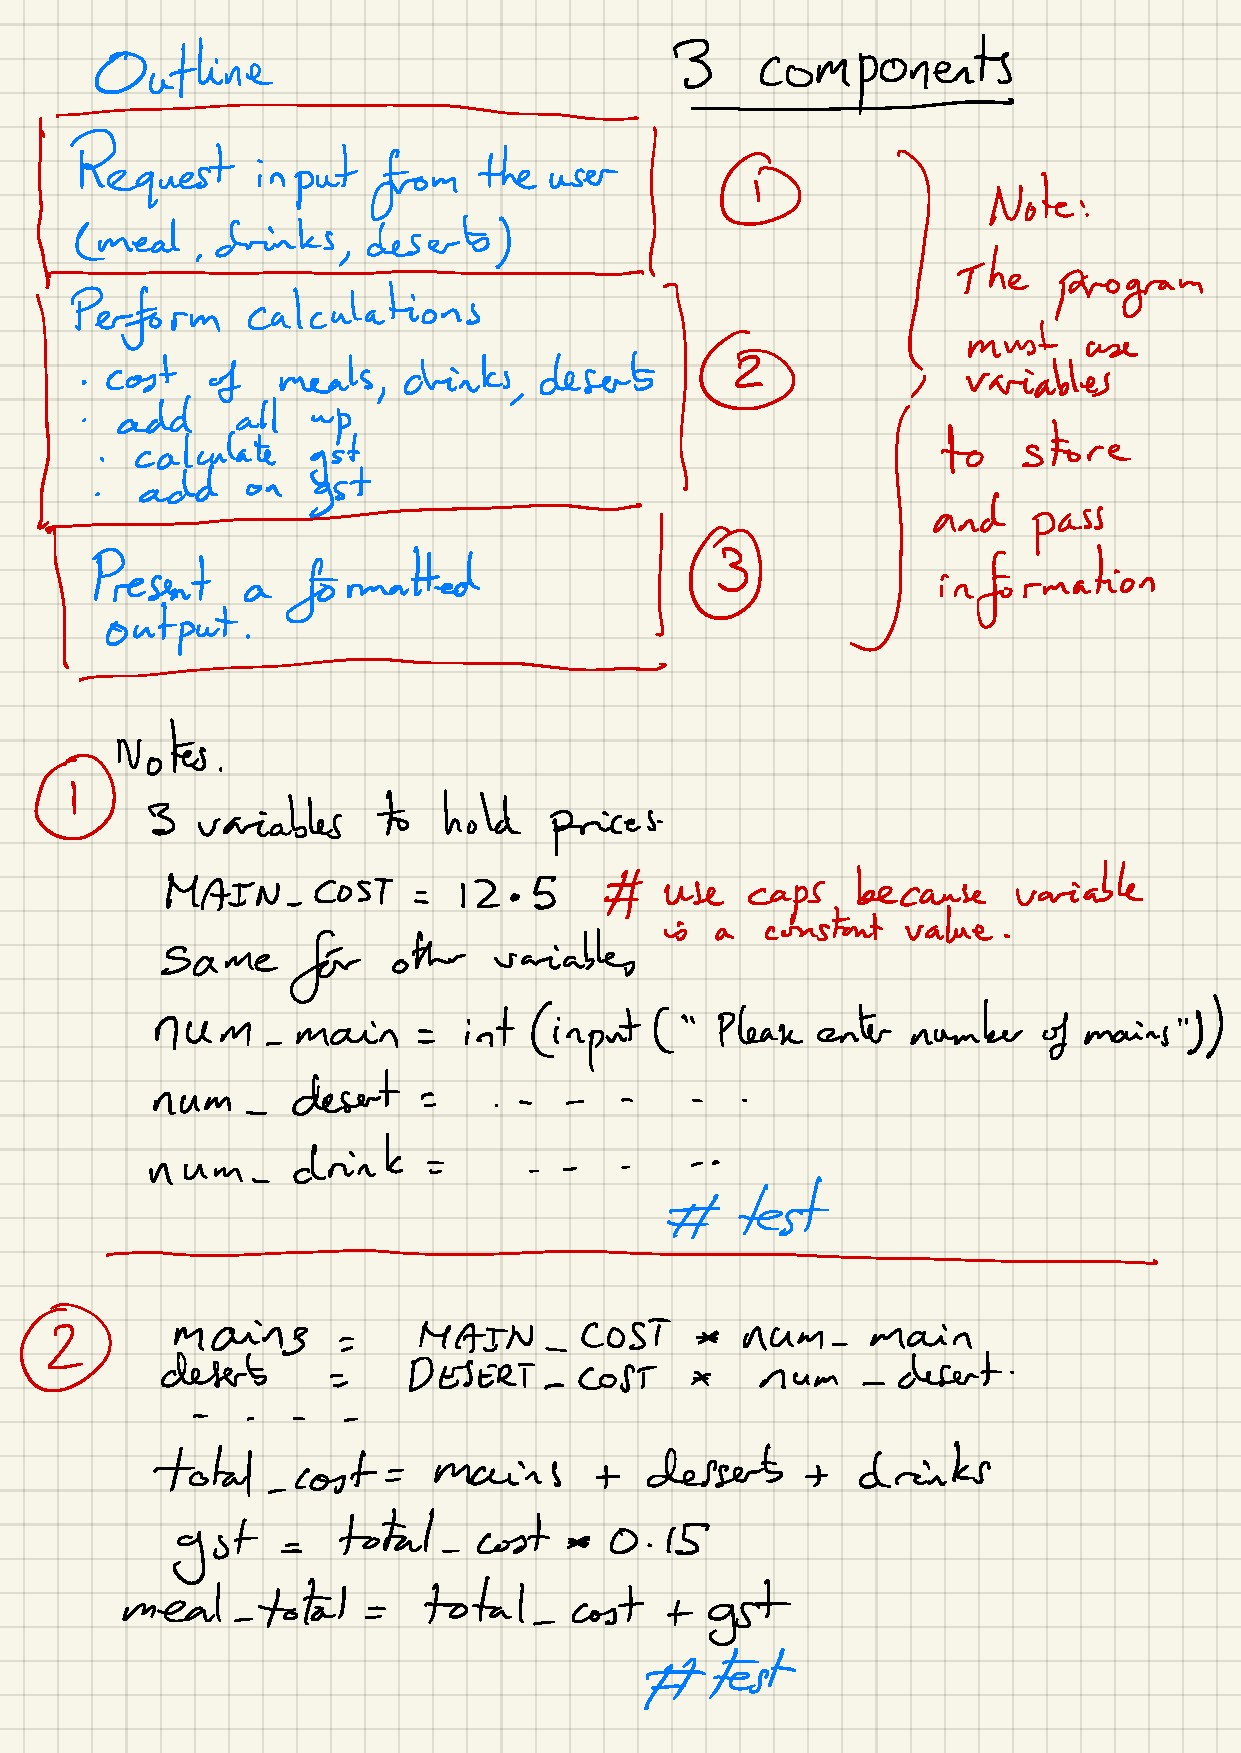
\includegraphics[width=12cm]{iterative_processes/simple_planning_1.pdf}
\end{figure}
\begin{figure} [!h]
	\centering
	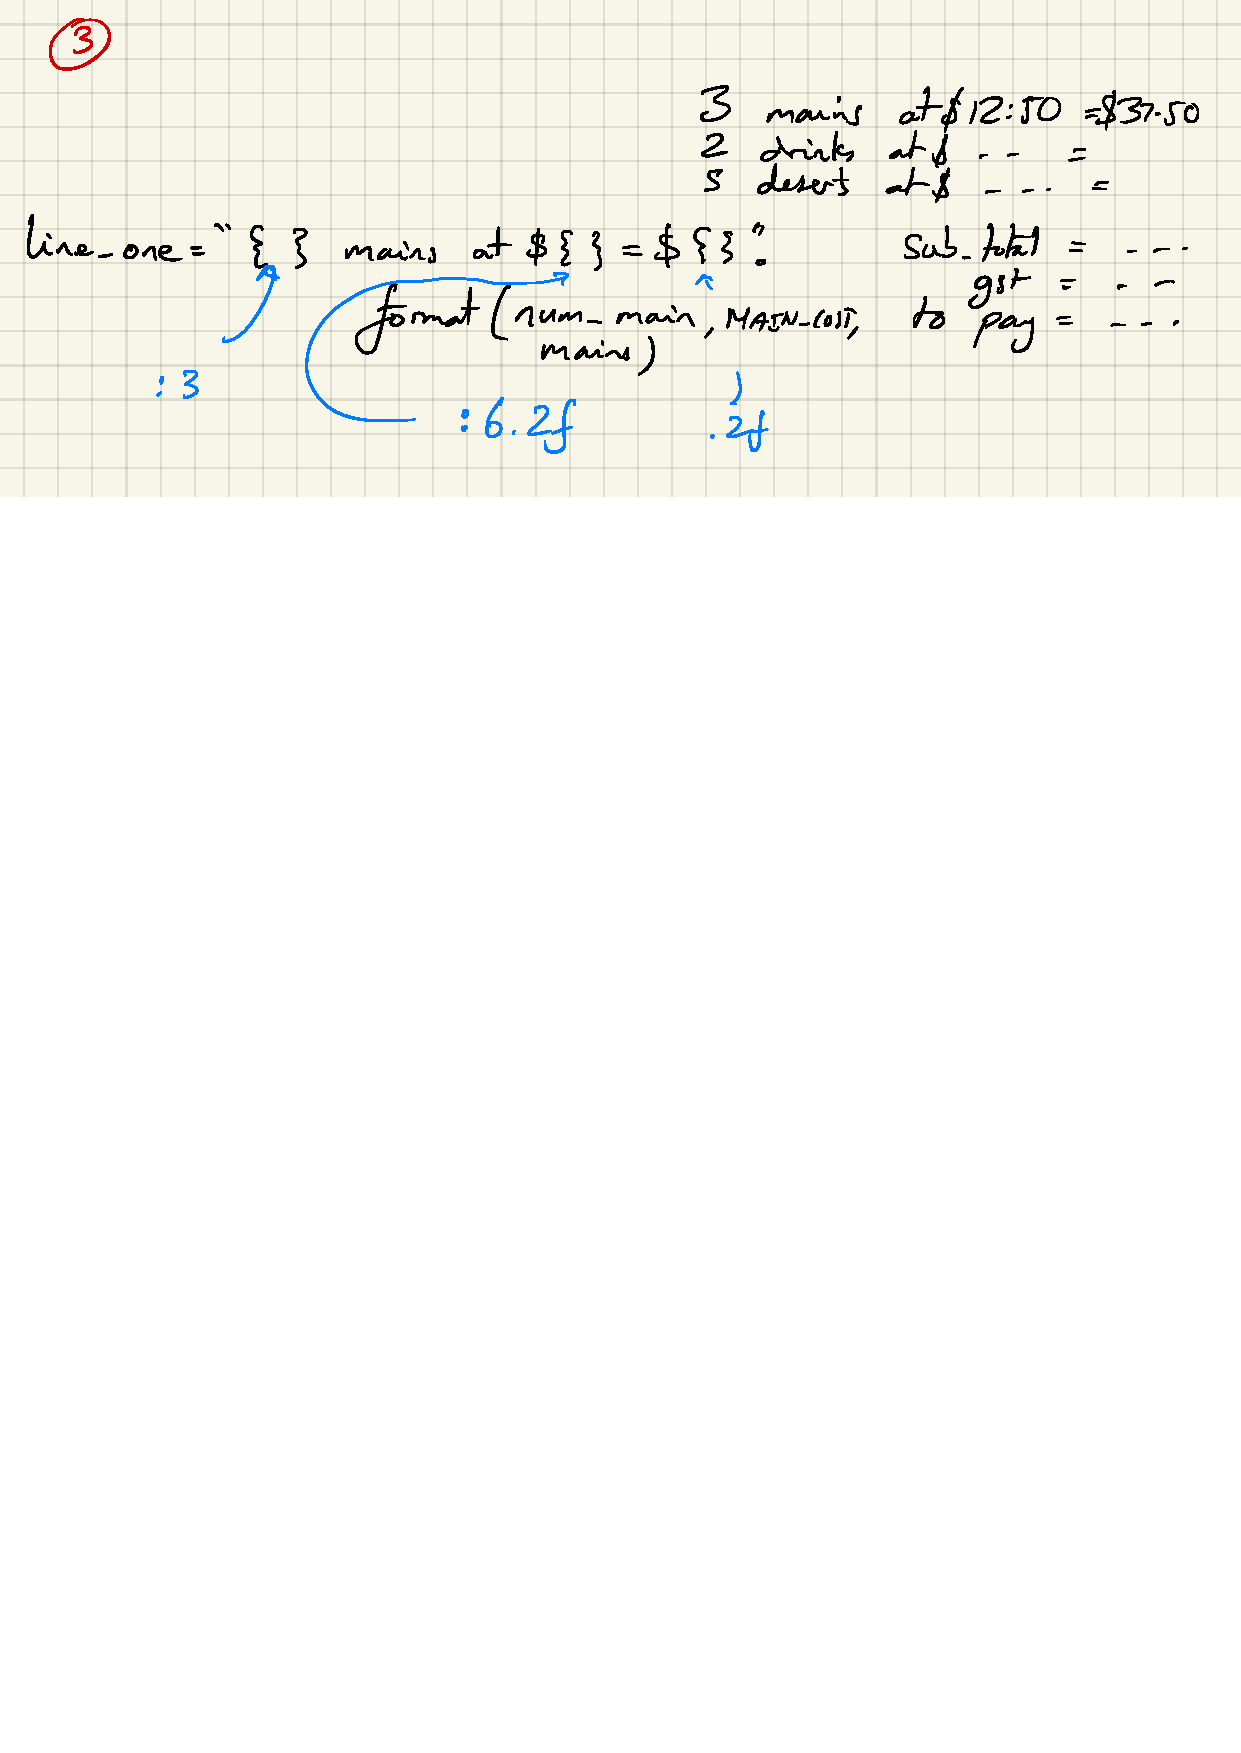
\includegraphics[width=12cm]{iterative_processes/simple_planning_2.pdf}
\end{figure}
\newpage
\textbf{Basic Idea of Testing}
When testing we consider
\begin{itemize}
	\item Expected inputs (these are inputs we would normally expect the user to input).\\
	Does the program give the right outputs with the given expected inputs.
	\item Boundary inputs (are there maximum or minimum value that the user can enter)\\
	What happens at these \underline{boundaries} (and if we go over them)
	\item Unexpected Inputs  (these are character entries that we are not expecting)\\
	These could be just pressing enter or having spaces , using letters instead of numbers or characters like * , \&, etc.\\
	These could occur if the user makes a mistake or misunderstands what is expected.
\end{itemize}
Testing should have some kind of plan and documentation of the results.\\

\begin{figure} [!h]
	\centering
	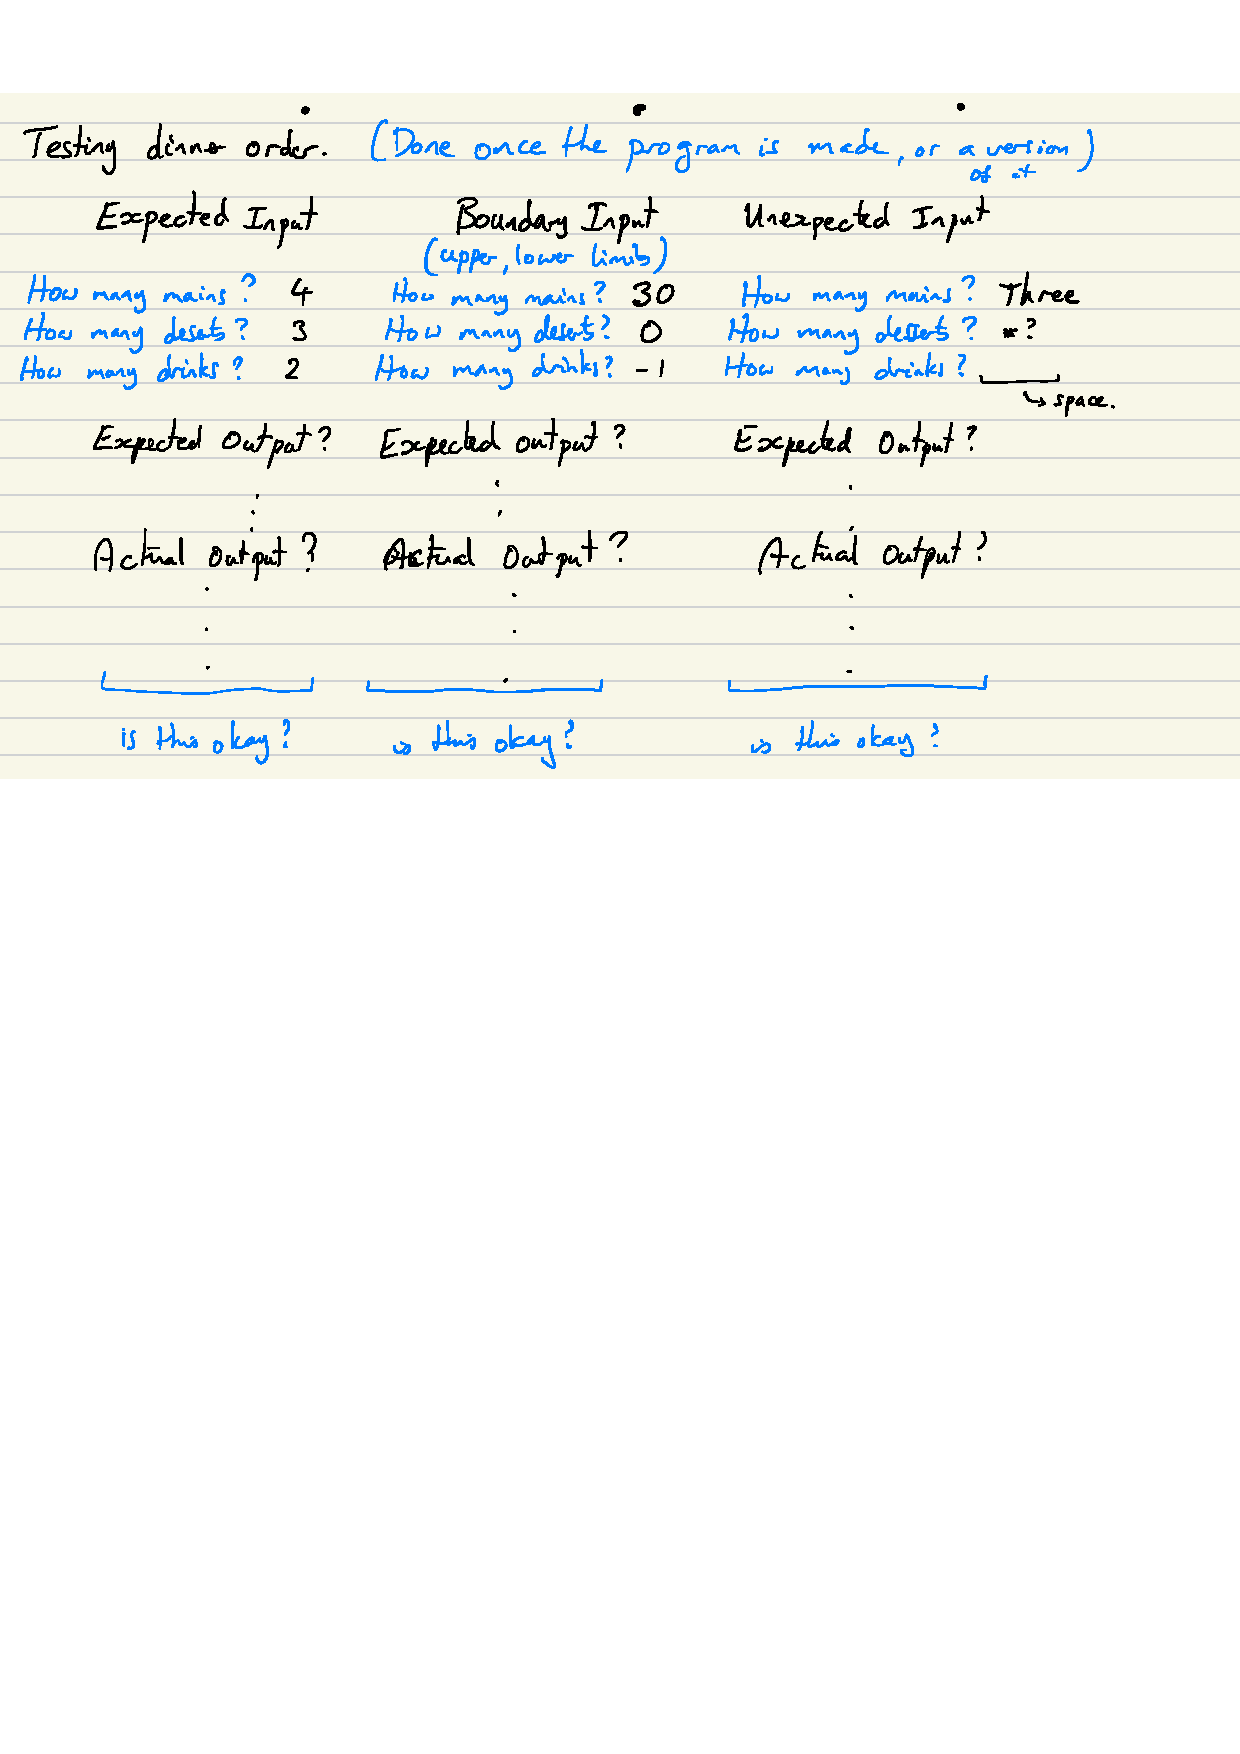
\includegraphics[width=16cm]{iterative_processes/Testing.pdf}
\end{figure}

\begin{figure} [!h]
	\centering
	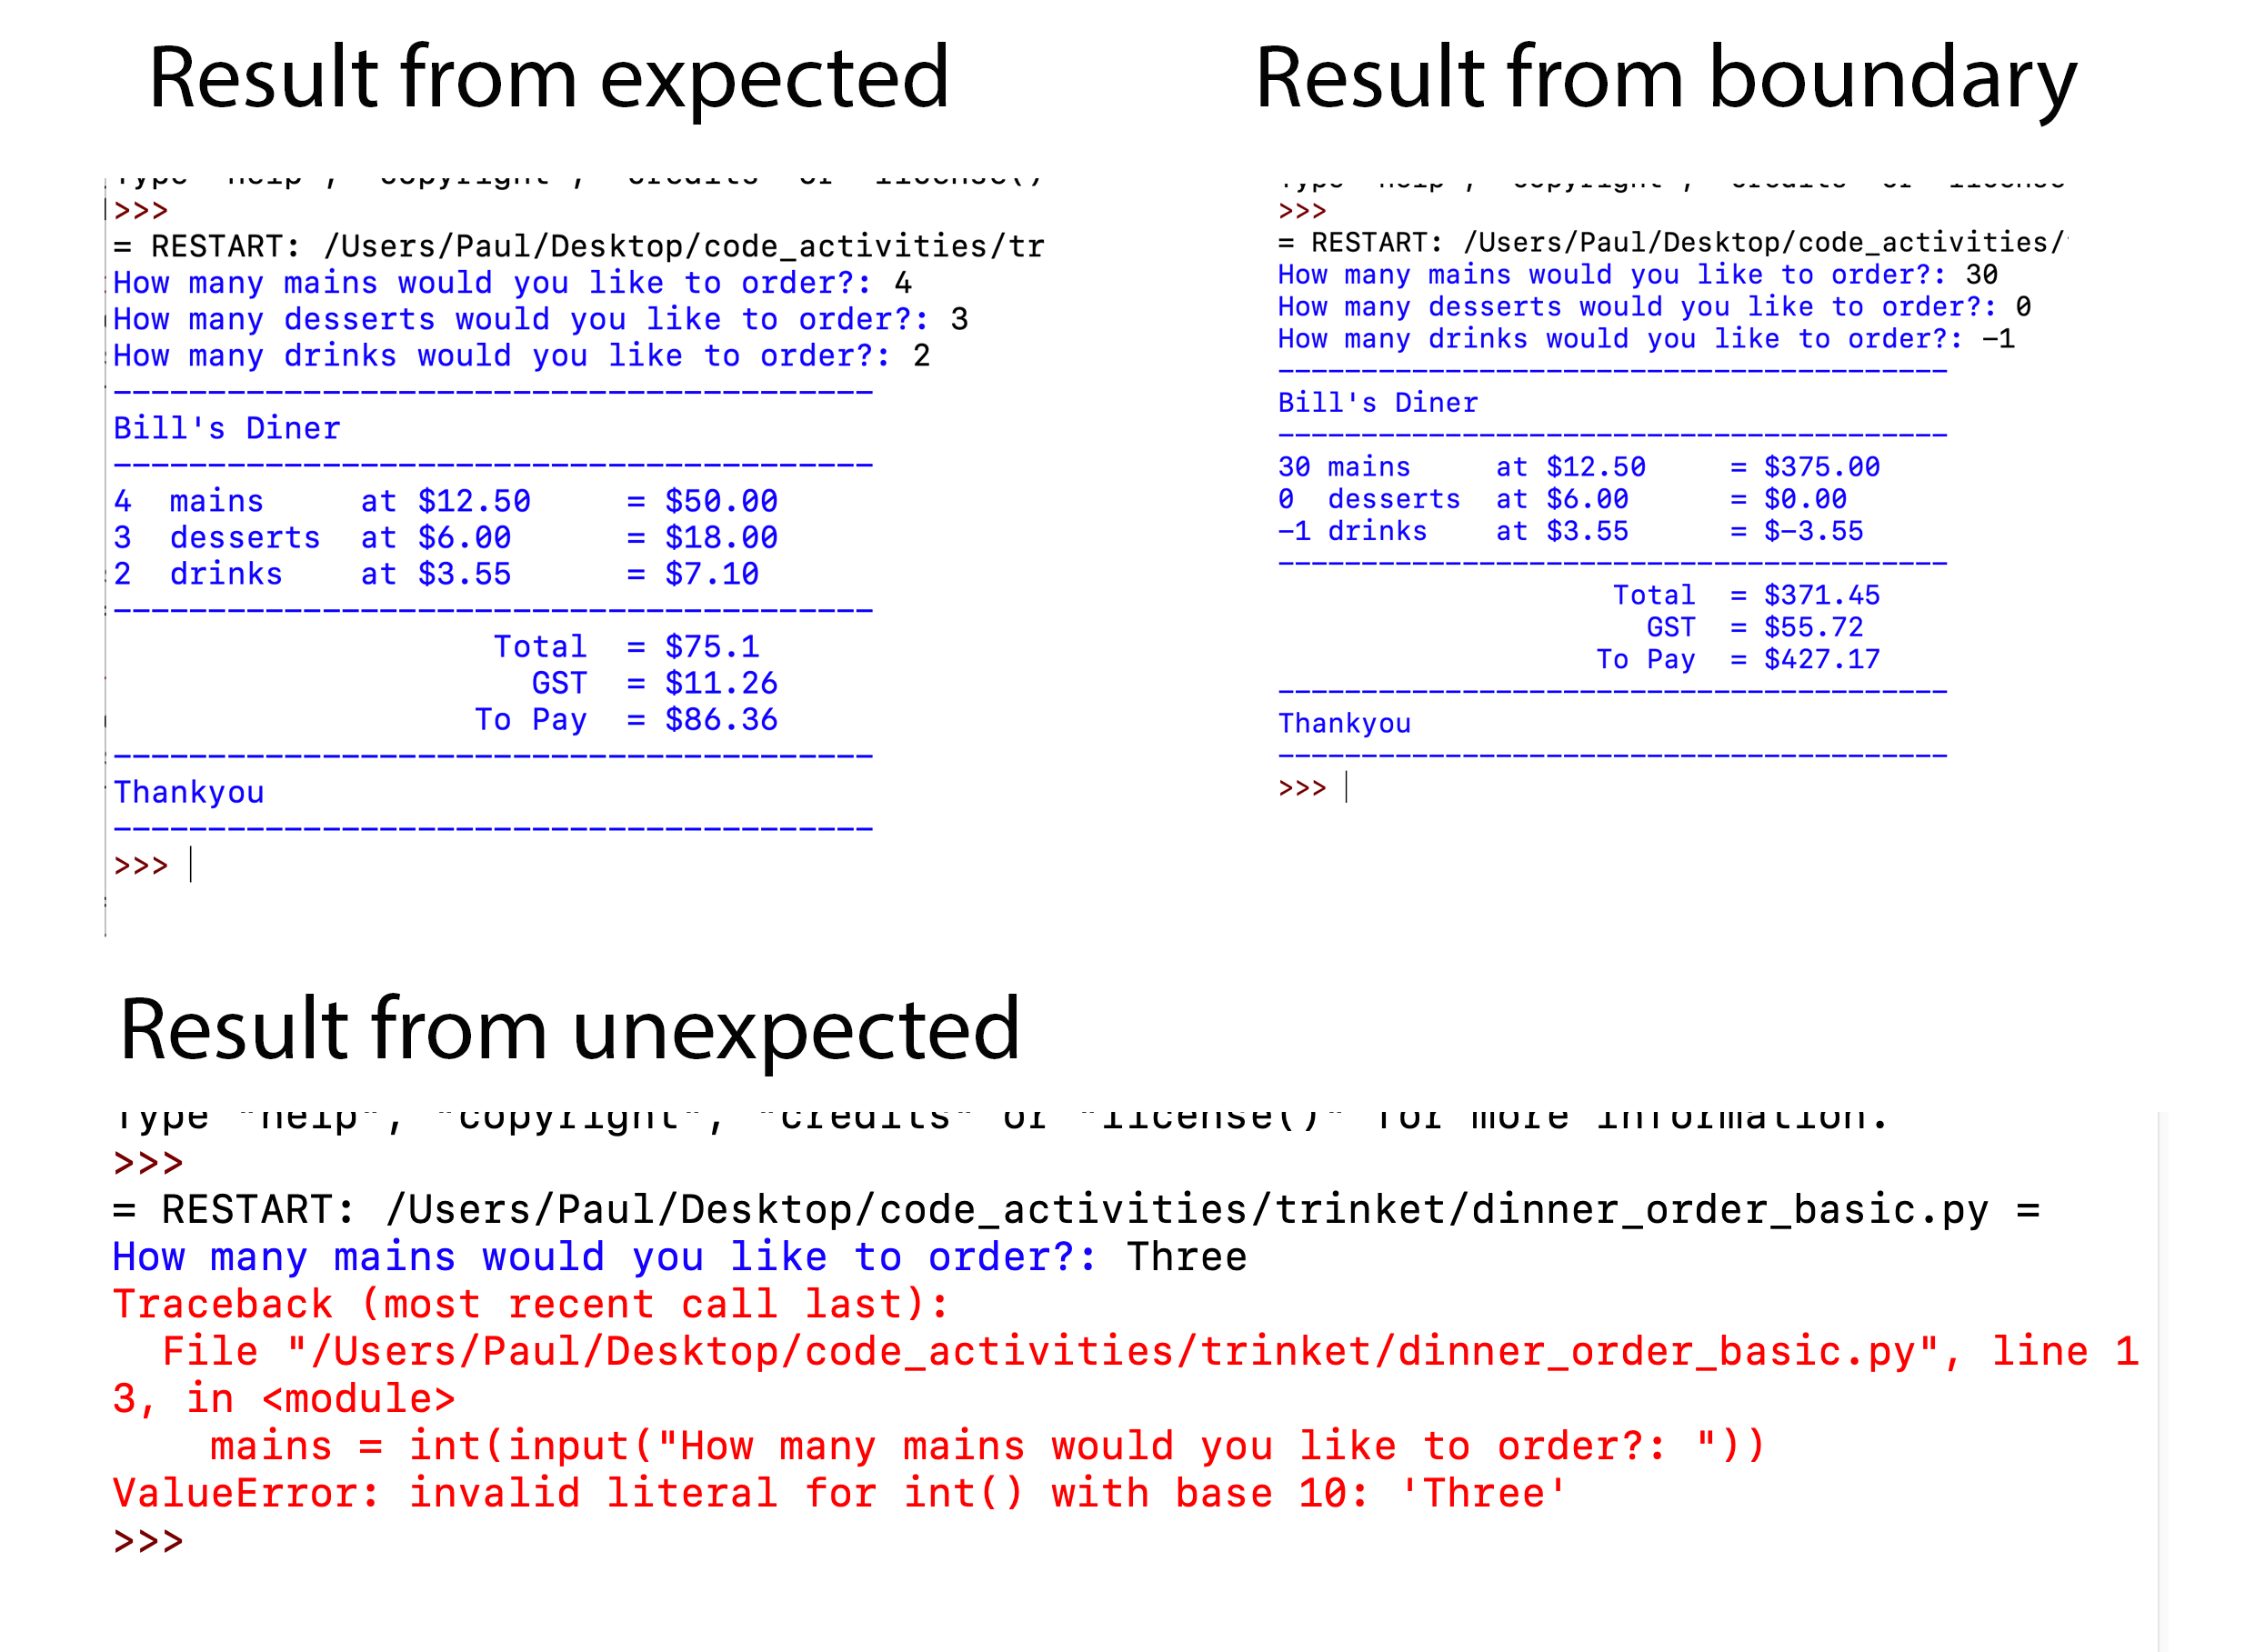
\includegraphics[width=16cm]{iterative_processes/Testing.png}
\end{figure}
\newpage
\textbf{Evaluation}
\begin{itemize}
	\item What works 
\begin{itemize}
	\item Works properly on expected inputs
	\item Presentation of reciept clearly laid out on console.
\end{itemize}
	\item What could be improved
\begin{itemize}
	\item Should have an upper limit on how many meals can be entered
	\item Should not allow entries below zero
	\item Unexpected inputs cause a program crash
	\item At the moment the program only runs once (so need a way to enter a new order)
\end{itemize}
\end{itemize}
\newpage







\newpage
\subsection{Strawberry picking}

A strawberry farm lets families come and pick strawberries. \\
They can fill boxes, buckets or punnets (any combination).\\
\begin{itemize}
	\item They charge a rate of 5 \$/kg. 
	\item Full of strawberries, a punnet weighs 250 g, a box weighs 1.5 kg and a bucket weighs 7 kg.
\end{itemize}
Design a program that calculates the amount to be charged given a certain number of boxes, punnets and buckets have been picked.

\begin{figure} [!h]
	\centering
	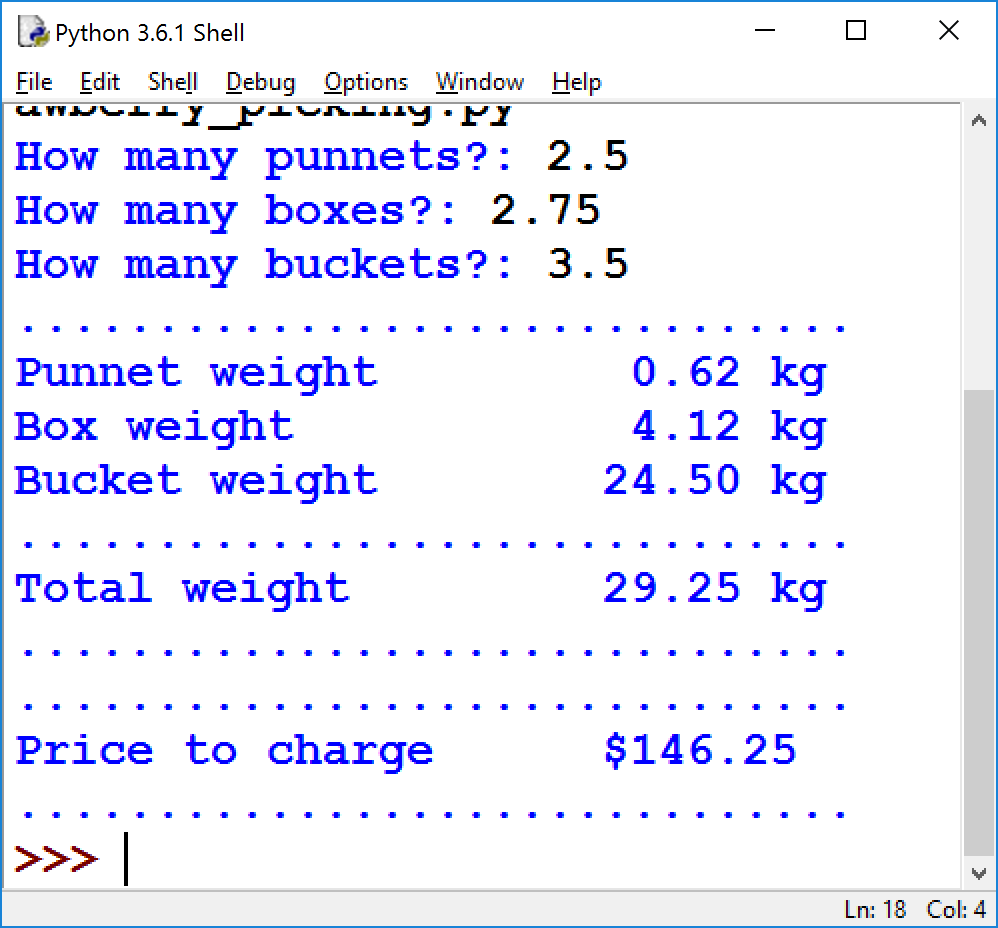
\includegraphics[width=10cm]{screen_shots/strawberries.png}
	\caption*{An example of Strawberries program run}
\end{figure}
\newpage


\newpage
\section{Conditions}
The solutions to many programming problems require an action to occur only if a particular condition is true.\\ 
A condition can only result in true or false. \\
(These values are called Booleans. True and False are reserved words in the Python language. True and False are values / objects of type bool)\\
A condition often involves an expression which compares one value with another.\\
Comparisons between numerical values are made using the same comparison operators that are used in mathematics:\\
\begin{align*}
> & \text{~~~~~~greater than}\\
>= & \text{~~~~~~greater than or equal to}\\
< & \text{~~~~~~less than}\\
<= & \text{~~~~~~less than or equal to}
\end{align*}
 and the equality / inequality operators:
 \begin{align*}
 ==  & \text{~~~~~~equal to ( the proper equals operator)}\\
 != & \text{~~~~~~not equal to}
 \end{align*}
\textbf{Boundary cases}\\
Human languages are imprecise. \\
Does "every child over 5" mean "aged 5 and over" or "aged 6 and over"? The difference between $>=$ and $>$ is very important. \\
If you mean "every child aged 5 and over" you can express this as age $> 4$ or age $>= 5$.\\
Any lack of clarity needs to be removed at the design phase. Always clarify before
coding. The boundary cases are where errors in programming often occur.\\
 Boundary cases are the values at and just outside the specified limits.\\
 In the case "aged 5 and over" the specified limit is 5 and the age values of 4 and 5 are the boundary cases.
 \newpage
 \begin{figure} [!h]
 	\centering
 	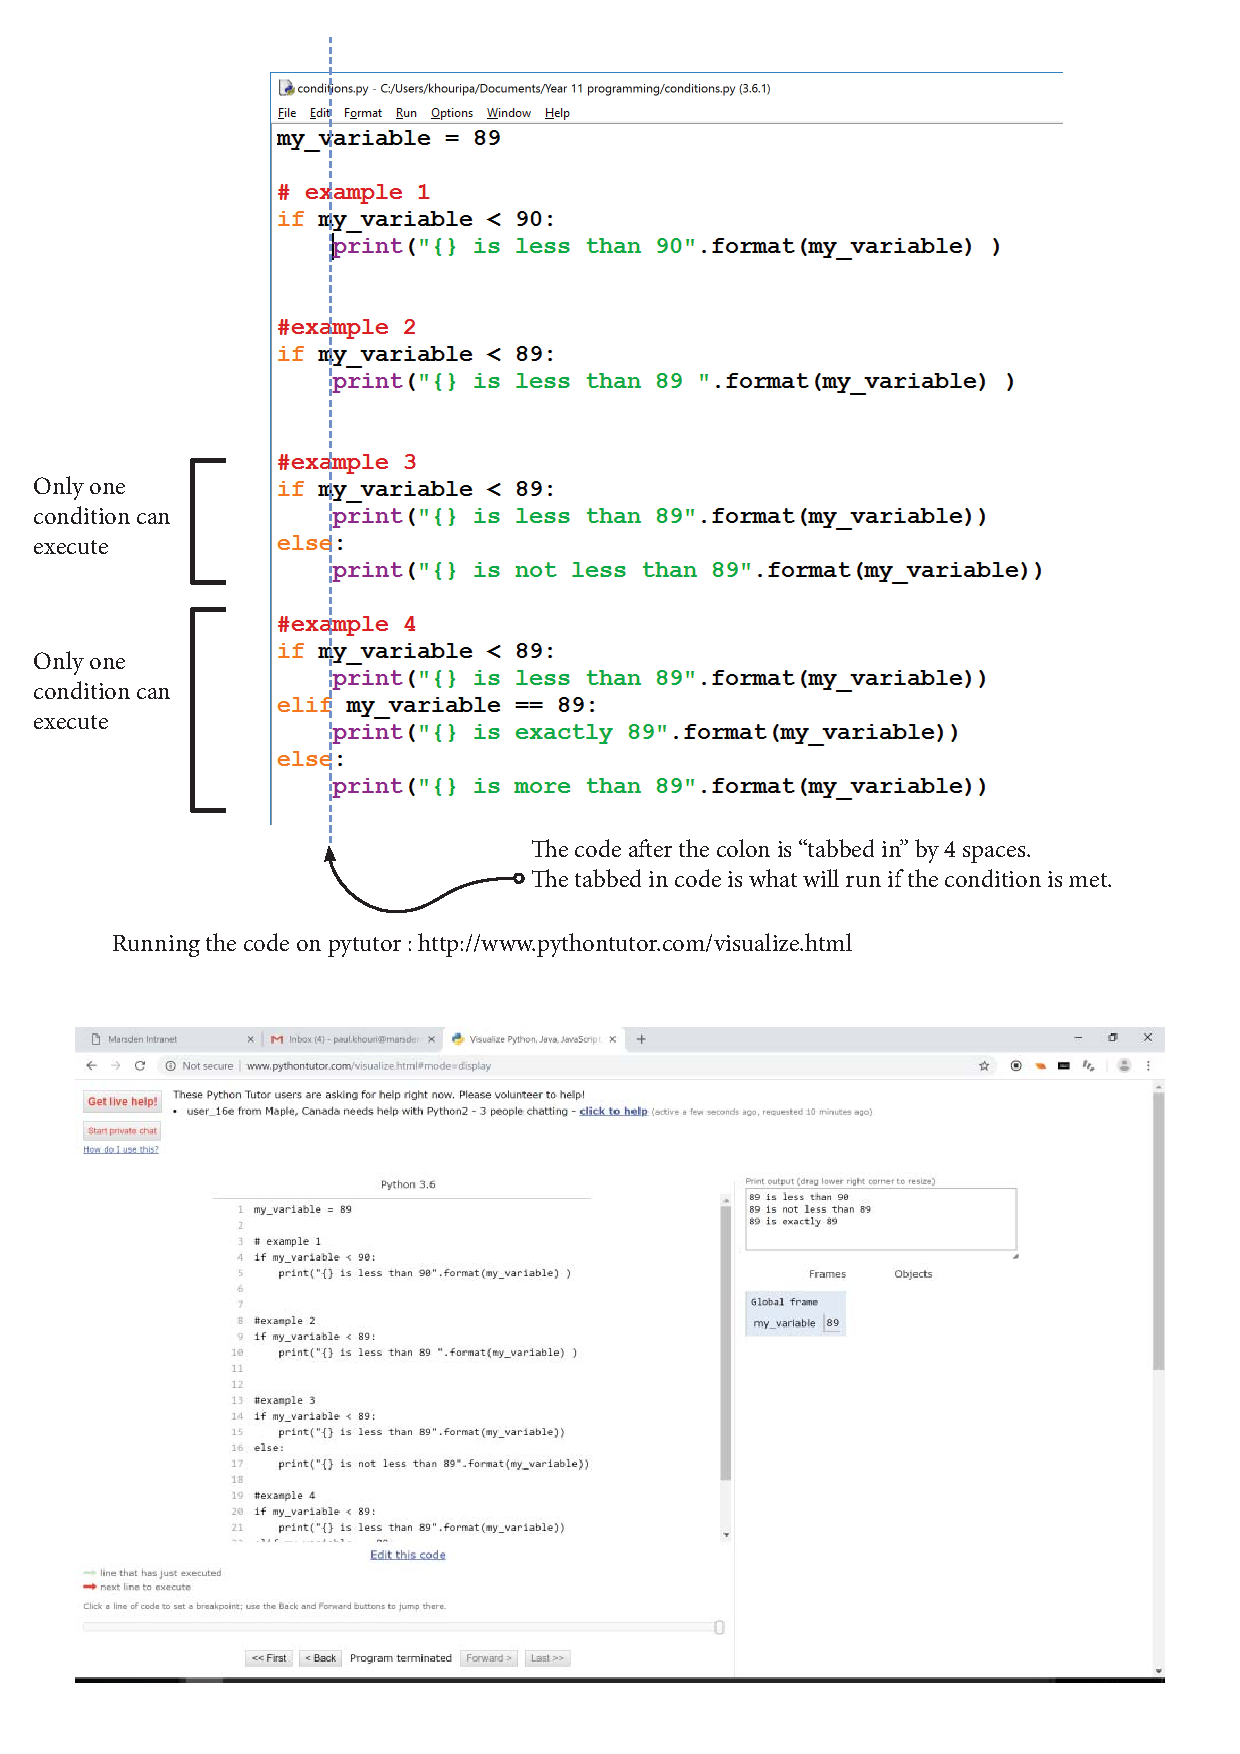
\includegraphics[width=17cm]{screen_shots/conditions.pdf}
 \end{figure}
\newpage
\lstinputlisting[language=Python, caption=Conditions Examples]{conditionals/examples.py}
\subsection{Activities (conditions) }
\begin{enumerate}[label=\normalsize \alph*)~~~ , topsep=8pt,itemsep=25pt,partopsep=4pt, parsep=4pt, leftmargin = 0.5cm]
	\item Write a program that asks `What will the max temperature today?'\\
	If the temperature is below 10$\degree$ ,  print `Cold today' , if between 10$\degree$ and 20$\degree$, prints 'Regular Wellington day today' and if over 20$\degree$ prints `Hot today'.\\
	\textbf{Test table:}\\
	\begin{tabular}{| p{5cm} | p{5cm} | p{5cm} |}\hline
	Test input& Expected output & Actual output\\\hline
	&  &  \\\hline
		&  &  \\\hline
			&  &  \\\hline
	\end{tabular}
\item Write a program that has a variable  `allowance' set to 5, and asks a 'Yes/No' input , `Have your helped clean the kitchen?',\\
If the user has, then add \$2.00 dollars to the allowance and if not add \$1.00 to the allowance.\\
Print out appropriate feedback.\\
	\textbf{Test table:}\\
	\begin{tabular}{| p{5cm} | p{5cm} | p{5cm} |}\hline
	Test input& Expected output & Actual output\\\hline
	&  &  \\\hline
	&  &  \\\hline
\end{tabular}\\

Extend this to include `Have your helped to put the garbage out?'.\\
 If the user has done both add \$4.00 to the allowance, if they have done one of the two, add \$2.00 if none add \$1.00.\\
 	\textbf{Test table:}\\
	\begin{tabular}{| p{5cm} | p{5cm} | p{5cm} |}\hline
	Test input& Expected output & Actual output\\\hline
	-\newline -&  &  \\\hline
	-\newline -&  &  \\\hline
		-\newline -&  &  \\\hline
			-\newline -&  &  \\\hline
\end{tabular}
\newpage
\item Using variables a, b, c in a program, each one is associated with an input asking to enter a number.\\
Print out the minimum number. (Do not use Python's `min' method , use conditional statements).\\
	\textbf{Test table:}\\
	\begin{tabular}{| p{5cm} | p{5cm} | p{5cm} |}\hline
	Test input& Expected output & Actual output\\\hline
	-\newline - \newline -&  &  \\\hline
	-\newline - \newline -&  &  \\\hline
		-\newline - \newline -&  &  \\\hline
\end{tabular}

\item 	To go to university a person needs to be:
\begin{itemize}
	\item over the age of 20
	\item \textbf{or} be 16 or older and have level 3 NCEA 
	\item \textbf{and} (for both conditions) the person need to be competent with English.
\end{itemize} 
Create a program that given the following variables:\\
age= 25\\
ncea = False\\
english = True\\
Will give a correct response about whether a person can go to university or not.\\
Do not worry about inputs , just test by changing the variables.\\
Test with other values.
	\textbf{Test table:}\\
		\begin{tabular}{| p{5cm} | p{5cm} | p{5cm} |}\hline
		Test input& Expected output & Actual output\\\hline
		-\newline - \newline -&  &  \\\hline
		-\newline - \newline -&  &  \\\hline
		-\newline - \newline -&  &  \\\hline
	\end{tabular}
\end{enumerate}

\newpage
\subsubsection{Solutions}
\lstinputlisting[language=Python, caption=Worksheet Solutions]{conditionals/worksheet_solutions.py}
\newpage

\section{Random numbers}
Random numbers are particularly useful for games and quizzes as they mean that the program will not always do things in the same order.\\
To get random numbers we need to import a \textbf{library} that handle random numbers.\\
Python has a large number of libraries that extend the functionality of the programming language.

\lstinputlisting[language=Python, caption=Python example]{randomness.py}
\newpage
\section{Program using conditions and random numbers}
\subsection{Higher Lower}
This program is very simple (because we don't have loops yet ), but makes a useful base for future development.
\begin{itemize}
	\item Create a program that :\\
Generates a random number between two integers.
\begin{itemize}
	\item It asks the user to guess the number
	\item It then gives feed back about whether their guess is too small or too large or correct.
\end{itemize}
\item{Planning and Testing}
\begin{itemize}
	\item Write a psuedo code outline
	\item When the program is made, create and complete a test table ( introduce a small modification to the program to help you test it ) .
\end{itemize}

\begin{figure} [!h]
	\centering
	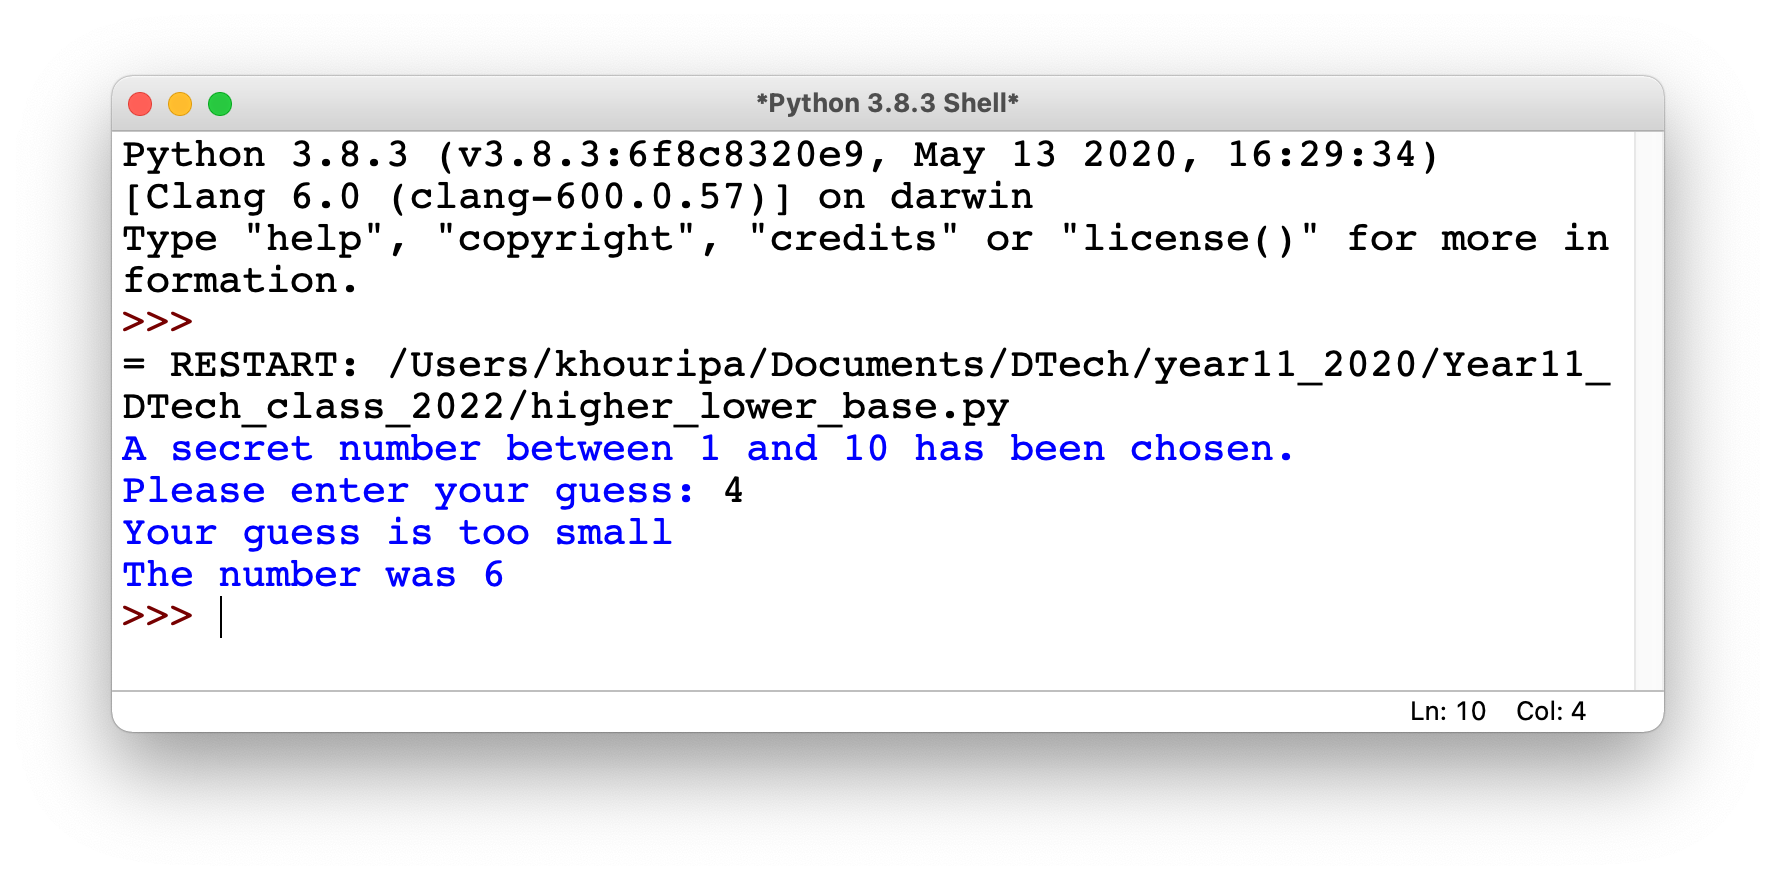
\includegraphics[width=13cm]{screen_shots/higher_lower_base.png}
	\caption*{An example of higher lower  program run}
\end{figure}

\end{itemize}
\newpage

\begin{figure} [!h]
	\centering
	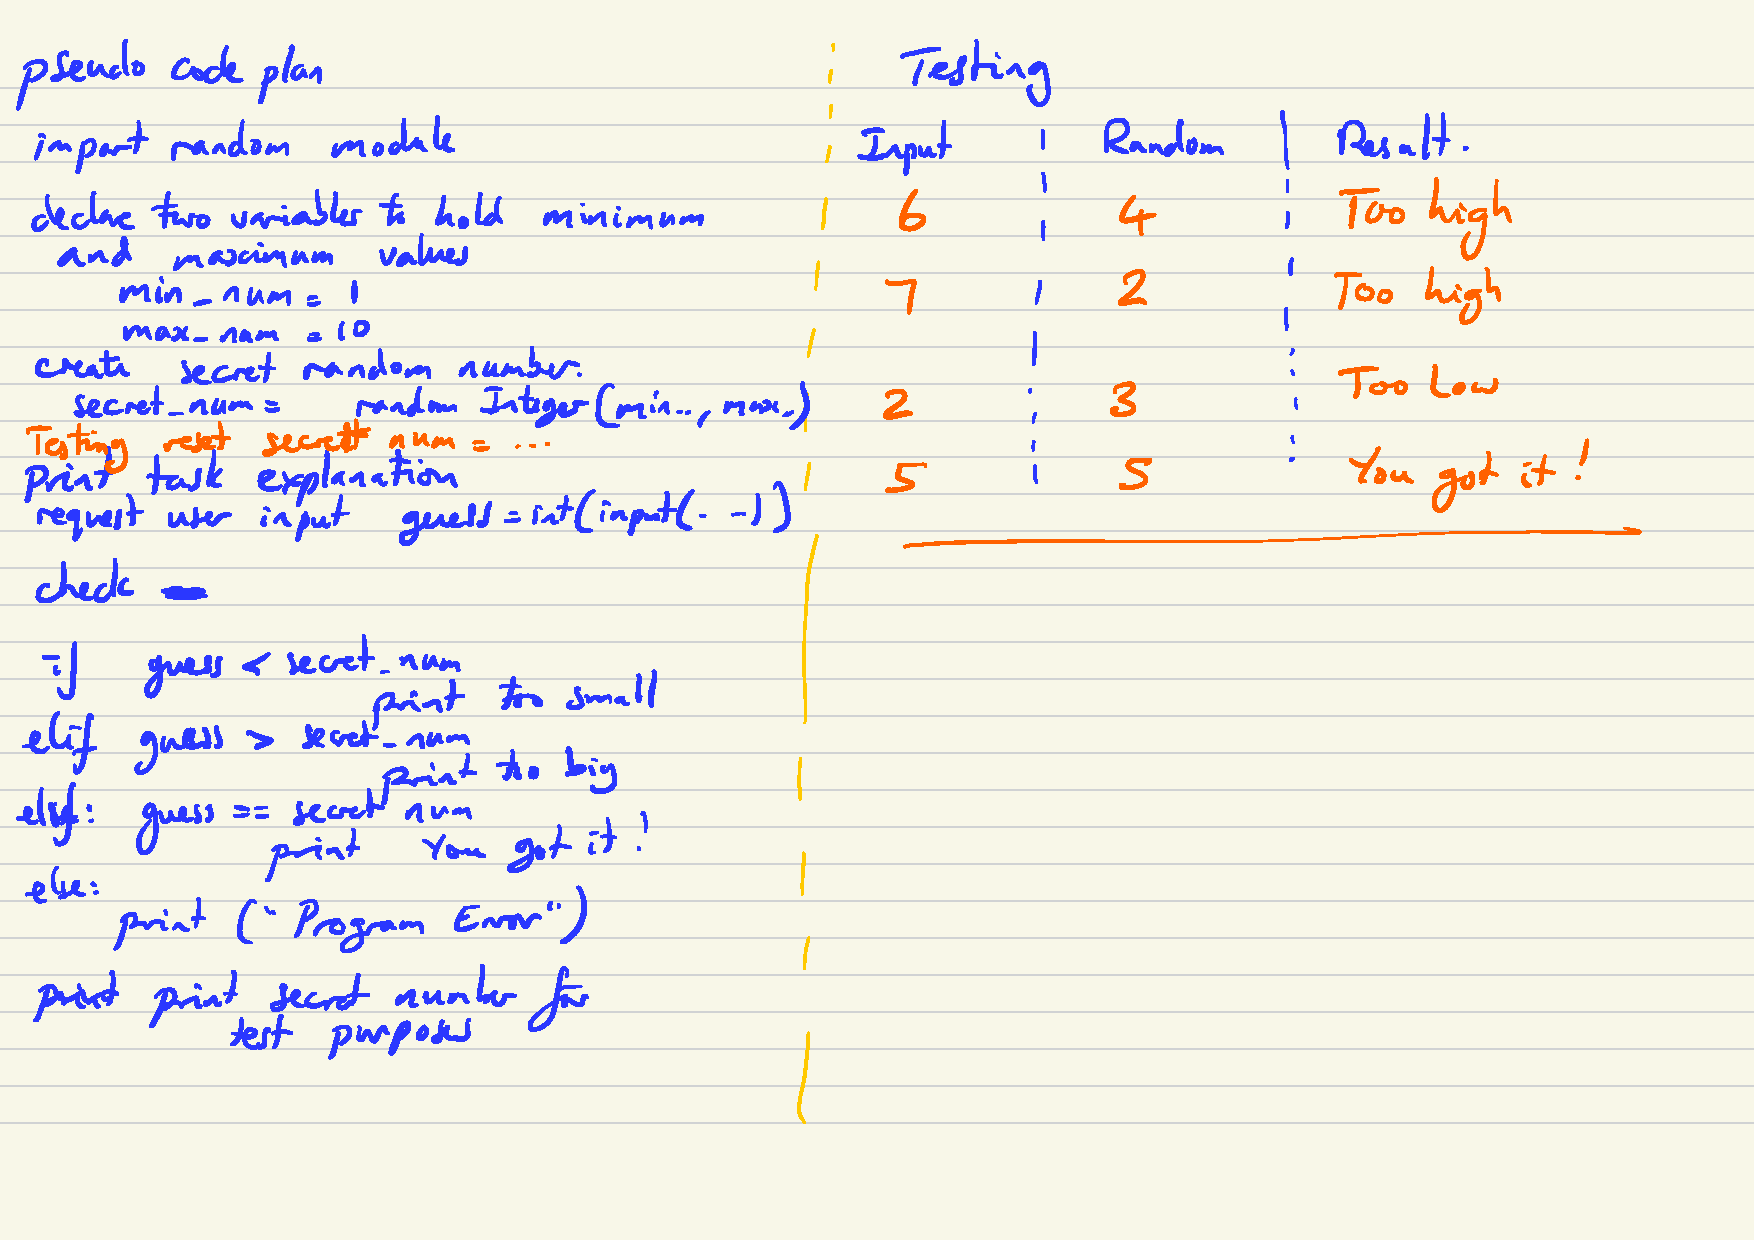
\includegraphics[width=17cm]{iterative_processes/Higher_lower_simple_plan.pdf}
	\caption*{Psuedo code and test grid}
\end{figure}
\lstinputlisting[language=Python, caption=Python example]{HigherLower/higher_lower_base.py}

\newpage
\section{Loops}
Often we want the the program to repeat some kind of operation or to repeatedly to run a section of code.\\
To do this we use loops.\\
The are \textbf{for} loops and \textbf{while} loops and we will focus on the while loop.\\

This while loop uses a counter to know how many times to run.
\lstinputlisting[language=Python, caption=Python example]{loop_counter.py}
 \begin{figure} [!h]
	\centering
	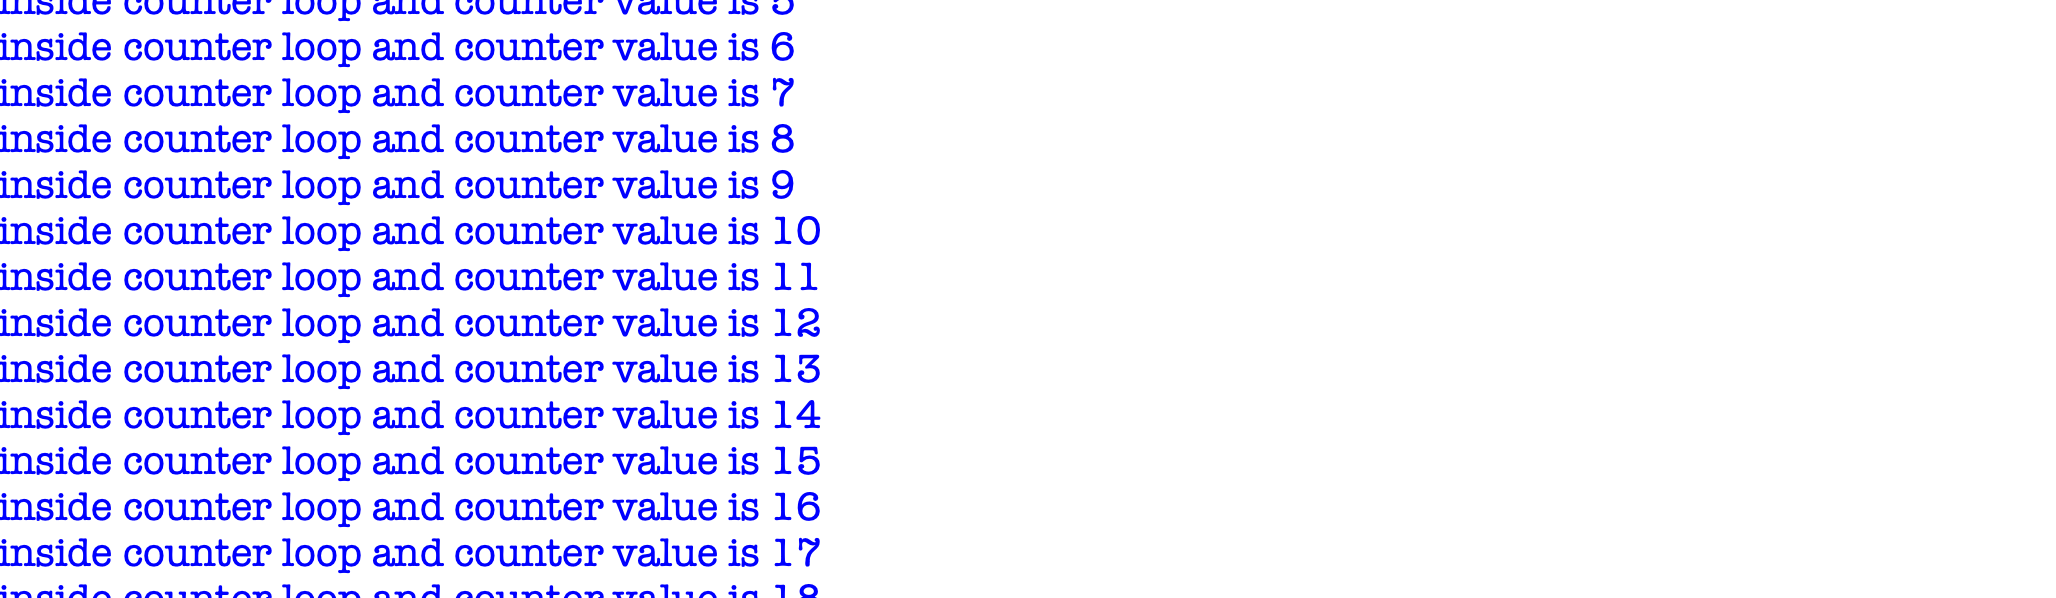
\includegraphics[width=17cm]{screen_shots/loop_counter.png}
	\caption*{Section of the output}
\end{figure}

\lstinputlisting[language=Python, caption=Python example]{loop_condition.py}
\begin{figure} [!h]
	\centering
	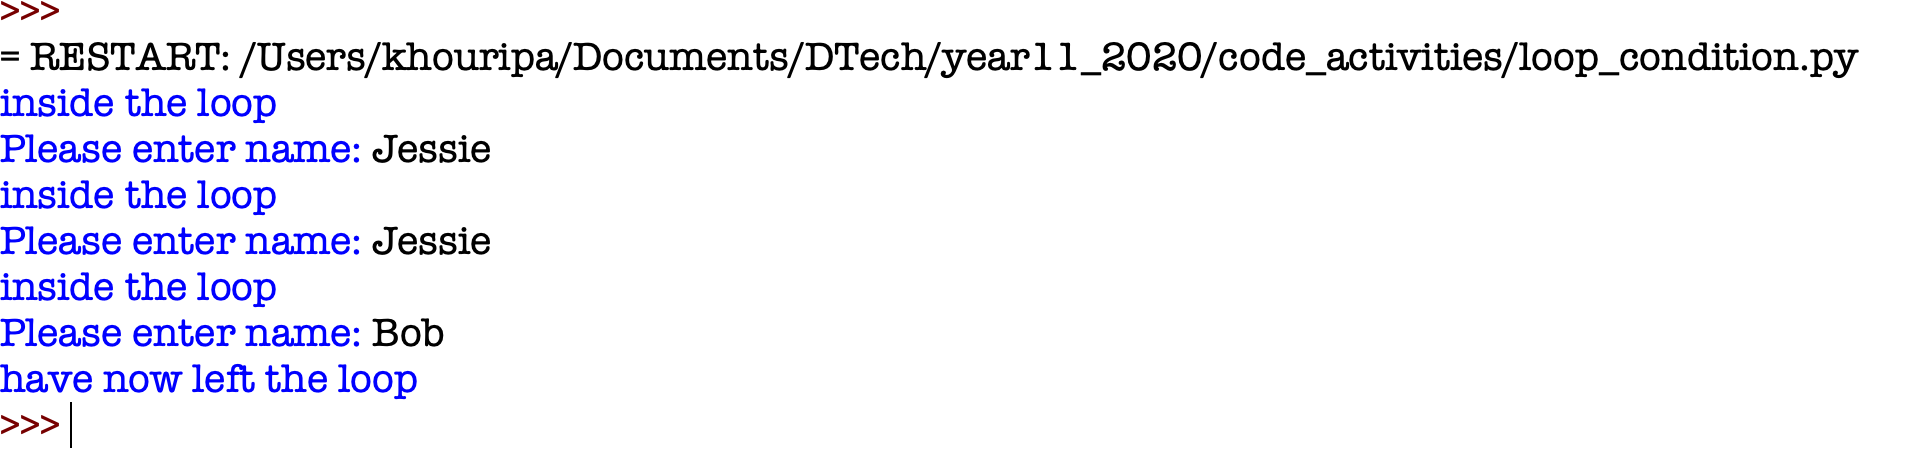
\includegraphics[width=17cm]{screen_shots/loop_condition.png}
\end{figure}
\newpage
\lstinputlisting[language=Python, caption=Python example]{loop_continue.py}
\begin{figure} [!h]
	\centering
	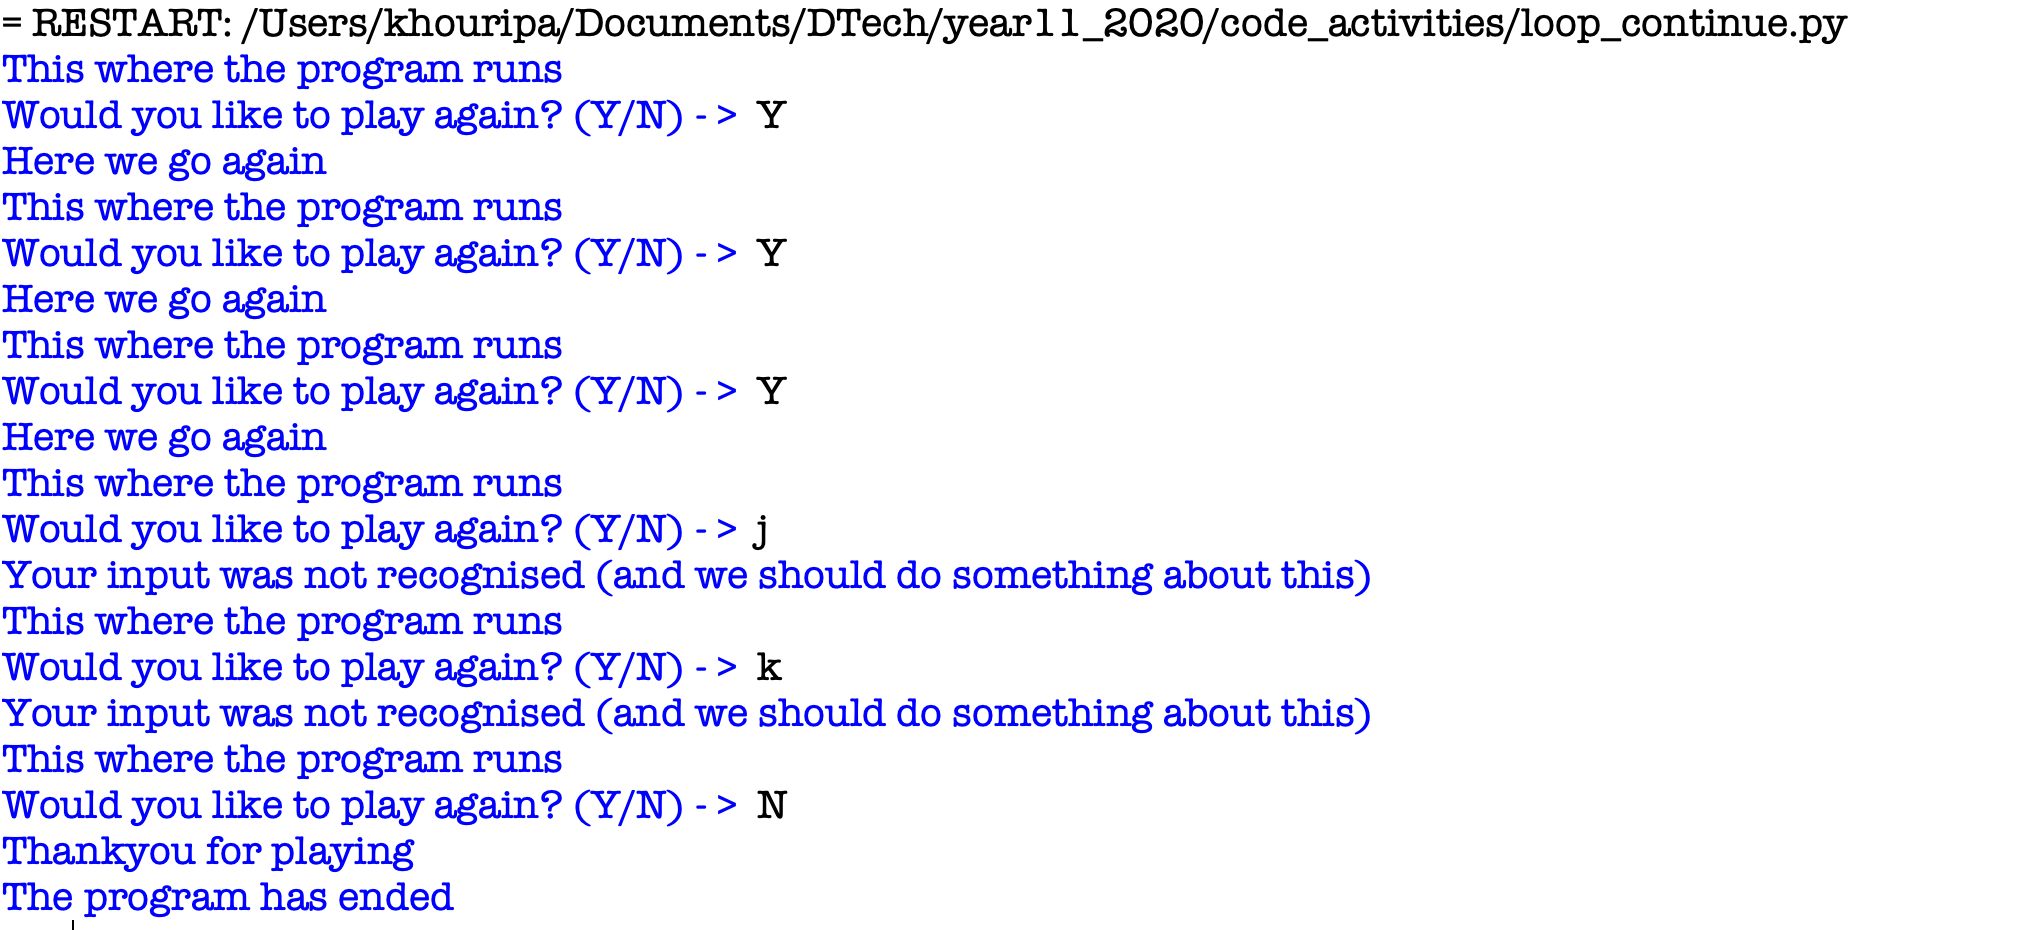
\includegraphics[width=17cm]{screen_shots/loop_continue.png}
\end{figure}
\newpage
\subsection{Activities - improving previously made programs}
Take the Dinner Order and/or the Higher Lower Program (make min = 1and max =100 ) and make a new version so that they can run more than once.\\
There is now considerable scope  for extension:\\
Consider:
\begin{itemize}
\item Dinner order prints out total cost of all orders when the program finishes (and/or total mains, deserts, drinks ordered)
\item Higher Lower feeds back the number of guesses that the user took to find the number. 
\item Higher Lower, user could choose number of guesses that they need
\end{itemize}

\begin{figure} [!h]
	\centering
	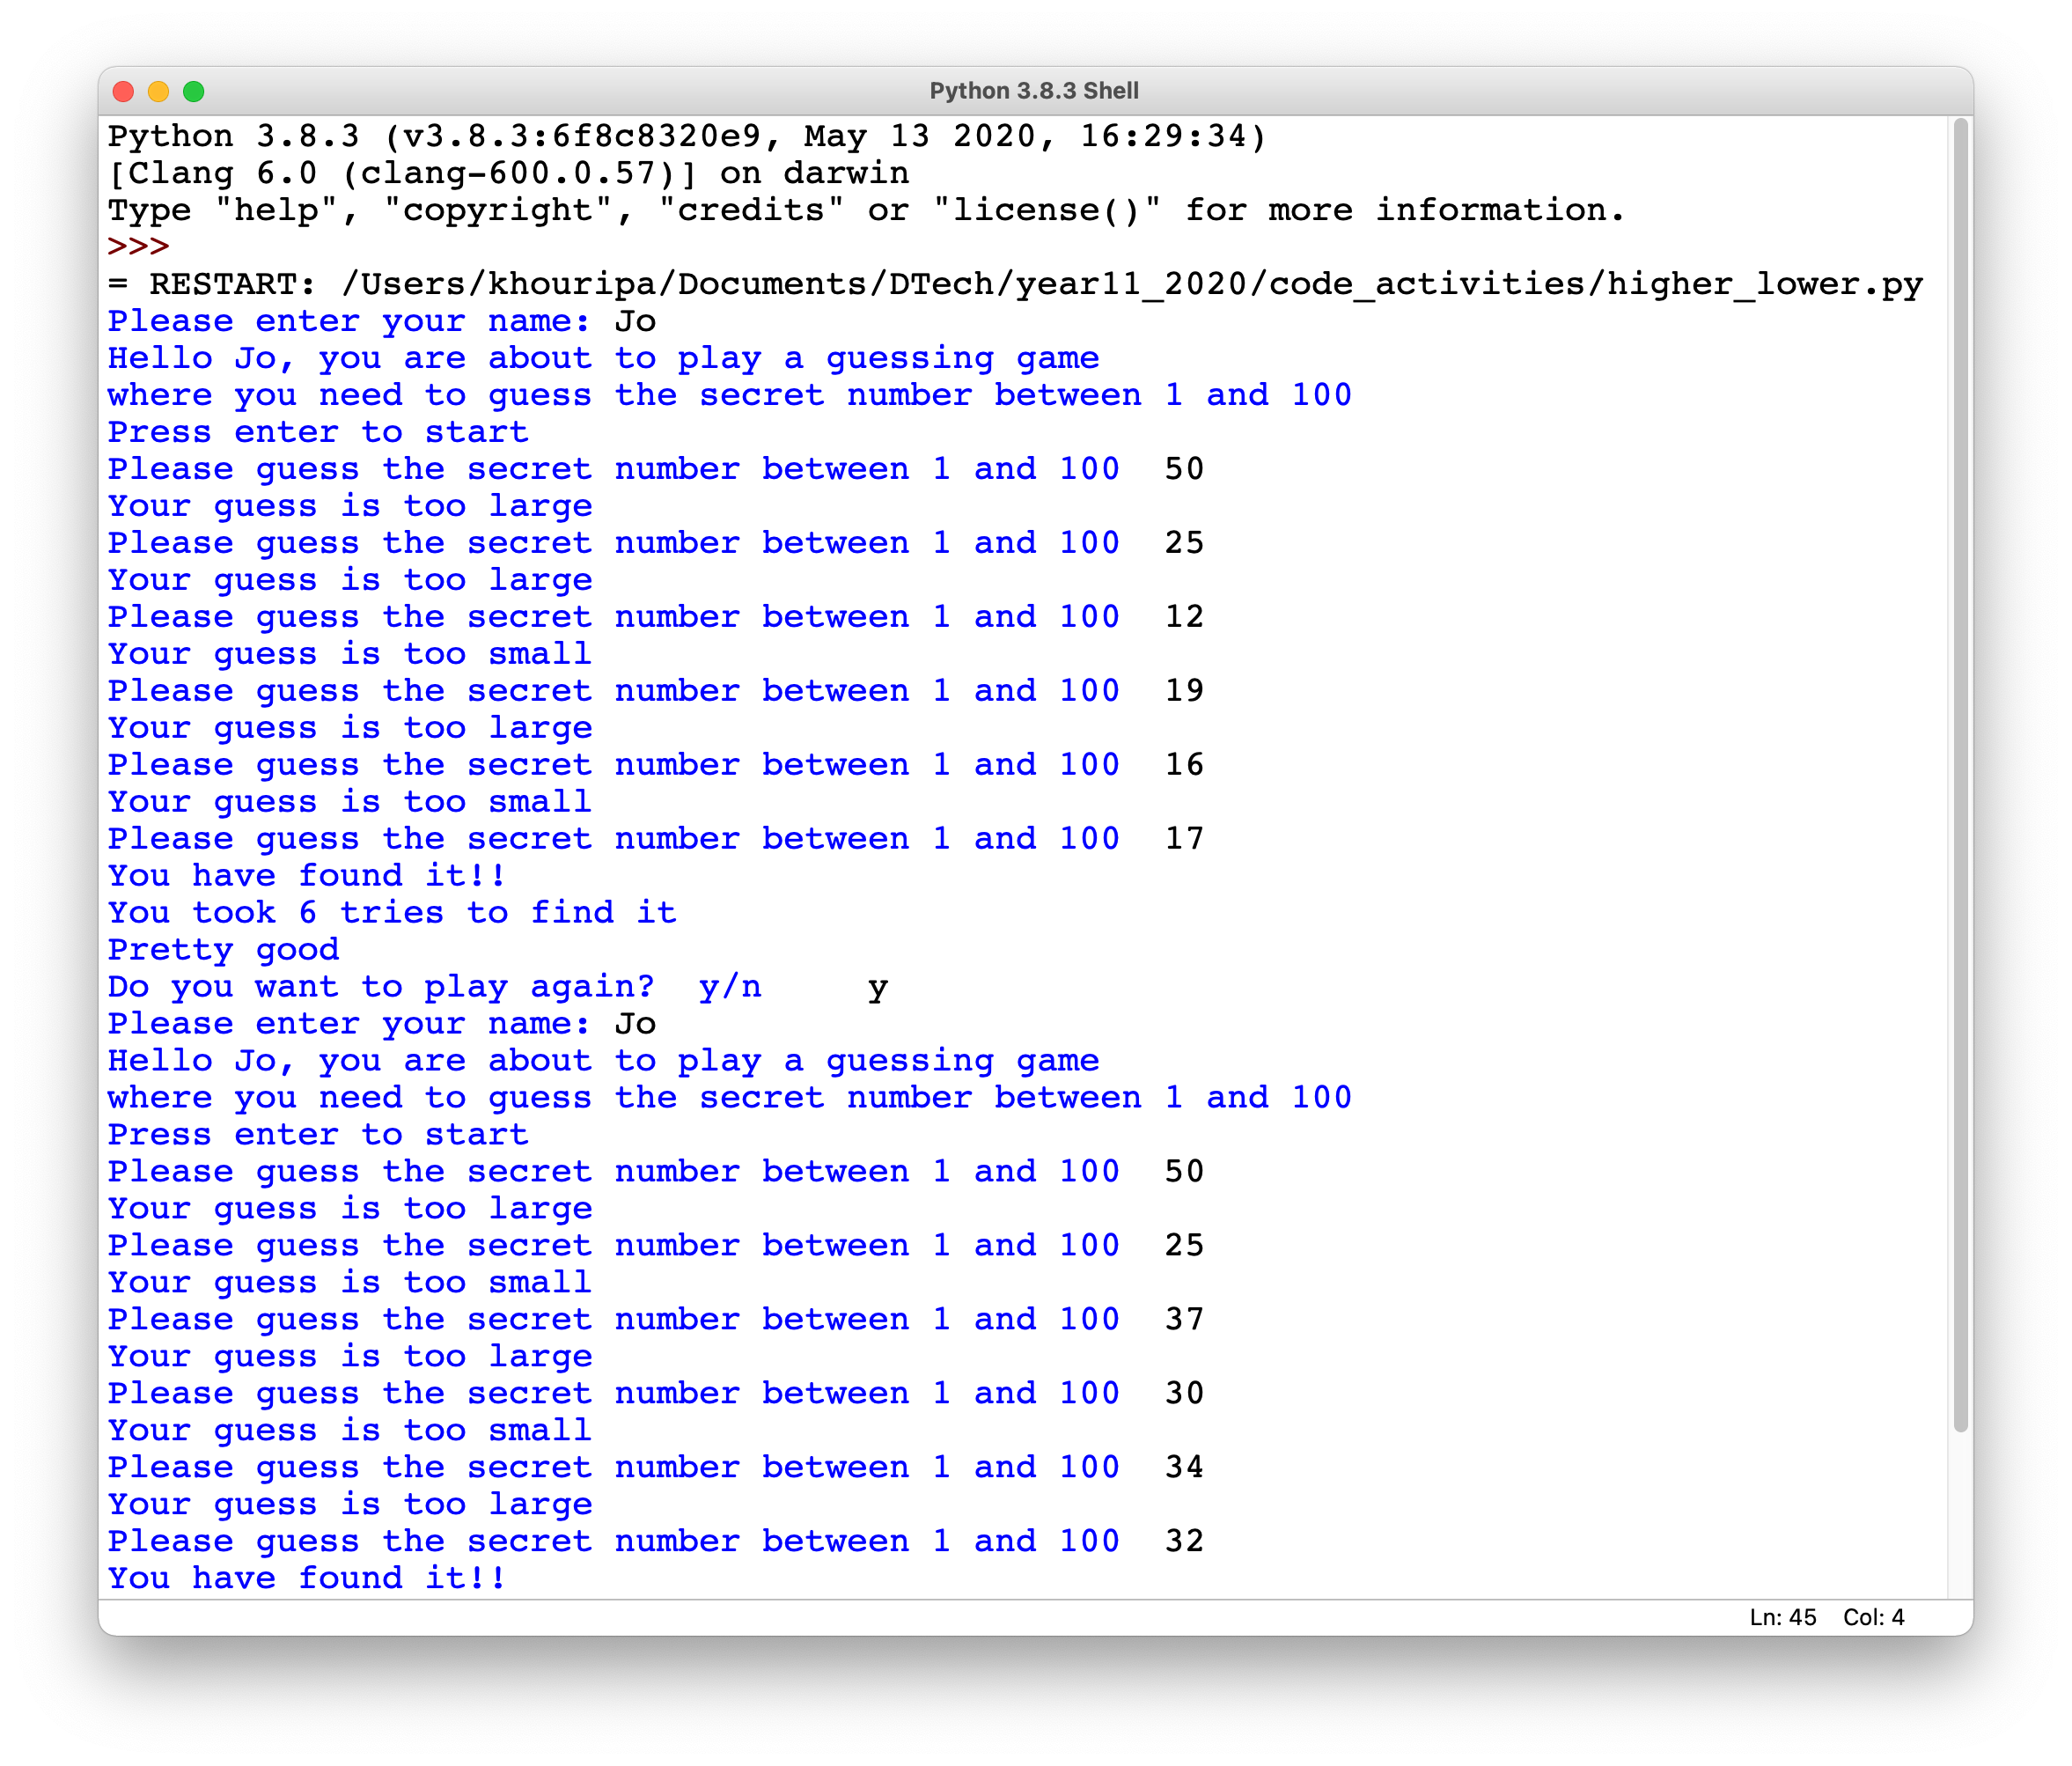
\includegraphics[width=15cm]{screen_shots/higher_lower_play.png}
	\caption*{Greater less equal, with loop and betting}
\end{figure}
\newpage
\begin{figure} [!h]
	\centering
	\includegraphics[width=17cm]{iterative_processes/higher_lower_loop_plan.pdf}
	\caption*{Psuedo code:Higher lower with loops}
\end{figure}
\lstinputlisting[language=Python, caption=Python example]{HigherLower/higher_lower_loop.py}

\newpage
\subsection{Higher Lower Game}
\begin{figure} [!h]
	\centering
	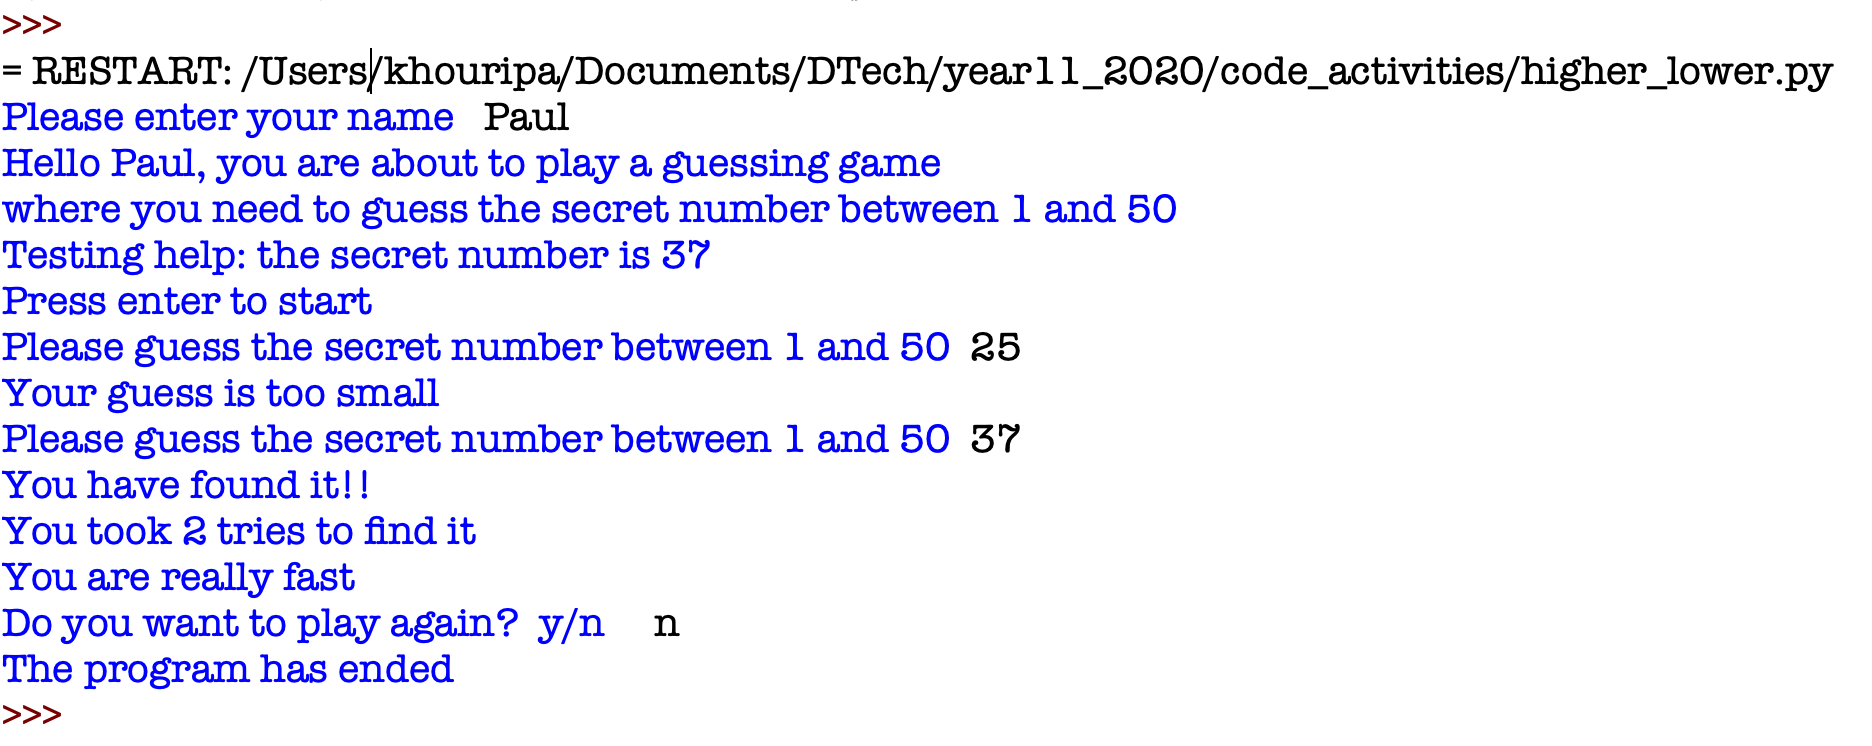
\includegraphics[width=17cm]{screen_shots/higher_lower.png}
\end{figure}
\subsubsection{Program}

\textbf{Scenario:}\\
You have a younger family member who loves the ‘higher / lower’ game so you decide to make a game that they can play whenever they want.\\
\hrule\vspace{0.5cm}
\textbf{Your game should:}
\begin{itemize}
	\item Ask for the user’s name (and address them by their name)
	\item Generate a ‘secret’ number between 1 and 100 and then ask the user to guess the number.
	\item Tell the user if their guess is ‘too high’ or ‘too low’.
	\item Then asks them to guess again (until they find the number)
	\item If the user correctly guesses the number, the game should congratulate them.
	\item Tell the user how many goes it took them to guess the number.
	\item If they don’t guess the number in 10 goes, they should be told that they have lost the game and the mystery number should be revealed.
\end{itemize}

\hrule\vspace{0.5cm}


\textbf{Improvements:\\ (do not worry about these until you have completed the main requirements)}:\\
Create small test programs to work out how to solve the problem before you include them in your next program version.
\begin{itemize}
	\item Allow the user to choose the lowest and highest number that will be used to generate the secret number between.
	\item Ideally the game should be set up so that users can’t guess the same ``wrong'' number twice ()This will require collecting a list of the guessed numbers).
	\item Either allow the user to choose the number of guesses or set a sensible limit based on the difference between the highest and lowest number.
	\item Keep track of the number of rounds played and the user’s scores.
	\item Improve the \textbf{usability} of the game by \textbf{validating} the user entry to make sure that it is appropriate.
\end{itemize}
\hrule\vspace{0.5cm}


\subsubsection{Planning, Developing, Testing}
\begin{itemize}
	\item \textbf{On paper} you need to break the big problem of making the program into a set of smaller sub-problems
\begin{itemize}
	\item If a problem looks tricky or there may be more than one way to solve it, you should make small test programs
\end{itemize}
\item Sketch out psuedo code for the main things you are going to make\\ ( ideally before you make it :) )
\item Don't create the program all in one go, build the simplest \textbf{version} you can. 
\begin{itemize}
	\item  Then test it and then plan and  build the next version. 
	\item After each version you should make some simple notes about what works, what could be improved , what the aim for the next stage is.
	\item Then plan, build and test the next \textbf{version}
	\item Repeat this process to \textbf{iteratively} develop the program.
\end{itemize}

\end{itemize}
%\textbf{Task:}\\
%As well as a working program , you need to provide evidence showing how the problem has been decomposed,  how the components have been developed and trialled, and of how they have been assembled and tested to create a final, working outcome.\\
%
%Decompose the problem (write down the decomposition on the template supplied)\\
%For each part of the problem, write (and test) each piece of code.  \\
%Before you write a piece of code, you should generate a quick test plan so that you can confirm that the code works correctly. \\
%Place your test plan and testing evidence on the supplied template.\\
%Combine your code into a fully working program\\
%Test and debug your program to ensure that it works for expected, boundary and unexpected values.\\
%Ask a friend / parent to play your game.  \\
%Watch them as they do this and make note of any changes that could be made to make the game easier to use\\
%Make the changes identified in the previous step\\
%Retest your game to ensure that it still works correctly\\
%
%\begin{itemize}
%	\item Outline / Decomposition:\\
%	Break the problem down into parts. \\
%	Clearly communicate the things you will need to be able to do, to make the program work.\\
%	Provide clear evidence of the Decomposition (diagrams or lists)
%	\item Build relevant test files (version 0 files) to solve/explore coding problems.  
%	\item Component Testing (happens after the Decomposition and at any other relevant time)\\
%	Show that you have tested each component. \\
%	You should have a test plan (how do you know it is working properly) and then screenshot proof for each component.  \\
%	You should also include notes that justify the major decisions you made.
%	\item Version Log\\
%	Log your different versions HigherLower-v1, HigherLower-v2, etc. (each of these is an iteration)
%	Include a brief description of what that have achieved.
%	\item Version Testing\\
%	Please show testing for your assembled outcome below.  
%	This should include a test plan followed by screenshot proof
%	Clearly communicate how you can verify that the version is working properly.
%	\item Usability Testing\\
%	Try the program out on someone else and make notes or video etc.
%	Write a list of things improvements which need to be made based on your usability testing.  Then write down what you changed.
%	\item Post Usability Test…\\
%	Show that your post usability testing program works correctly
%	Social and End User Considerations…
%	\item General Evaluation:\\
%	How good is may program? What can I do to improve it?
%	Repeat the relevant parts of the above process
%\end{itemize}
\newpage
\begin{figure} [!h]
	\centering
	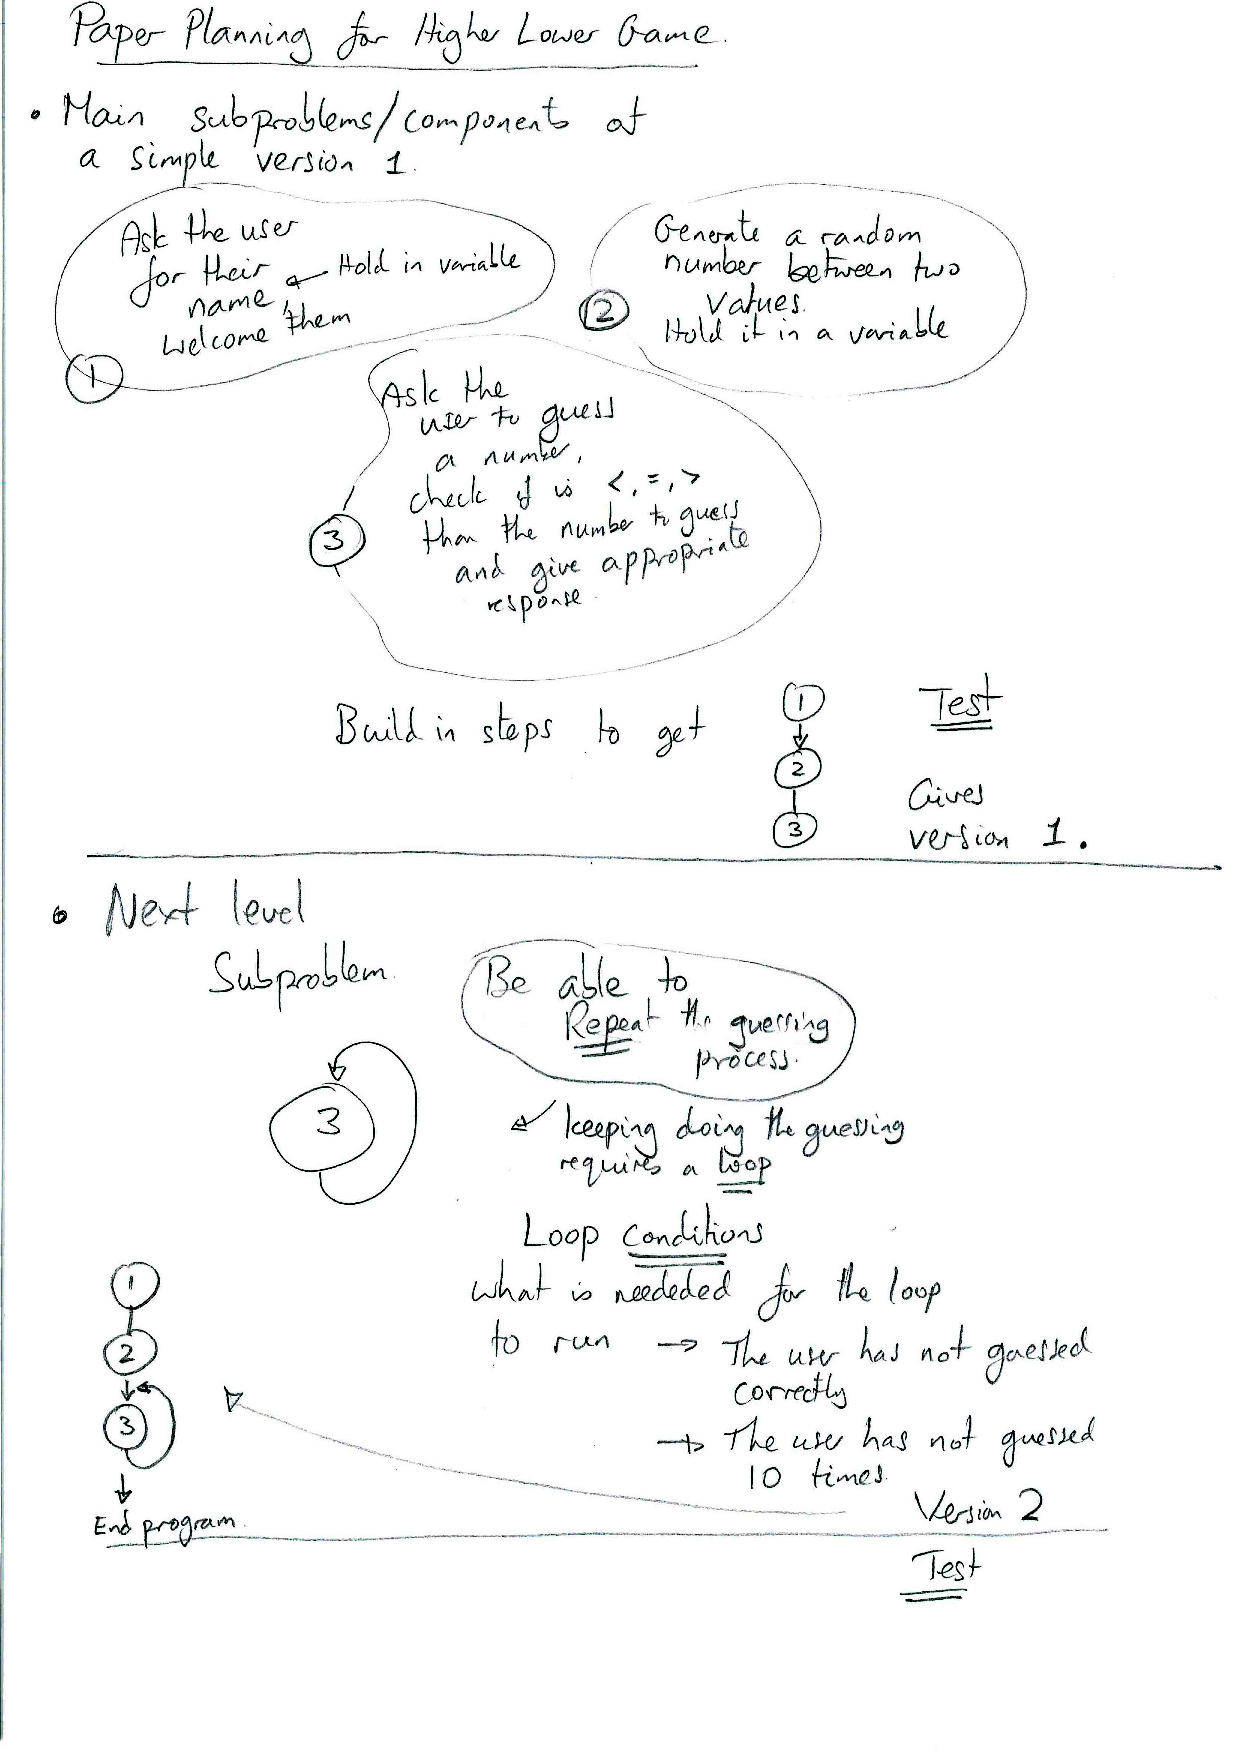
\includegraphics[width=17cm]{iterative_processes/higherlowerplanning-1.pdf}
\end{figure}

\newpage
\begin{figure} [!h]
	\centering
	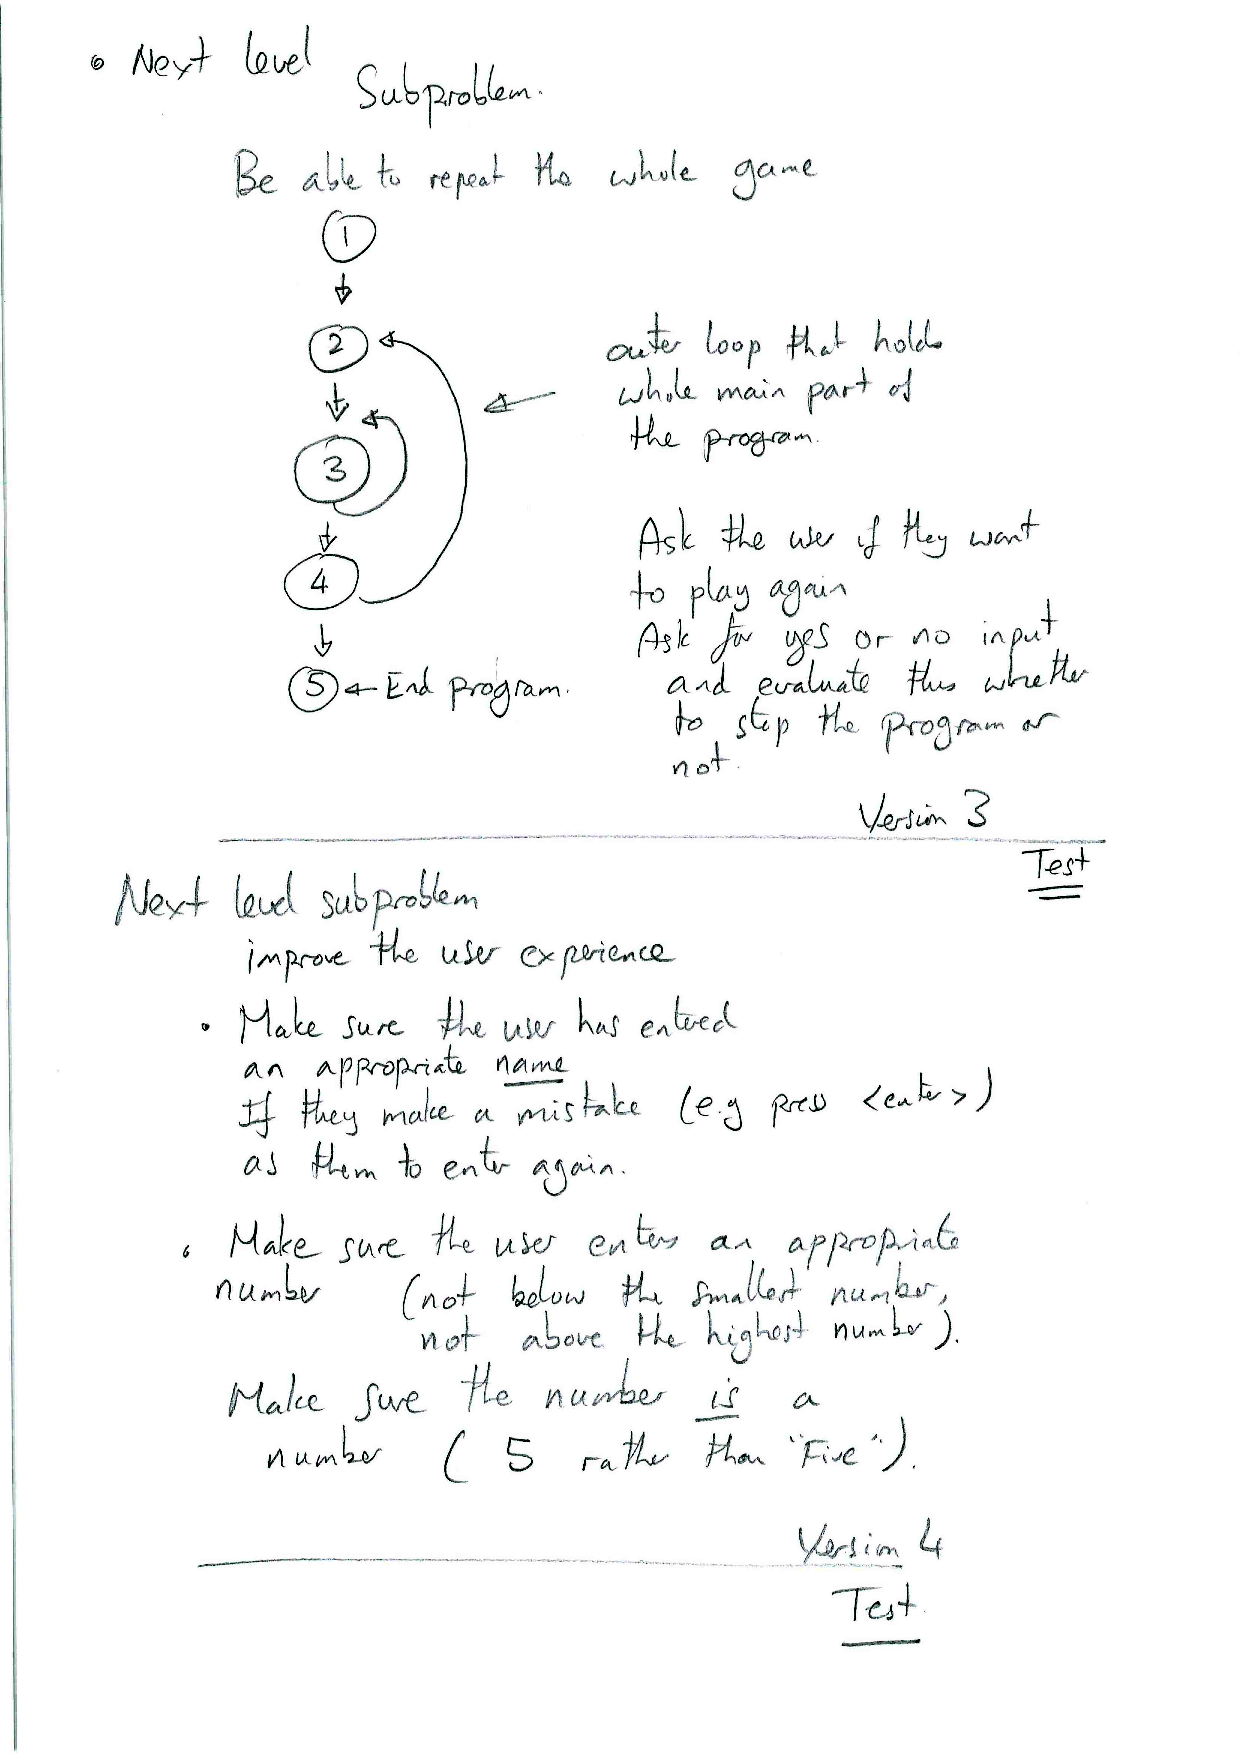
\includegraphics[width=17cm]{iterative_processes/higherlowerplanning-2.pdf}
\end{figure}



\newpage
\section{Functions}
Functions allow use to package up blocks of code in a separate place and the re-use them whenever we need them.\\
\begin{itemize}
	\item A function is made using the ``def'' statement
	\item It is then given any logical name (no spaces, no numbers in the name)
	\item A function has values that can be given to it. These are placed as variable names in the round brackets after the name.
	\item we can then use these values ``inside'' the function
	\item the function can be ``called'' (made to do its thing) by writing the function name in the main body of code (with values)
	\item functions can send values back to the main part of the program using the ``return'' statement.
\end{itemize}
\lstinputlisting[language=Python, caption=Functions]{maths_functions.py}
\begin{figure} [!h]
	\centering
	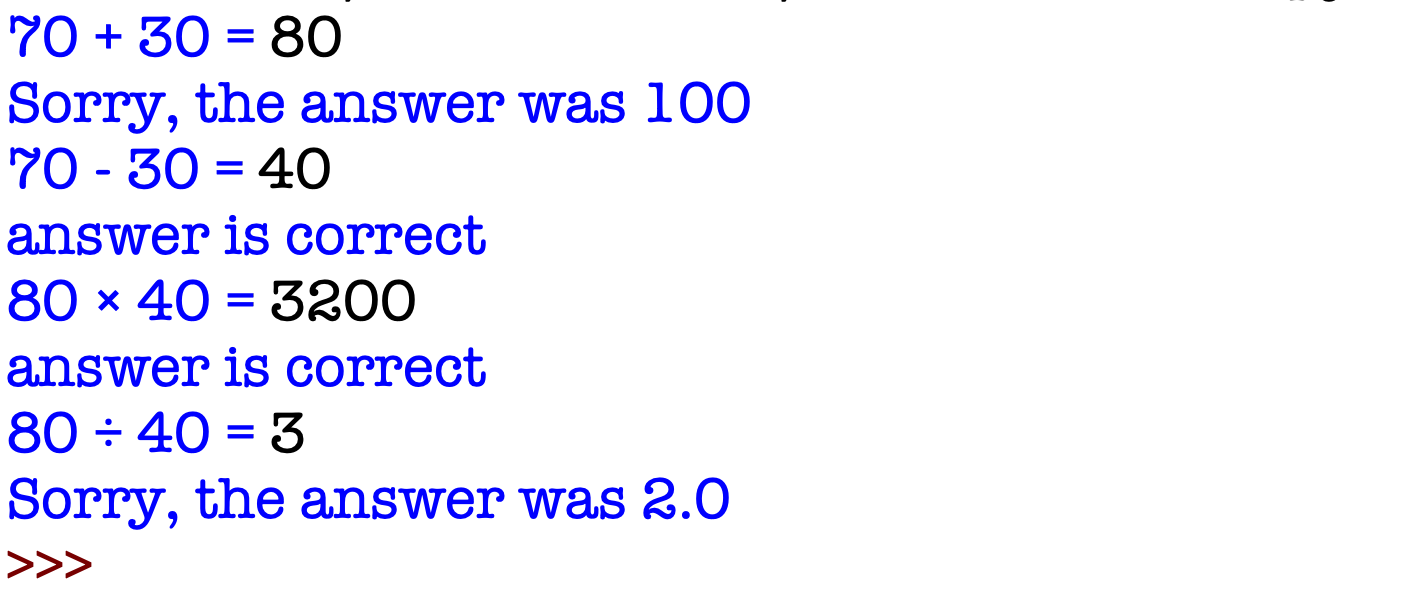
\includegraphics[width=15cm]{screen_shots/maths_functions_cap.png}
	\caption*{Functions output}
\end{figure}
\newpage
\subsection{Developing the maths functions into a little quiz}
\textbf{Idea 1:}
\begin{itemize}
	\item The quiz asks 4 maths questions and at the end gives the number correct (the score) and the number of questions asked
\end{itemize}
\textbf{Idea 2:}
\begin{itemize}
	\item (A loop would be nice.)\\
	Just using the adding function, the quiz asks 5 questions, and the numbers in the addition are \underline{randomly} chosen. \\
	The score is printed out as well as the total number of questions.
\end{itemize}
\textbf{Idea 3:}
\begin{itemize}
	\item The quiz asks 6 questions. Whether it will be a addition, subtraction, multiplication or division question is \underline{randomly} chosen.\\
	
\end{itemize}

\newpage
\section{Validation}
When a user is making an input they may make an error and enter an \textbf{invalid} input.\\
This is an input that the program is not expecting:\\
Examples include:
\begin{itemize}
	\item Entering a string instead of a number (such as ``Two'' or ``Tracy'' when the program is expecting an integer or float).
	\item Entering nothing or a single letter , when the program wants a full name.
	\item Entering a letter ``outside of bounds'' (For example: the program expects one of A,B,C,D and the user enters F)
	\item Entering a number outside of bounds (For example, the program expects a number between 1 and 10 and the user enters 11).
	\item The program expects a single letter (``y'' or ``n''), but is given a word (``Yes'', ``No'').
	\item The program expects a capital letter (``A'') and is given a lower case letter (``a'').
\end{itemize}
Some of these entries can cause a program crash or just lead to poor ``performance'' of the program (for example: rejecting a user entry when what the user intended was valid).\\
The aim is always to make the program perform as well as possible and to be \textbf{User Friendly}.\\\\
To manage this \textbf{Usability} we need to \textbf{Validate} the user input.\\
This means one or both of two things:
\begin{itemize}
	\item If the user input is invalid, communicate the problem to the user and ask the user again for the entry
	\item Evaluate and possibly alter the user entry, so that its meaning is not changed but that it is formatted in a way that program expects. (An example of this is changing ``A'' to ``a''. \\ In this case the user does not need to be informed)
\end{itemize}


\newpage
\subsection{Integer Validation}
Consider an input request ``How many hamburgers would you like to order?''\\
\begin{itemize}
	\item We would expect this to be an integer with a value of 0 or more.
	\item Most likely we would like to ``operate'' on this later in the program (for example: multiply it by the cost of the hamburger to get a total price)
\end{itemize}
The input is always read as a string, so we need to cast the input to an integer.
\lstinputlisting[language=Python, caption=Python example]{validation_int_1.py}
This works properly \underline{assuming} the user enters a \underline{valid} input.\\
This is assumption is not good enough, and we need to deal with situations like the user entering $<$Enter$>$ or 3.5 or ``six''.\\
If they do, we get a program crash:
\begin{figure} [!h]
	\centering
	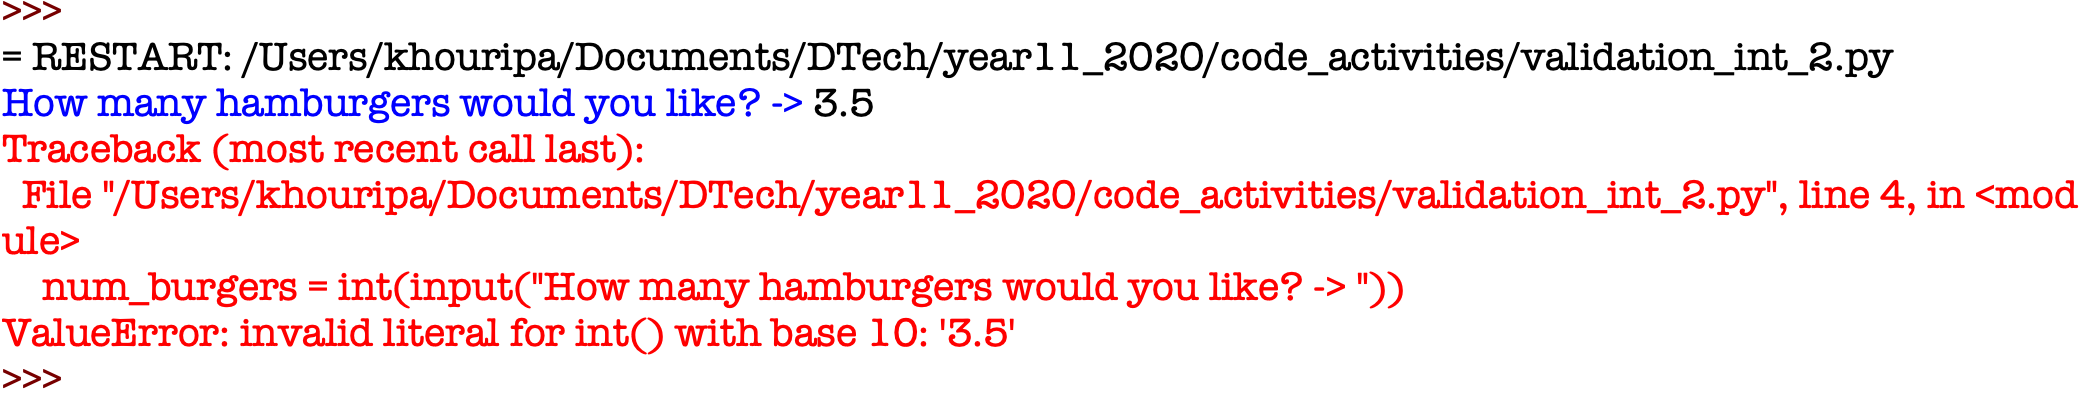
\includegraphics[width=17cm]{screen_shots/validation_int_1.png}
\end{figure}
To manage integer casting, we need a ``try except'' statement. This gets the program to do a check before accepting the cast.\\
The ``except ValueError'' will run if the input is not an integer.
\lstinputlisting[language=Python, caption=Python example]{validation_int_2.py}
\begin{figure} [!h]
	\centering
	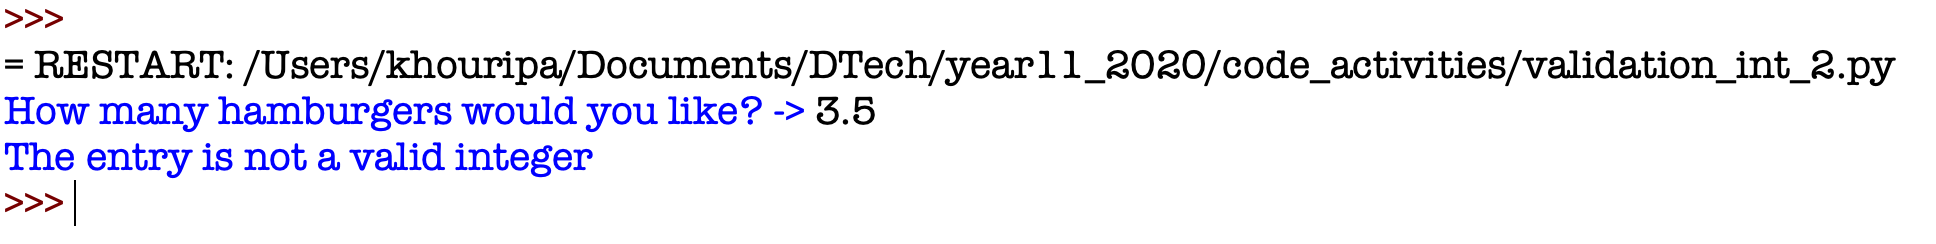
\includegraphics[width=17cm]{screen_shots/validation_int_2.png}
\end{figure}
This partly fixes the problem, but we still don't have an acceptable value for the number of hamburgers.\\
So we need to ask the user again for an input and if we want to ask again (and maybe again ....) we need a loop:

\lstinputlisting[language=Python, caption=Python example]{validation_int_3.py}
\begin{figure} [!h]
	\centering
	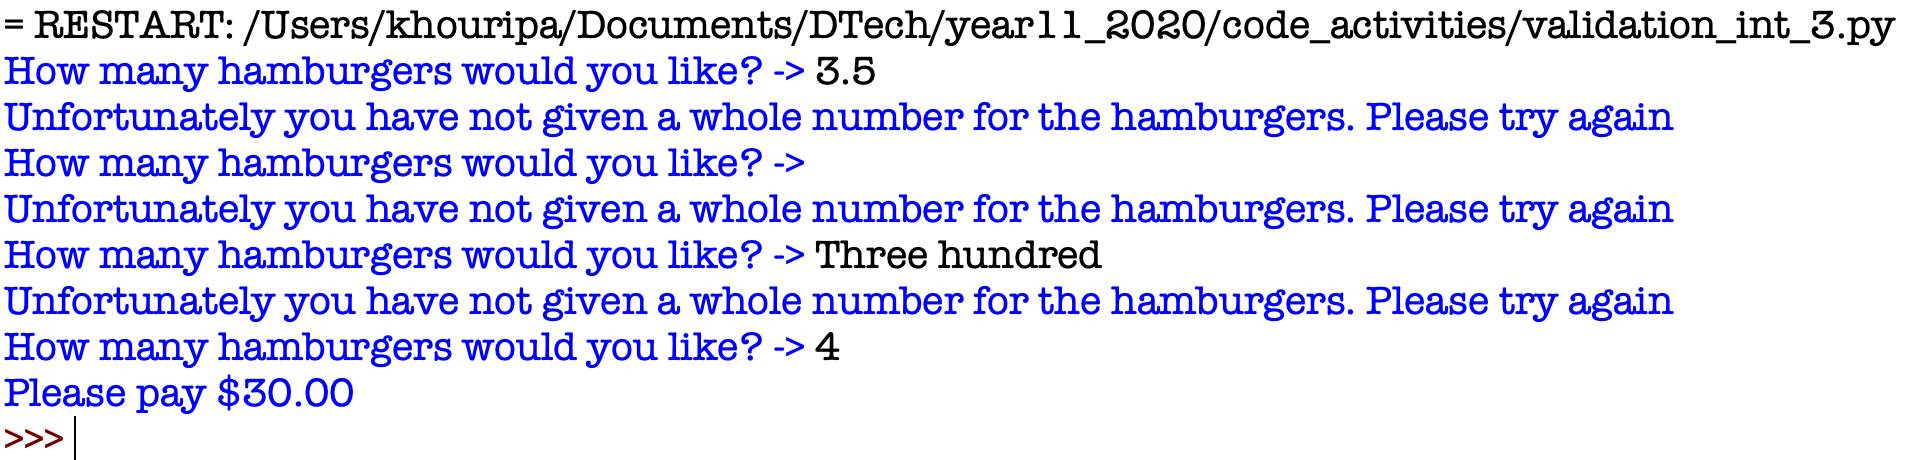
\includegraphics[width=17cm]{screen_shots/validation_int_3.png}
\end{figure}
 We still have a problem that the program accepts negative numbers:
 
 \begin{figure} [!h]
 	\centering
 	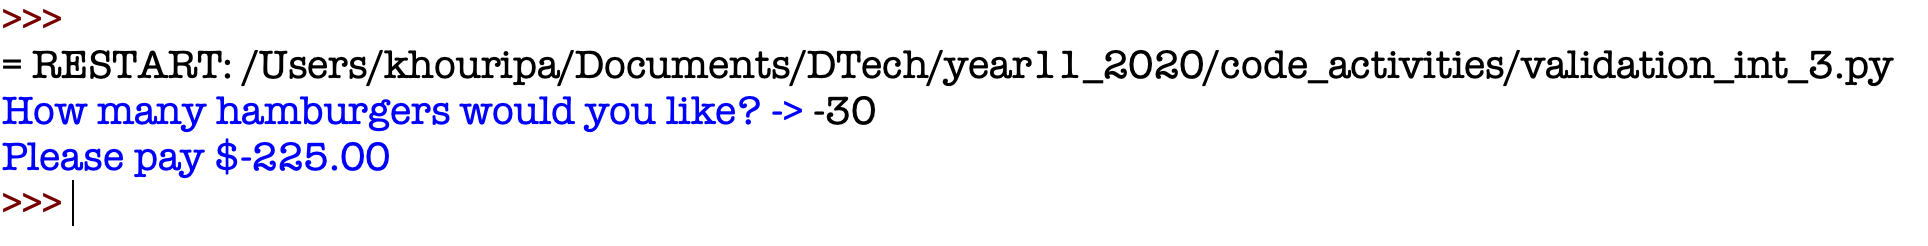
\includegraphics[width=17cm]{screen_shots/validation_int_3_neg.png}
 \end{figure}

So we can extend the the validation loop
\lstinputlisting[language=Python, caption=Python example]{validation_int_4.py}
 \begin{figure} [!h]
	\centering
	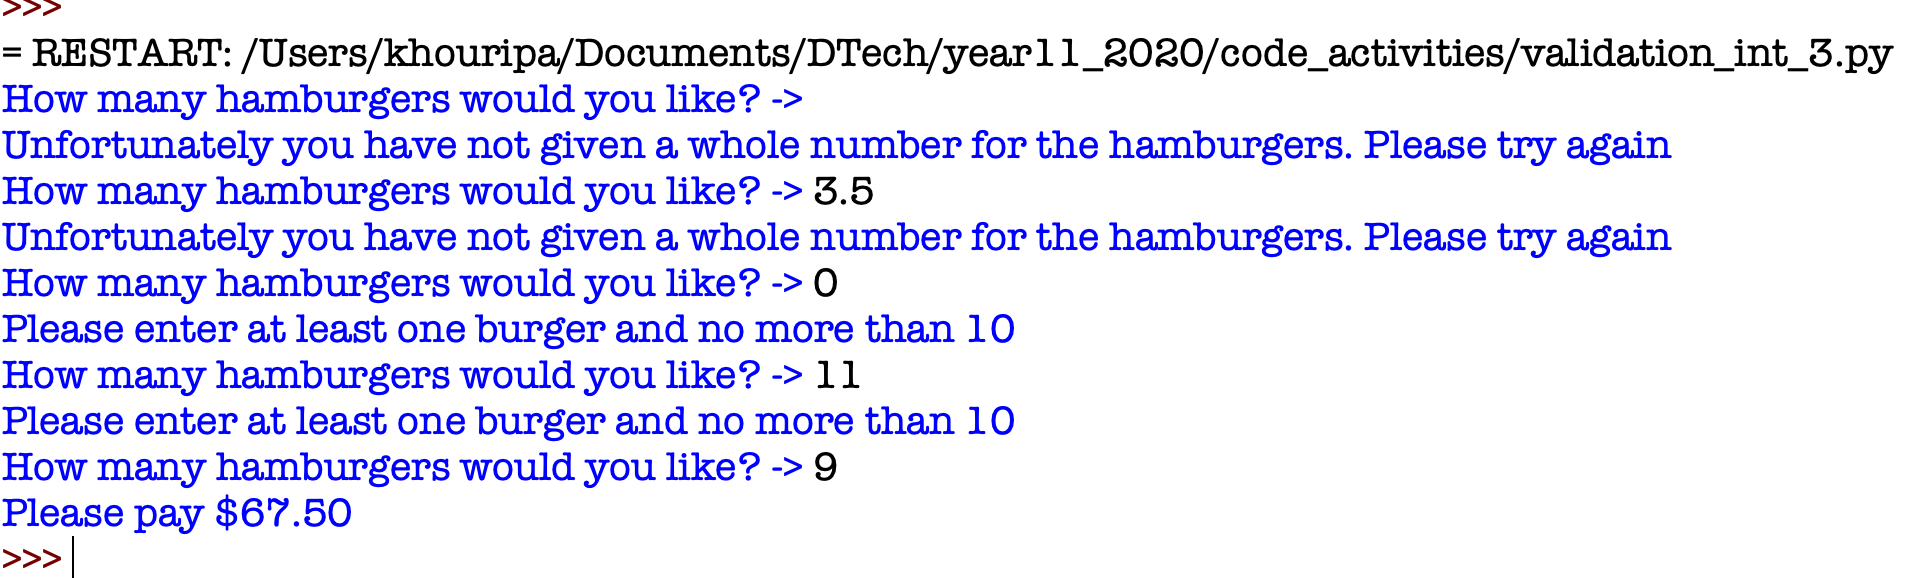
\includegraphics[width=17cm]{screen_shots/validation_int_4.png}
\end{figure}
\newpage
 \subsection{String Validation}
 If we require a name, we still need to check that we are getting something acceptable.\\
 A simple validation can be to check that the entry has at least 2  characters and no more than (maybe) 20 (what do you think is the longest number of characters that can be in a name?).
 
 \lstinputlisting[language=Python, caption=Python example]{validation_name.py}
 \begin{figure} [!h]
 	\centering
 	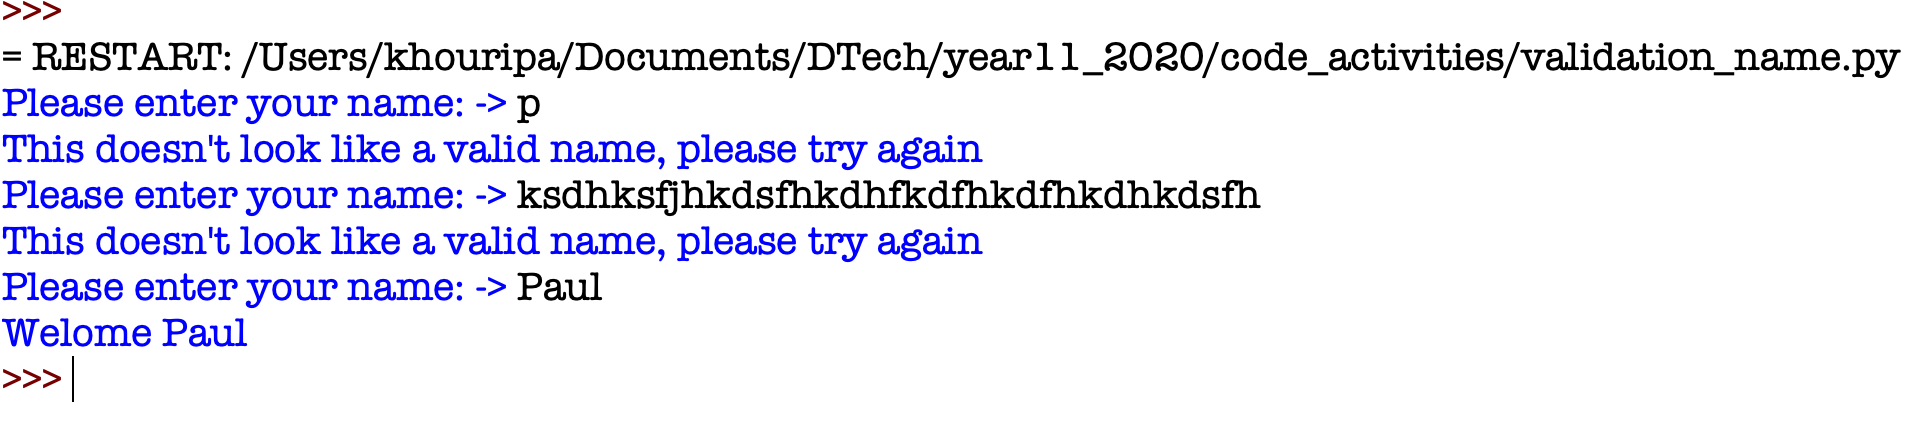
\includegraphics[width=17cm]{screen_shots/validation_name.png}
 \end{figure}

This validation checks that the characters in the name are all acceptable (i.e no numbers or special characters).\\
It does this by checking each character in the name against a list of characters than are acceptable.

 \lstinputlisting[language=Python, caption=Python example]{validation_name_1.py}
\begin{figure} [!h]
	\centering
	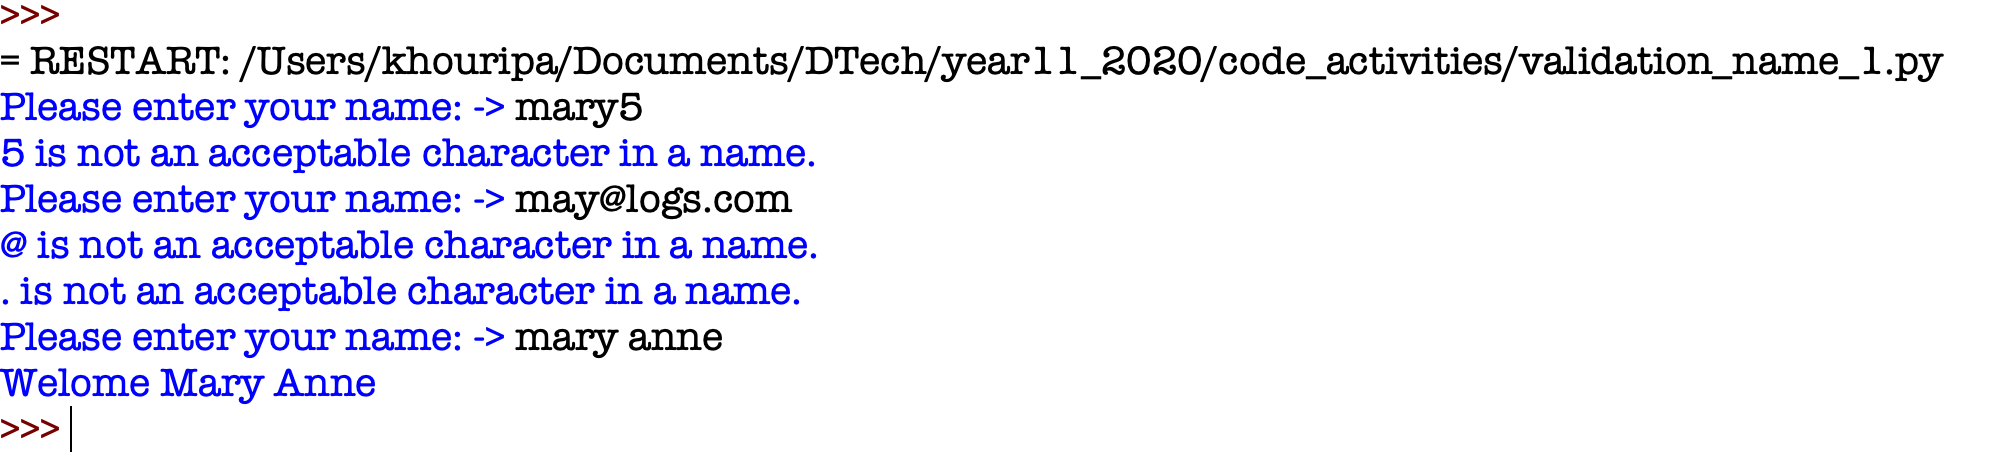
\includegraphics[width=17cm]{screen_shots/validation_name_1.png}
\end{figure}
 
 \begin{itemize}
 	\item Checking that strings follow an acceptable ``pattern'' is called ''regular expressions'' and this is outside of the scope of Level 1 (but we can explore options like in the code example).\\
 	\url{https://www.w3schools.com/python/python_regex.asp}
 	\item It is also a good idea to be familiar with ``string methods'' as they can be very useful.\\
 	\url{https://www.w3schools.com/python/python_strings_methods.asp}
 \end{itemize}




\newpage
\section{Lists}
Quite often we want to store a whole set of items (for example, names). Having a variable for each one is not very helpful (particularly if we want to add more names to the lists or remove some names).\\
Suppose we have a small class of 6 students and we want to store all of their names.\\
There names are: Agatha , Melinda, Harriet, Hine, Dandelion and Te Aroha\\
To create a list we use square brackets and commas.
\lstinputlisting[language=Python, caption=Python example]{list_base.py}
To manage lists, there are a large range of methods that can be used.\\
See the examples below.
\lstinputlisting[language=Python, caption=Python example]{list_base_1.py}
See also:
\begin{itemize}
	\item Python Lists:  \url{https://www.w3schools.com/python/python_lists.asp}
	\item Python List Methods: \url{https://www.w3schools.com/python/python_lists_methods.asp}
\end{itemize}



\section{Lists and Loops}
\subsection{Creating and modifying a class group}
\textbf{Scenario:}\\
Create a simple program that asks the user to enter the names for students in a class.\\
Once the names have been entered it prints out the names as a numbered list.\\
Extension:\\
One the names have been entered and listed, ask the user if they would like to modify or remove any of the names.
(and if they do allow them to do it)







\subsection{Lucky Unicorn Game}
\subsubsection{Program}
\textbf{Scenario:}\\
You have decided to create a fun game to raise money for the charity Doctors without Borders.\\ 
You will set up your computer at lunchtime and players will pay to play.  \\

\textbf{Here are the rules:}\\
Users pay an initial amount at the start of the game. 
\begin{itemize}
	\item The cost should be \$1 per round and users should press $<$enter$>$ to play.  
	\item The computer should then generate a token that is either a zebra, horse, donkey or unicorn.  
	\item This should be displayed to the user (as text). 
	\item If the token is a unicorn, the user wins \$5, if it is a zebra or horse, they win 50c and if it is a donkey then they don’t win anything. 
\end{itemize}
\hrule \vspace{0.5cm}

The maximum amount of money that students can spend on the game is \$10 per session. 
 \begin{itemize}
	\item The game should allow players continue / quit provided they have not lost all of their money. 
	\item  It should supply appropriate feedback so that the user knows how much money they have won / lost each round and how much money they have left.
\end{itemize}
\hrule \vspace{0.5cm}

Once students have no more money, the game should end (although players do have the option of quitting while they are ahead).\\

\hrule \vspace{0.5cm}


Variations (optional)
Once you have a working game, you are welcome to develop the outcome further.  \\
Here are some variations you could consider…
\begin{itemize}
	\item Change the tokens / context ( so rather than having zebra, horses, donkeys and unicorns the game could involve other items )
	\item Allow users to bet more than \$1 per round and adjust the pay-outs proportionally\\ 
(be careful to set up you game so that the house has a long term advantage)
\end{itemize}


\newpage
\subsubsection{Planning: Iterative Processes}
\begin{itemize}
	\item Break the problem down into parts (Draw some kind of diagram)
	\item Each of the parts can be called a ``component'' of the program or a ``sub-problem''.
	\item You need plan and test code for each of these ``sub-problems''.
	\begin{itemize}
		\item Ideally (and this must happen somewhere), you need to look at ``trialling'' different ways to solve the sub-problem), with the idea being that you can trial the different ways and choose the best (and also look to ways of improving). \\
		This needs to be captured in the planning documentation for the iterative processes assessment.
	\end{itemize}
	\item Combine your code into a fully working program (your first version)
	\begin{itemize}
		\item Test the program and document the test (gridded test plan)
		\item Write a short reflection on what works and what could be improved upon.
	\end{itemize}
\item Plan the next version 
\begin{itemize}
	\item Test the program and document the test (gridded test plan)
	\item Write a short reflection on what works and what could be improved upon.
\end{itemize}
\item Repeat this planning and testing process.
\item If new sub-problems appear , then work on them in the same way as referred to above
\end{itemize}
\newpage

\begin{figure} [!h]
	\centering
	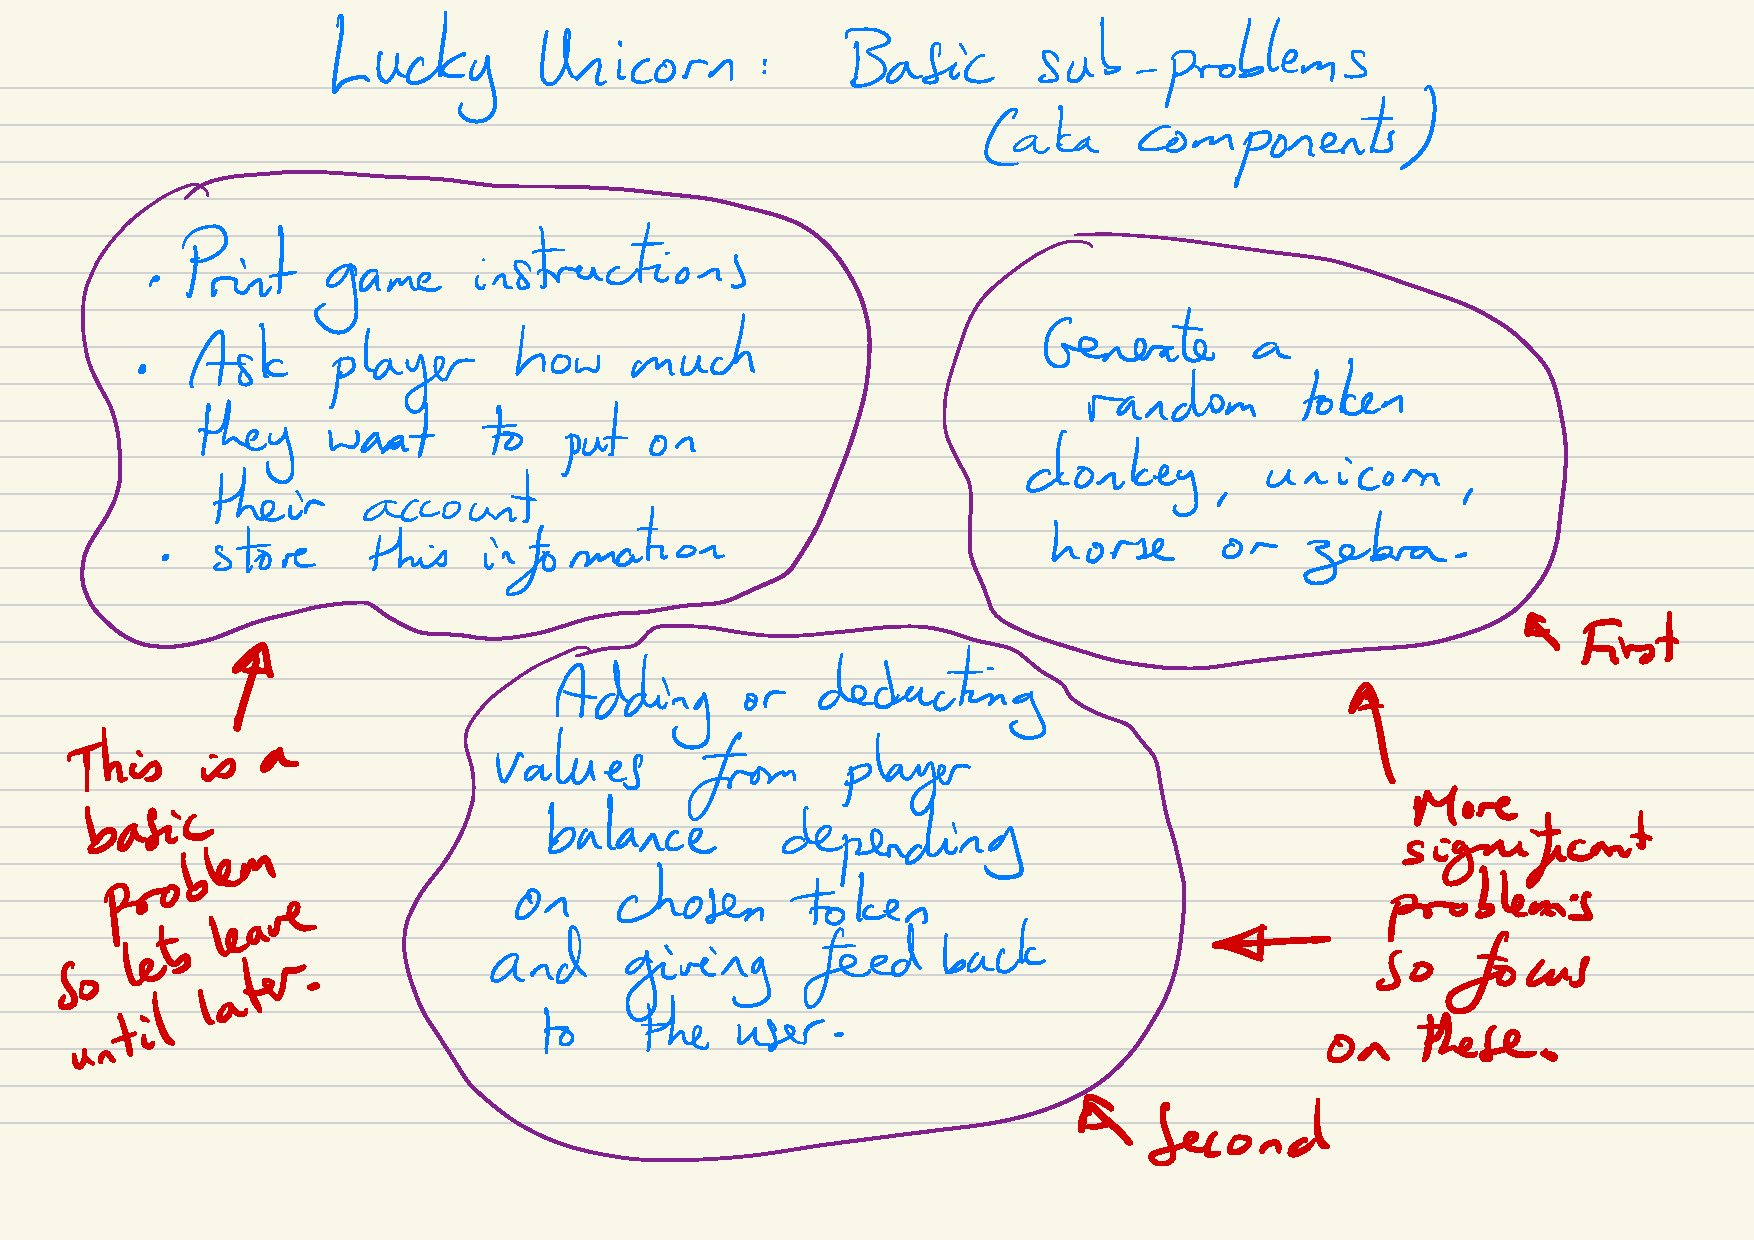
\includegraphics[width=15cm]{iterative_processes/Lucky_Unicorn_Sub_problems_1.pdf}
	\caption*{Breaking the problem down into components}
\end{figure}

\begin{figure} [!h]
	\centering
	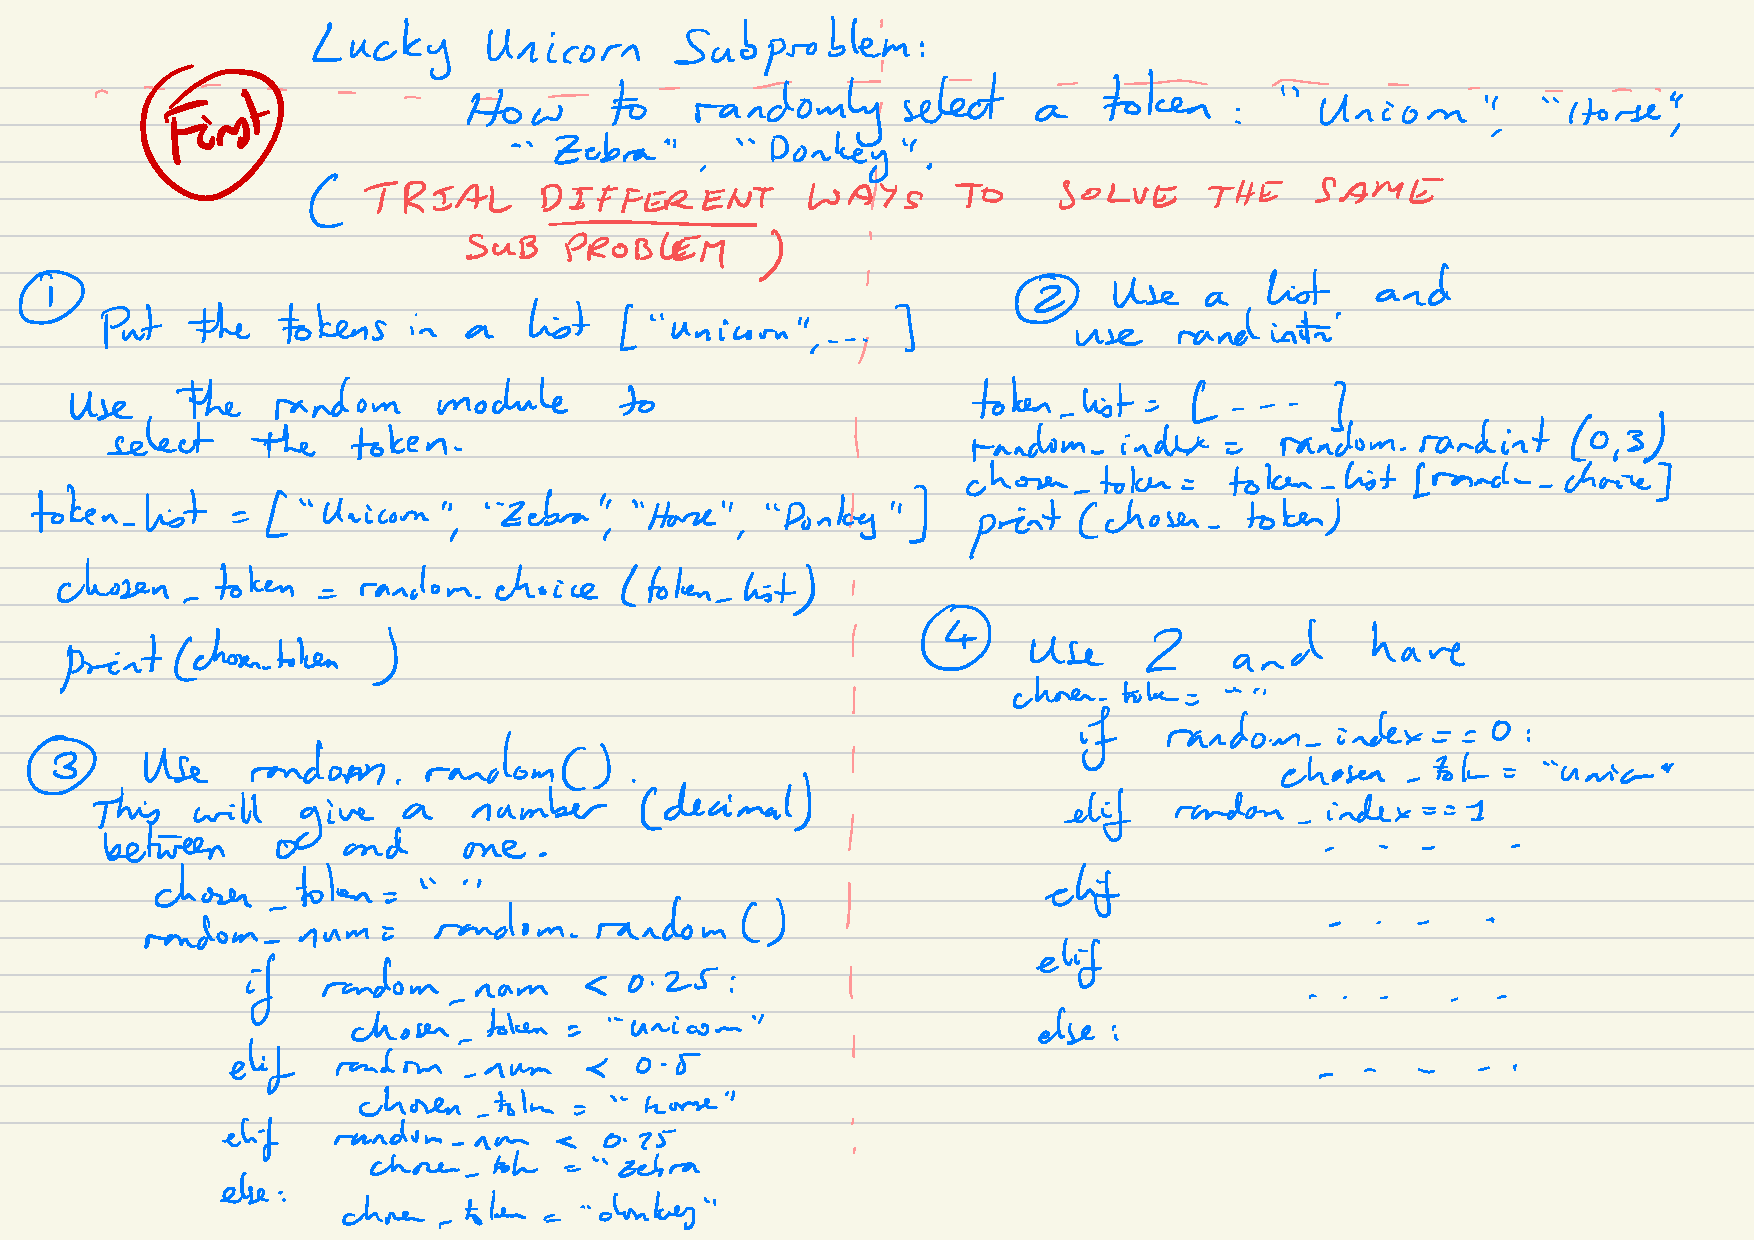
\includegraphics[width=15cm]{iterative_processes/Lucky_Unicorn_Sub_problems_2.pdf}
	\caption*{Planning options for the first sub-problem}
\end{figure}

\newpage

\begin{figure} [!h]
	\centering
	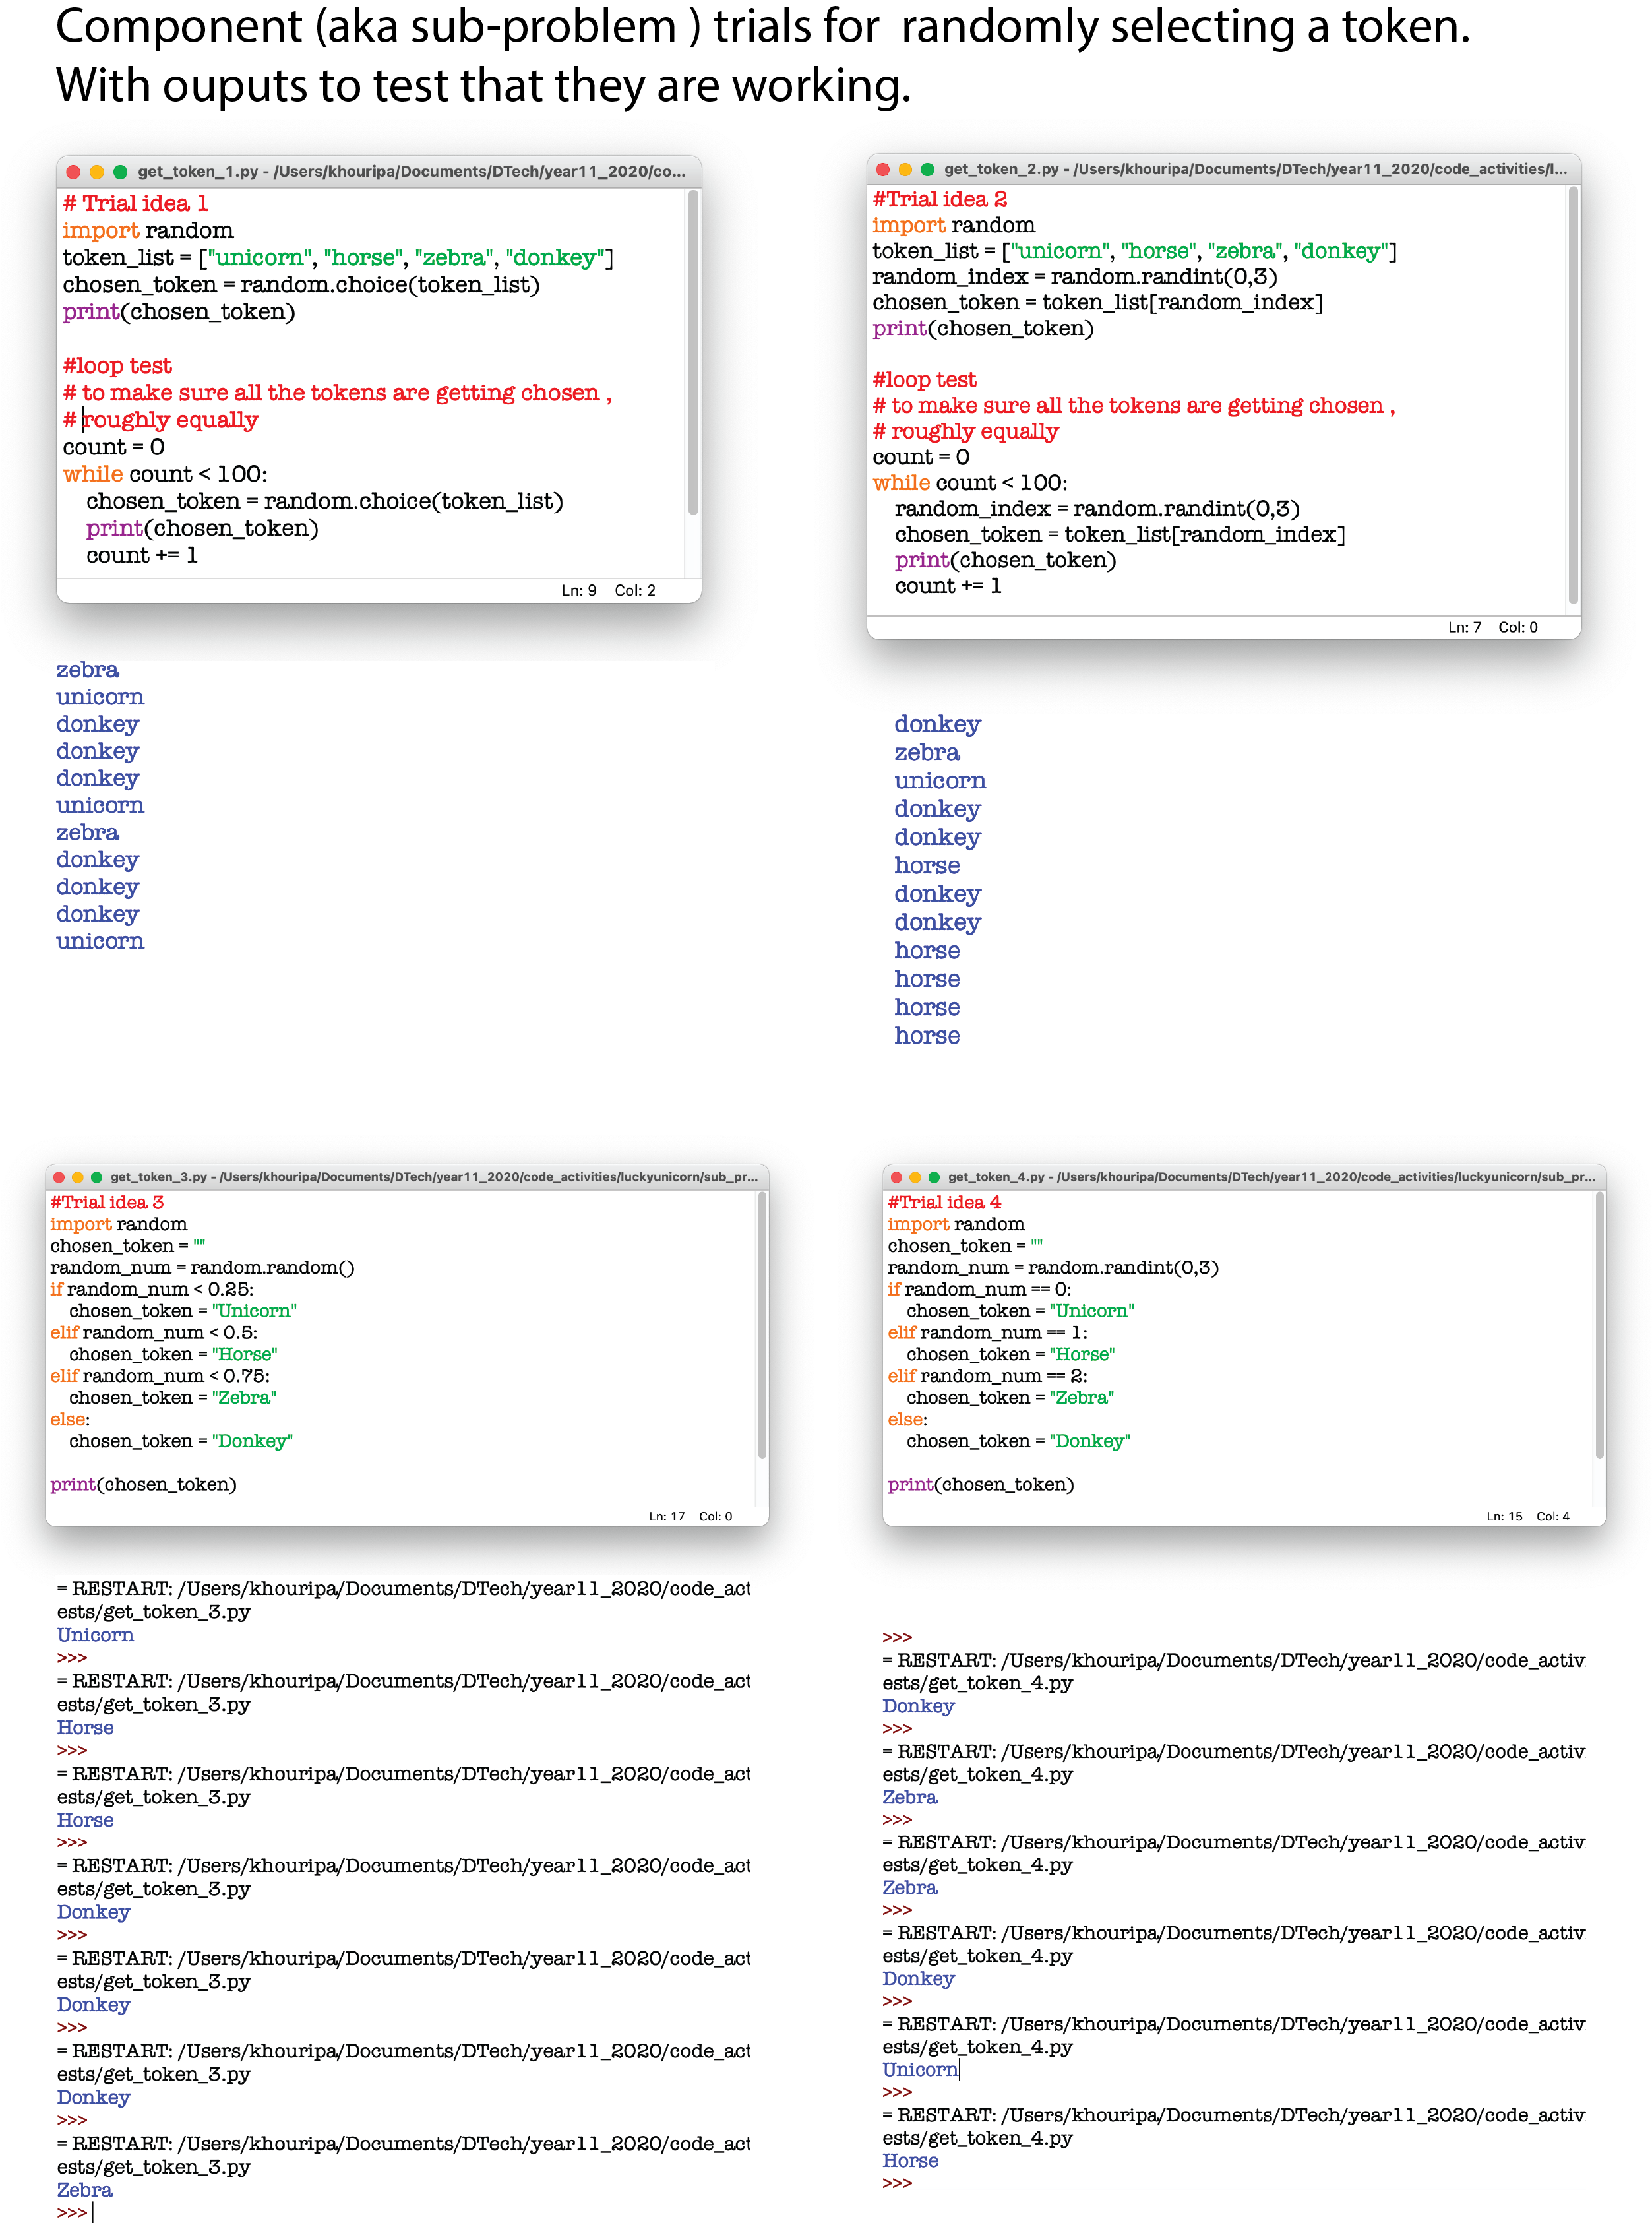
\includegraphics[width=17cm]{iterative_processes/sub_problem_trials.png}
	\caption*{Trialling different ways to solve the same sub-problem}
\end{figure}

\newpage

\begin{figure} [!h]
	\centering
	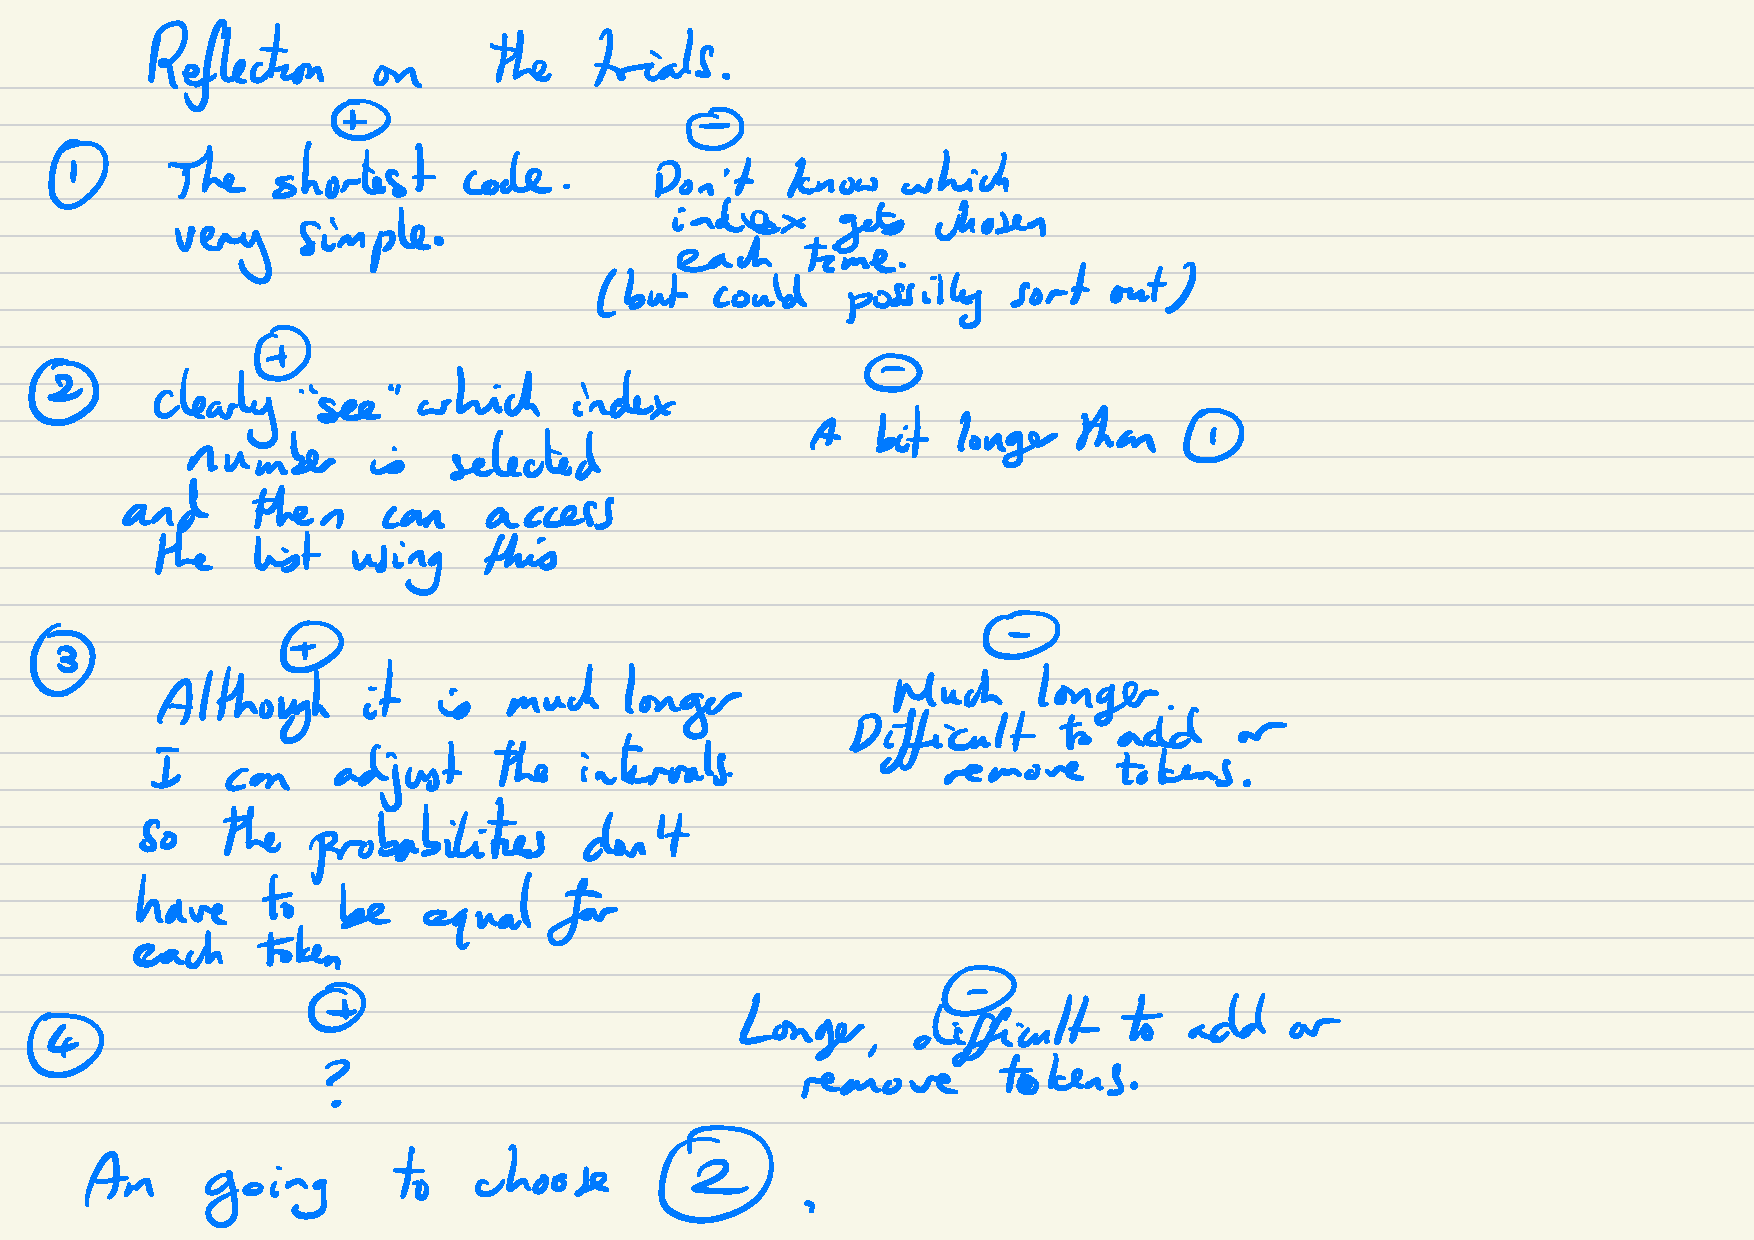
\includegraphics[width=15cm]{iterative_processes/Lucky_Unicorn_Sub_problems_2_a.pdf}
	\caption*{A reflection on the trials and a choice}
\end{figure}

\begin{figure} [!h]
	\centering
	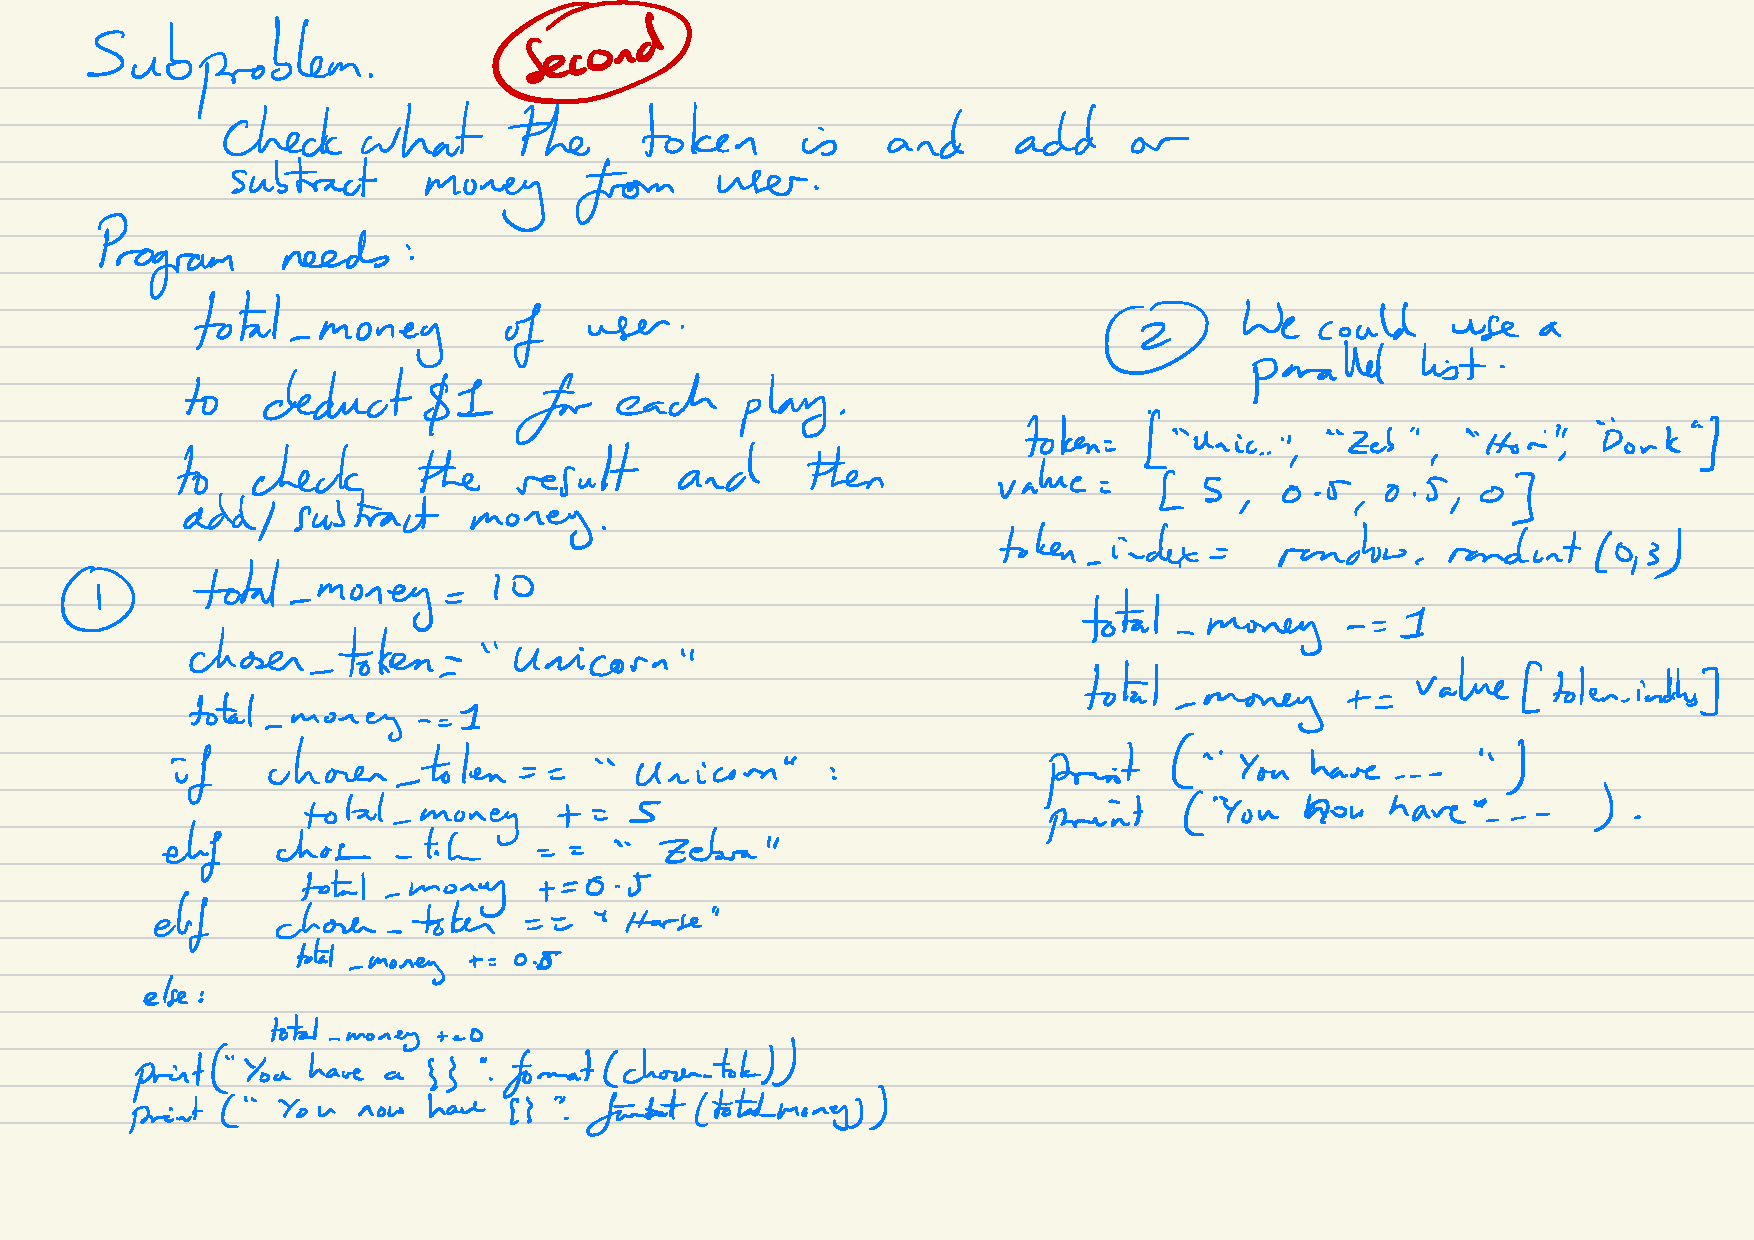
\includegraphics[width=15cm]{iterative_processes/Lucky_Unicorn_Sub_problems_3.pdf}
	\caption*{Planning options for the second sub-problem}
\end{figure}
\newpage

\begin{figure} [!h]
	\centering
	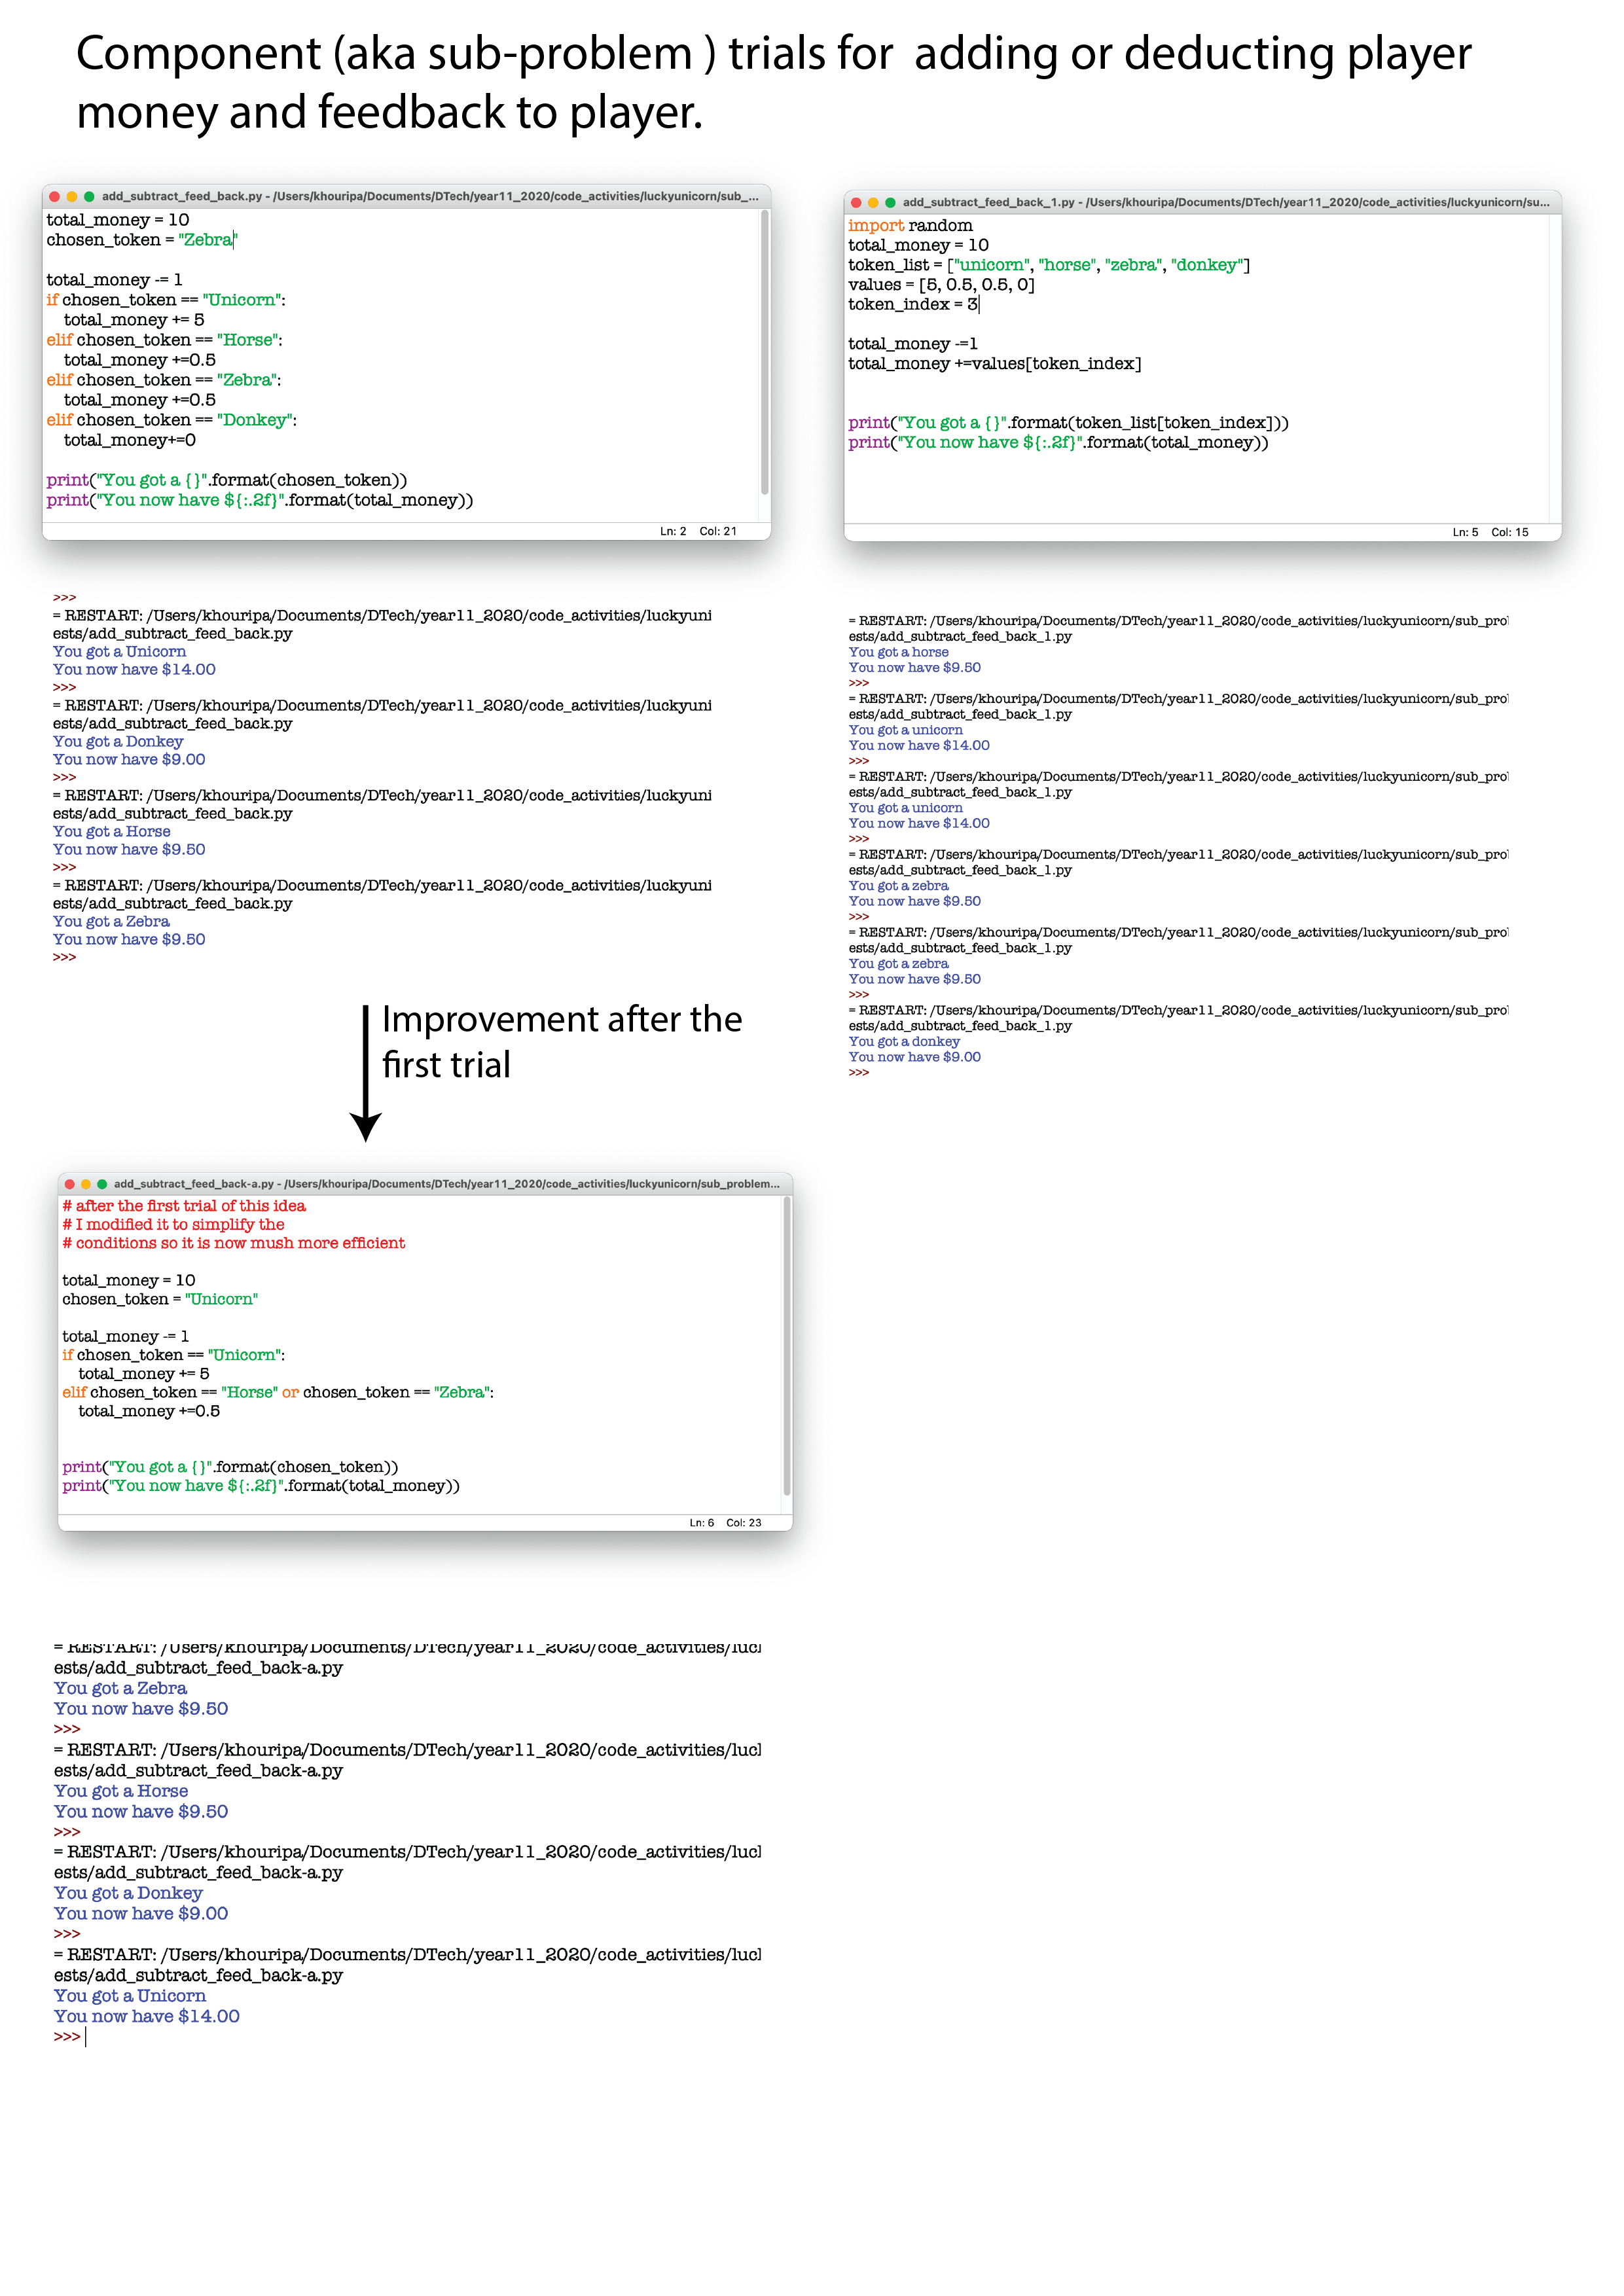
\includegraphics[width=17cm]{iterative_processes/sub_problem_trials_2.png}
	\caption*{Trialling different ways to solve the same sub-problem (the second)}
\end{figure}

\newpage

\begin{figure} [!h]
	\centering
	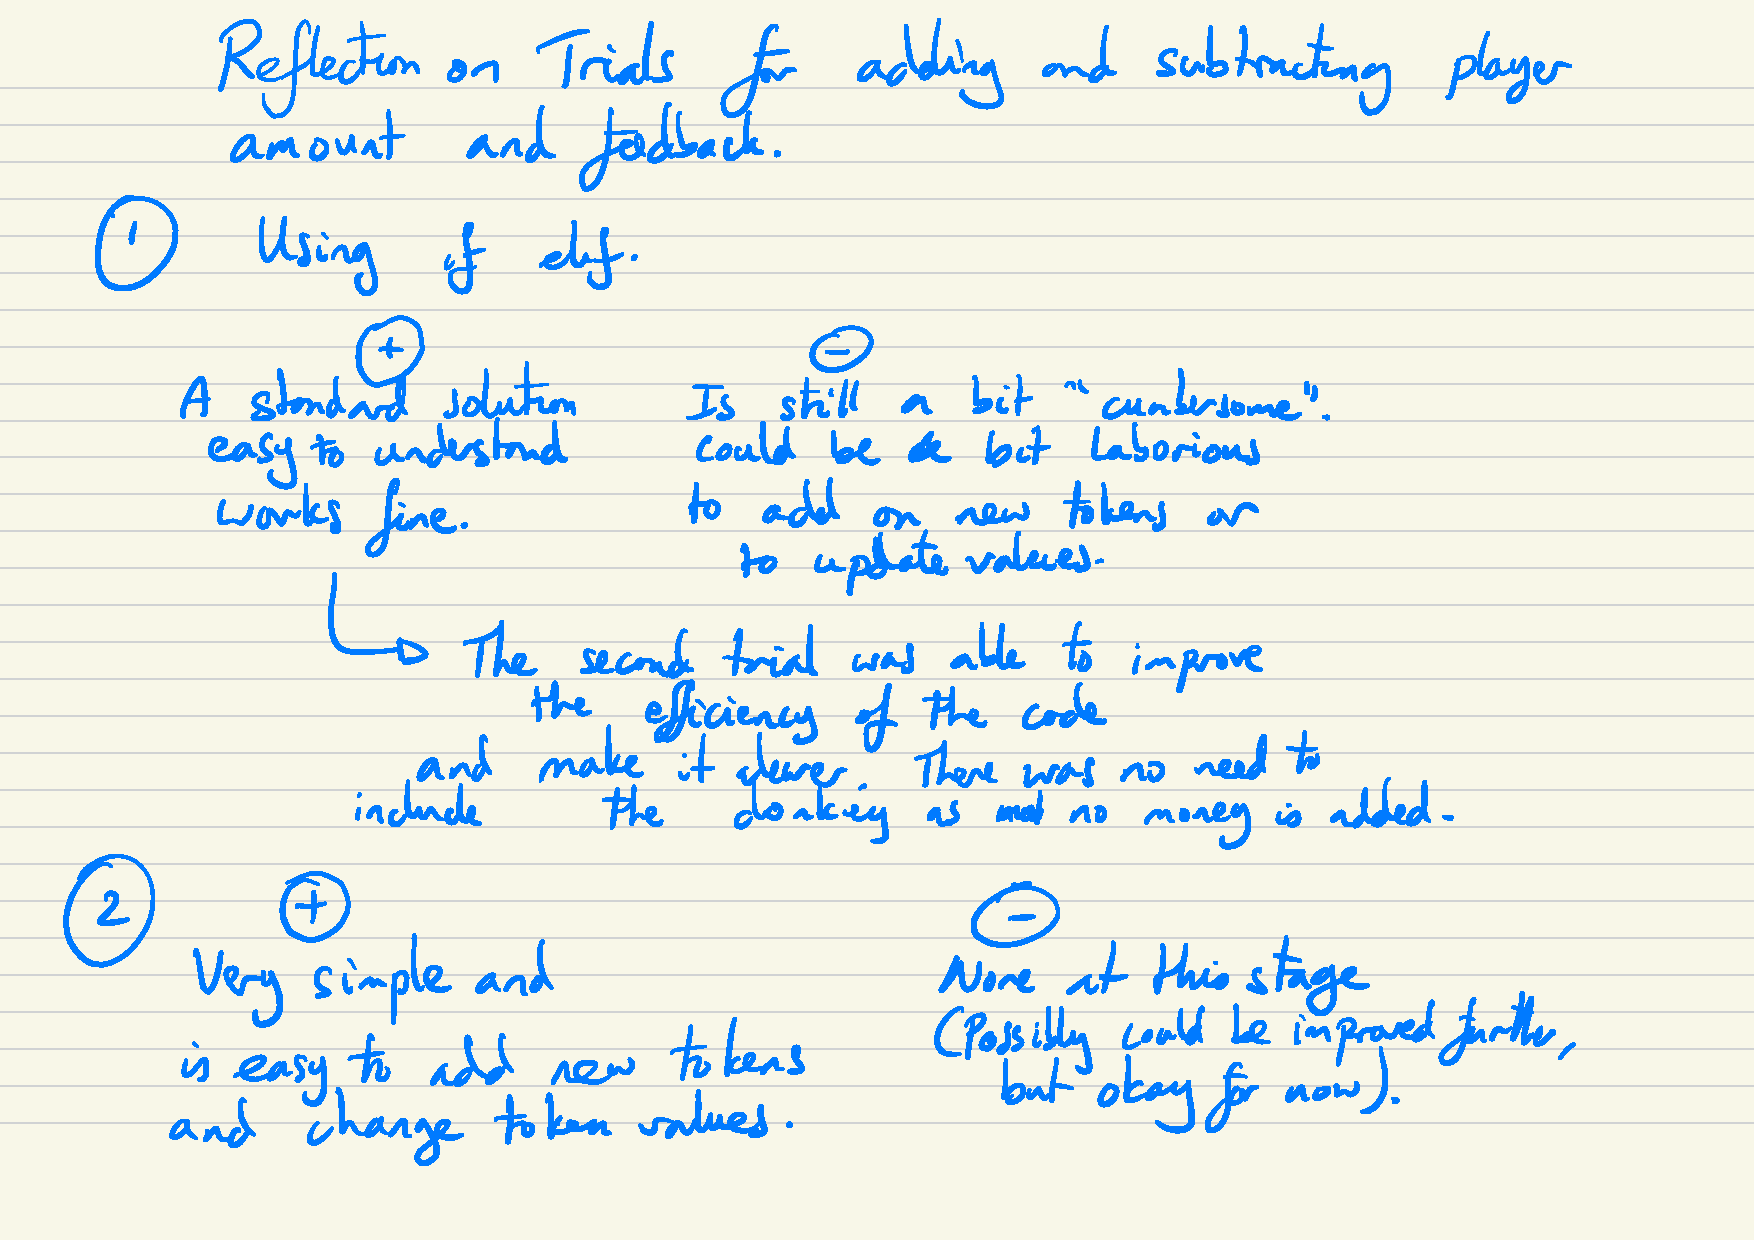
\includegraphics[width=15cm]{iterative_processes/Lucky_Unicorn_Sub_problems_3_a.pdf}
	\caption*{A reflection on the trials and a choice}
\end{figure}

\newpage
\lstinputlisting[language=Python, caption=Python example]{luckyunicorn/v1_lucky_unicorn.py}
\newpage


\section{Code Examples}
\subsection{Dinner Order}
\lstinputlisting[language=Python, caption = Dinner Order Program]{trinket/dinner_order_basic.py}
\subsection{Strawberry Picking}
\lstinputlisting[language=Python, caption=Python example]{strawberry_picking.py}
\subsection{Guess greater, less or equal}
%\lstset{style=mystyle_big}
\lstinputlisting[language=Python, caption=Python example]{trinket/random_choose_L_E_H.py}
%\lstset{style=mystyle}
\subsection{Higher Lower Game}
\lstinputlisting[language=Python, caption=Python example]{higher_lower.py}
\section{Testing}
\newpage
\section{Dictionaries}
\lstinputlisting[language=Python, caption=Python example]{dictionaries.py}
\lstinputlisting[language=Python, caption=Python example]{tommi.py}



\newpage
\section{Coffee}
\lstinputlisting[language=Python, caption=Python example]{class_randomletters_function.py}
\lstinputlisting[language=Python, caption=Python example]{buildingastring.py}
\lstinputlisting[language=Python, caption=Python example]{buildingastring_v2.py}
\lstinputlisting[language=Python, caption=Python example]{buildingastring_v3.py}
\lstinputlisting[language=Python, caption=Python example]{class_randomletters_testfor6.py}
\lstinputlisting[language=Python, caption=Python example]{class_randomletters_function_c_list.py}
\lstinputlisting[language=Python, caption=Python example]{class_randomletters_function_list.py}
\lstinputlisting[language=Python, caption=Python example]{class_randomletters_testfor7.py}
\lstinputlisting[language=Python, caption=Python example]{class_randomletters_testfor8.py}
\lstinputlisting[language=Python, caption=Python example]{class_randomletters.py}
\lstinputlisting[language=Python, caption=Python example]{class_randomletters_function_c.py}
\lstinputlisting[language=Python, caption=Python example]{class_randomletters_to_distribution.py}
\newpage
\section{Tests}
\lstinputlisting[language=Python, caption=Dice Roll]{v0_random.py}
\lstinputlisting[language=Python, caption=Python example]{checkinlist.py}
\lstinputlisting[language=Python, caption=Python example]{dictionary_test.py}
\lstinputlisting[language=Python, caption=Python example]{format_test.py}
\lstinputlisting[language=Python, caption=Python example]{hangman.py}
\section{Strings}
\lstinputlisting[language=Python, caption=Python example]{string_tests.py}
\lstinputlisting[language=Python, caption=Python example]{counting_string.py}
\section{Objects}
\lstinputlisting[language=Python, caption=Python example
]{classes_objects.py}

\lstinputlisting[language=Python, caption=Python example
]{classforglobals.py}

\lstinputlisting[language=Python, caption=Python example
]{class_quiz.py}

\newpage

\section{Extension}
\subsection{Basics}
Be able to work reasonably comfortably with loops lists and functions.\\
For example, be able to loop to create a number sequence 3, 9, 27,... and load this into a list\\
Ideally this is built as a function.
\subsection{Some foundations}
Create a function that takes a string for it argument and returns the string written backwards. (do not use built in methods such reverse)\\\\

Create a function that can generate prime numbers (assuming the program knows `nothing').\\\\
Algorithm:
\begin{itemize}
	\item start with a list prime\_list = [2,3]
	\item looping with numbers 4 - 100, 
	\begin{itemize}
		\item for each number start a second loop that loops through the prime list
		\item check if the number is divisible by each number in the prime\_list 
		\begin{itemize}
			\item 	if it is break out of the loop
			\item if this second loop completes, add the number to prime\_list
		\end{itemize}
	\end{itemize}
\item return the prime\_list
\end{itemize}

\subsection{Sorting}
Make a little function that given list and two index numbers will swap the items in the list.\\

Make a function that given an unordered list of numbers will sort the list from smallest to largest.\\

This is a foundational problem in Computer Science (yes Python has a sort function, but by making ourselves we learn a lot about algorithm design).\\
The algorithm that you want to use is \textbf{Selection Sort}.\\
Can look up.\\
Selection Sort is the simplest and worst sorting algorithm but is a great place to start.\\
We can look at others from there.



















\end{document}